\sloppy
\chapter{FUNKCIONALNI ZAHTJEVI}

\sloppy
\section*{Kontrola verzija}

U par rečenica opisati koji članovi tima su učestvovali u kreiranju ovog poglavlja.

\noindent Emir Duvnjak - FZ1, FZ7, FZ8

\noindent Tarik Hastor - FZ2

\noindent Zakir Šehić - FZ3 i FZ4

\noindent Edin Živojević - FZ5 i FZ6

\noindent Benjamin Baždar - FZ9 i FZ10


\sloppy  
\section{FZ1: Pregled i uređivanje predstava}  

\sloppy  
\subsection{Opis funkcionalnog zahtjeva}  
\begin{itemize}  
    \item \textbf{Poslovni proces}: Upravljanje repertoarom i prodajom karata
    \item \textbf{Vrste korisnika}: Administrator, Registrovani korisnik.  
    \item \textbf{Scenariji korištenja}:  
        \begin{enumerate}  
            \item \textbf{Promijenjen termin predstave-korisnik potvrđuje rezervaciju:} 

            
            Nakon pregleda detalja predstave (datum, vrijeme, glumci) administrator mijenja termin predstave i šalje obavještenje korisniku koji prihvata izmjenu odabranog termina i potvrđuje rezervaciju  
            
            \item \textbf{Promijenjen termin predstave-korisnik odustaje od rezervacije:} 

            
            Nakon pregleda detalja predstave administrator mijenja termin predstave i šalje obavještenje korisniku koji ne prihvata izmjenu odabranog termina i odustaje od rezervacije
  
            \item \textbf{Administrator odustaje od promjene termina:} 

            
            Nakon detaljnog pregleda detalja predstave administrator odustaje od promjene termina  
        \end{enumerate}
    \item \textbf{UML dijagram aktivnosti}: Prikazan na slici \ref{fig:fz1} 
\end{itemize}   
\begin{figure}[H]
    \centering
    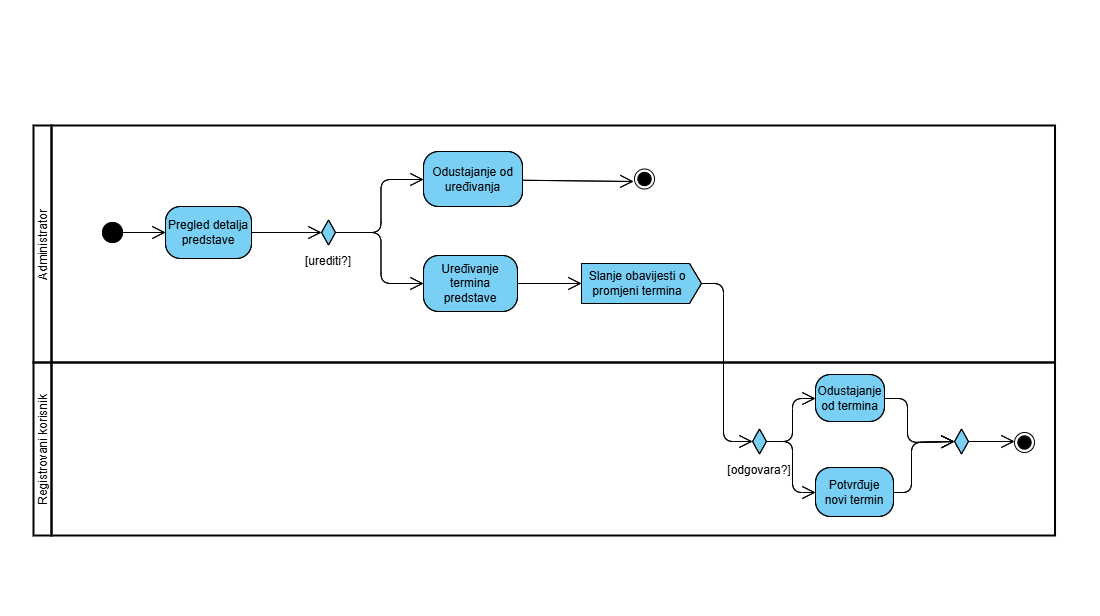
\includegraphics[width=1\textwidth]{Slike/Fz1.png}
    \caption{UML dijagram aktivnosti "Pregled i uređivanje predstava"}
    \label{fig:fz1}
\end{figure}

\sloppy  
\subsection{Dizajn korisničkih interfejsa}  
\begin{itemize}  
    \item \textbf{Prototip interfejsa}: Prikaz aktivnih predstava s opcijom uređivanja termina za administratore kao i pregleda izmijenjenih termina i aktivnih predstava za korisnike. Slike: \ref{fig:adminView} i \ref{fig:userView}
    \item \textbf{Opis scenarija}:  
        \begin{itemize}  
            \item Administrator pomiče predstavu u kalendaru i šalje obavijest korisnicima.  
            \item Korisnik pregleda ažurirani raspored i potvrđuje novi termin.  
        \end{itemize}  
\end{itemize}   

\begin{figure}[H]
    \centering
    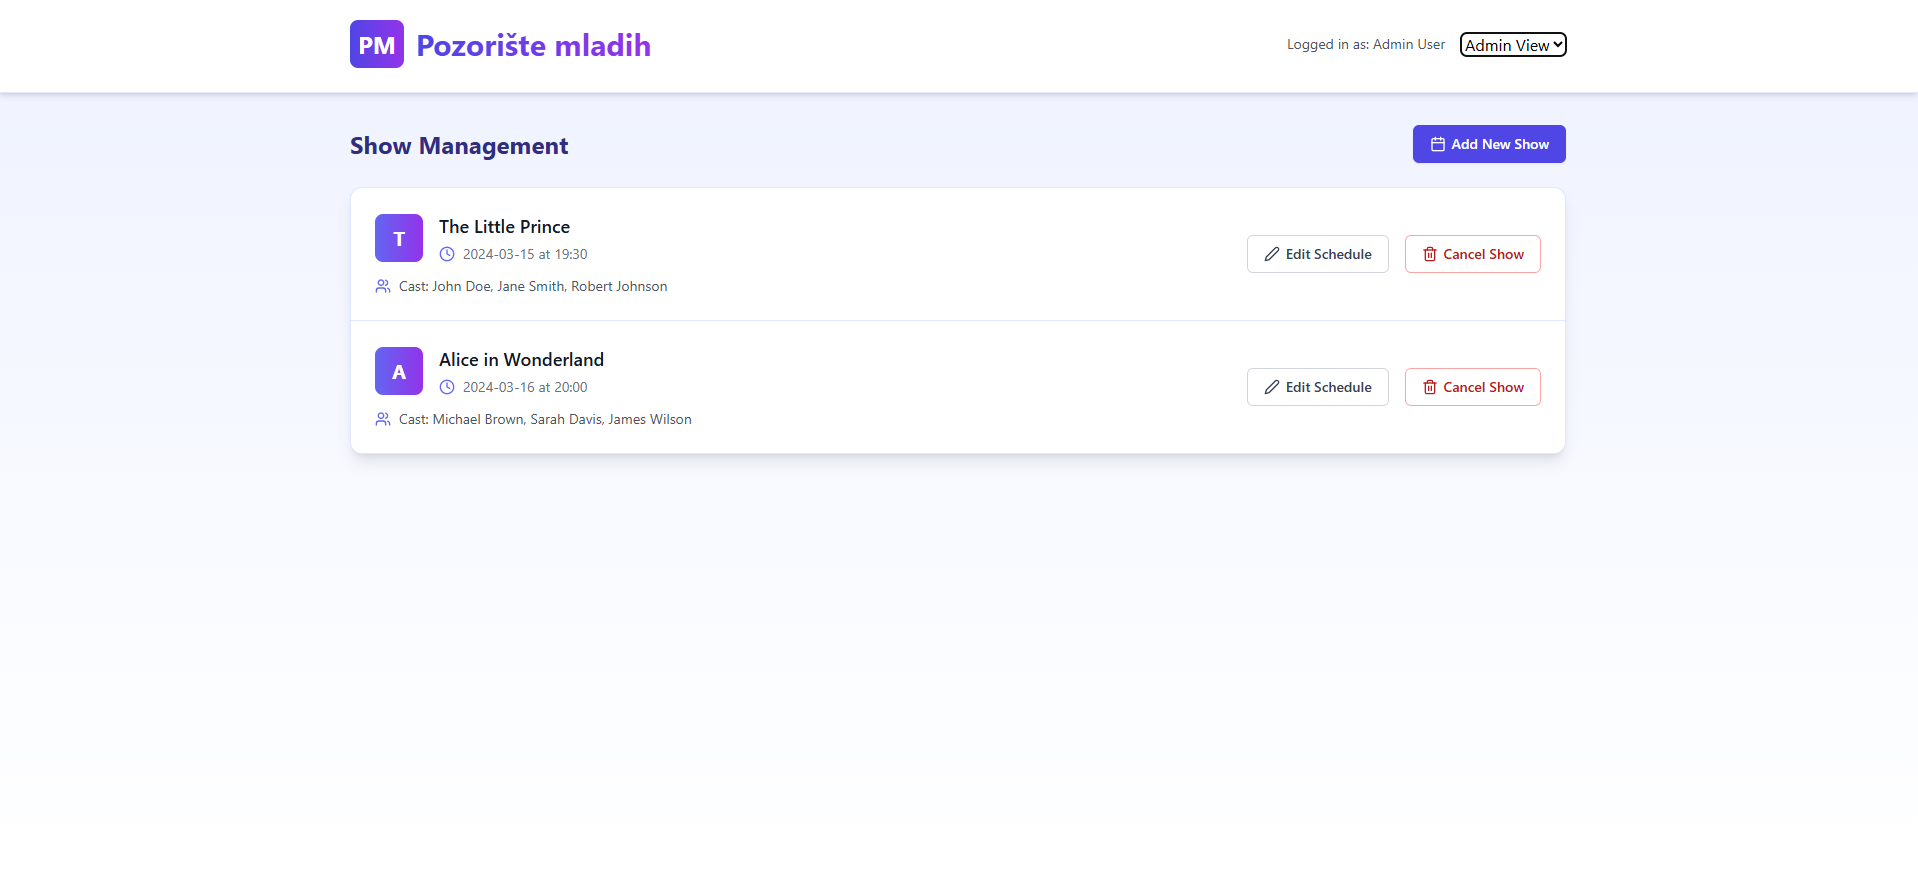
\includegraphics[width=1\textwidth]{Slike/adminView.PNG}
    \caption{Prototip interfejsa administratora za "Pregled i uređivanje predstava"}
    \label{fig:adminView}
\end{figure} 

\begin{figure}[H]
    \centering
    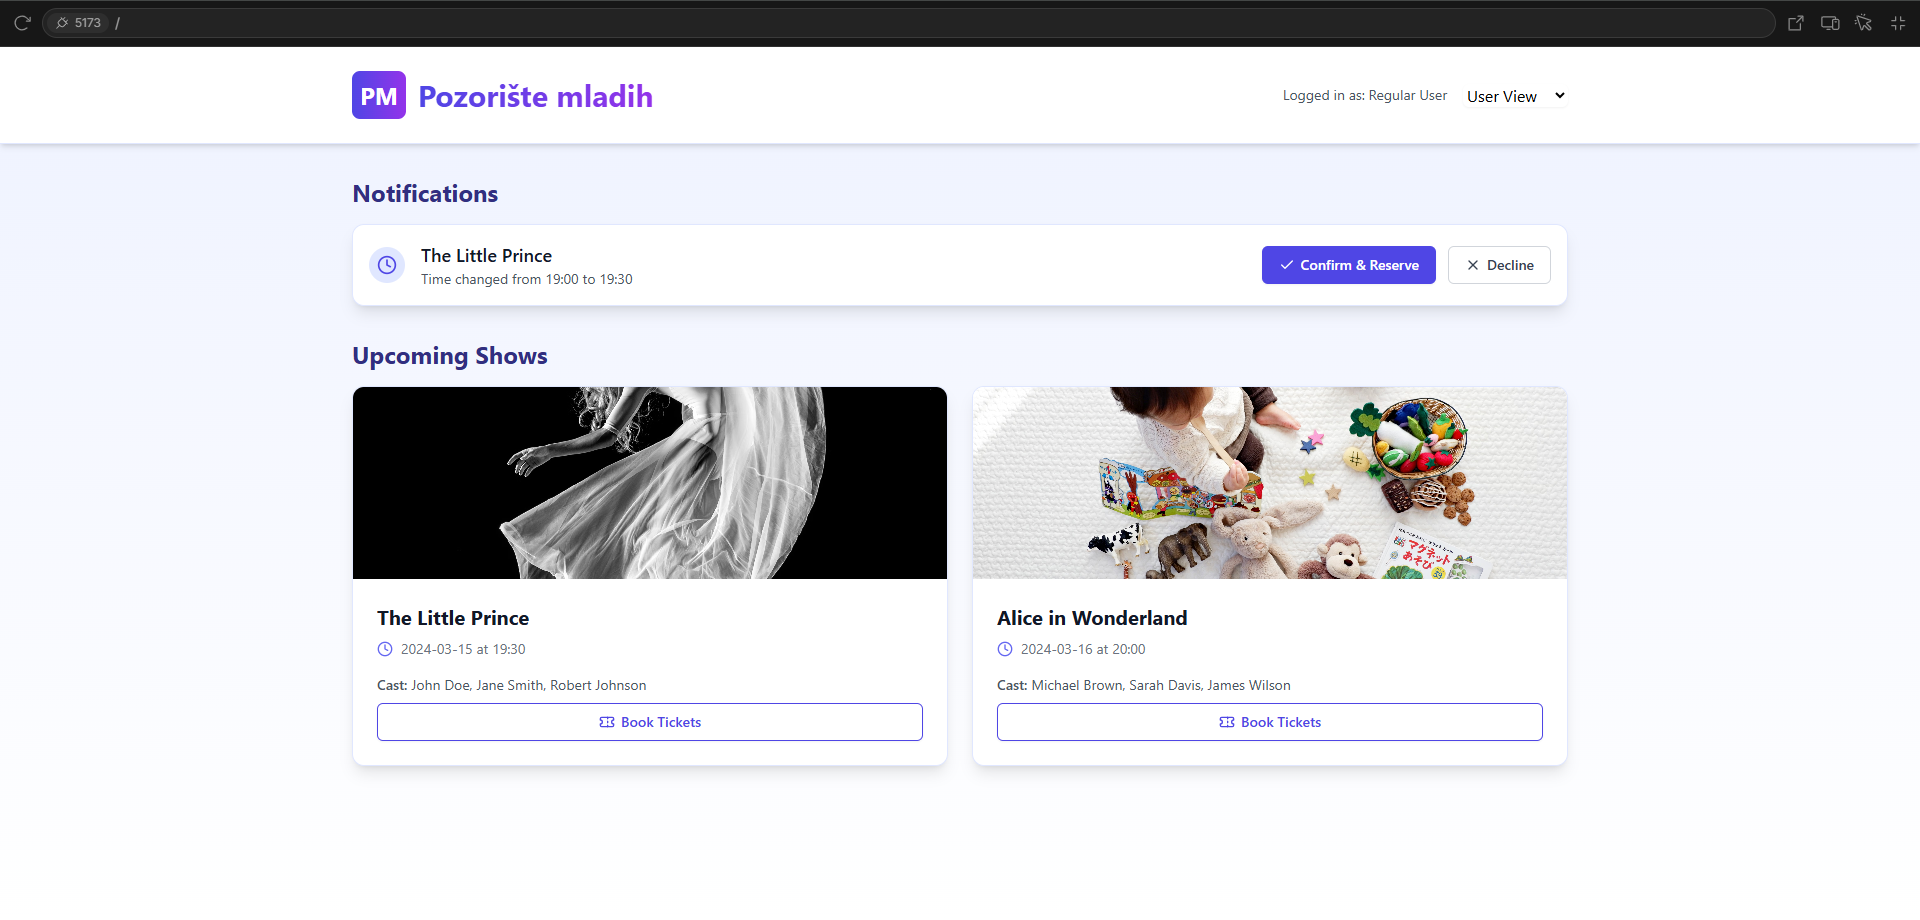
\includegraphics[width=1\textwidth]{Slike/userView.PNG}
    \caption{Prototip interfejsa korisnika za pregled izmijenjenih termina i aktivnih predstava}
    \label{fig:userView}
\end{figure}
\subsection{Bolt \textit{promptovi}}
\begin{enumerate}  
            \item \textbf{Prvi \textit{prompt}:}
            
            \textit{"Design a modern and user-friendly webpage for managing show schedules. The design should include distinct sections or interfaces for administrators and registered users, reflecting the following functionalities:}
        
            \textit{Administrator Interface:}
            
            \textit{Show Details View: A section where administrators can view a list of shows with their details, including date, time, and actors.
            Edit Functionality: An option (like an 'Edit' button) for each show that allows administrators to modify its schedule (specifically the time).
            Notification System: After editing a show's time, the system should prompt the administrator to send a notification about this change to all registered users.
            Cancel Edit Option: During the editing process, administrators should have an option to cancel their changes.}
            \textit{Registered User Interface:
            Notification Display: A section where registered users can view notifications about changes to show times.
            Updated Schedule View: Users should be able to see the updated schedule of shows.
            Confirmation/Rejection: For each notification about a time change, users should have clear options to either 'Confirm' the new time or 'Decline' it.
            The overall design should be clean, modern, and easy to navigate for both administrators and registered users. Consider using a visually appealing layout and intuitive controls for each action."}


            
            \item \textbf{Drugi \textit{prompt}:}
            
            \textit{"Building upon the previous request for a webpage design to manage show schedules, please make the following enhancements:}

            \textit{Modern Design  Youth Theater Theme: Update the overall design to be more modern and visually appealing, with a style that is suitable for a youth theater. Consider using a vibrant color palette and playful design elements to create an energetic and engaging user experience.}
            
            \textit{Notification Specificity: When displaying notifications to registered users about show time changes, ensure that each notification clearly states which show the time change is for.
            Reservation Integration: For registered users, when they click the 'Confirm' button on a notification regarding a show time change, instead of just confirming, the action should redirect them to a reservation or booking screen specifically for that show and the new time. This will allow them to immediately proceed with booking tickets for the updated schedule."}


  
            \item \textbf{Treći \textit{prompt}:}
            
            \textit{Please fix the image on the Alice in Wonderland page. Additionally, in the admin section, add functionality to modify the date as well as the time of an event. There should also be an option to cancel the entire show. Ensure all these changes are reflected for the user. Furthermore, when viewing as a regular user, the display should say 'Logged in as User' instead of 'admin'.}
        \end{enumerate}

\sloppy  
\section{FZ2: \textit{Online} prodaja i rezervacija karata s višestrukim načinima plaćanja}  



\sloppy  
\subsection{Opis funkcionalnog zahtjeva}  
\begin{itemize}  
    \item \textbf{Poslovni proces}: Upravljanje repertoarom i prodajom karata 
    \item \textbf{Vrste korisnika}: Gost, Registrovani korisnik 
    \item \textbf{Scenariji korištenja}:  
        \begin{enumerate}  
            \item Neregistrovani korisnik pregleda predstave, dodaje željenu u korpu i rezerviše unosom podataka za rezervaciju. Sistem obavještava o uspješnosti rezervacije.  
            \item Registrovani korisnik pregleda dostupne predstave, dodaje željenu u korpu i odabira rezervaciju sa plaćanjem te bira načina plaćanja (kreditna kartica, \textit{Google Pay, PayPal}). Sistem obavještava o uspješnosti rezervacije.  
            \item Registrovani korisnik pregleda dostupne predstave, dodaje željenu u korpu i odabira rezervaciju bez plaćanja gdje se njegovi podaci automatski unose. Sistem obavještava o uspješnosti rezervacije.  
        \end{enumerate}  
    \item \textbf{UML dijagram aktivnosti}: Prikazan na slici \ref{fig:fz2}.  
\end{itemize}  
\begin{figure}[H]
    \centering
    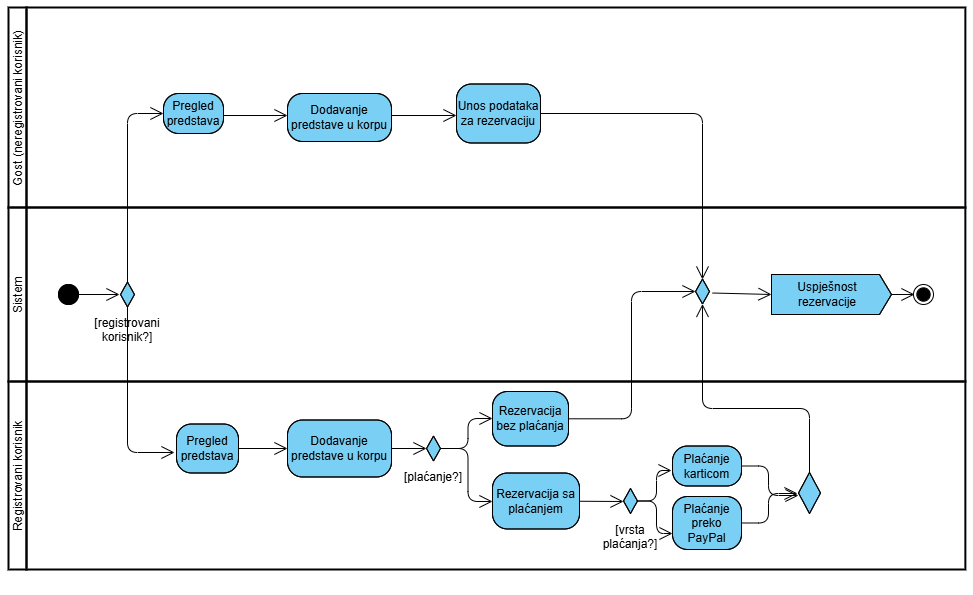
\includegraphics[width=0.8\textwidth]{Slike/Fz2.png}
    \caption{UML dijagram aktivnosti "\textit{Online} prodaja i rezervacija karata"}
    \label{fig:fz2}
\end{figure}
\sloppy  
    \textbf{Opis scenarija}:  
        \begin{itemize}  
            \item Korisnik bira predstavu, odabire sjedište klikom na mapu, te odabire način plaćanja.  
            \item Gost mora unijeti osnovne podatke (ime, e-mail) za rezervaciju.  
        \end{itemize}  
\subsection{Dizajn korisničkih interfejsa}  
\begin{itemize}  
    \item \textbf{Prototip interfejsa}: Interfejsi koji odgovara prethodno navedenim zahtjevima prikazani su na slikama \ref{fig:userfront}, \ref{fig:userselect}, \ref{fig:userview}, \ref{fig:usercheckout}, \ref{fig:userfrontlist},  \ref{fig:guesthome}, \ref{fig:questcheck}
\begin{figure}[H]
    \centering
    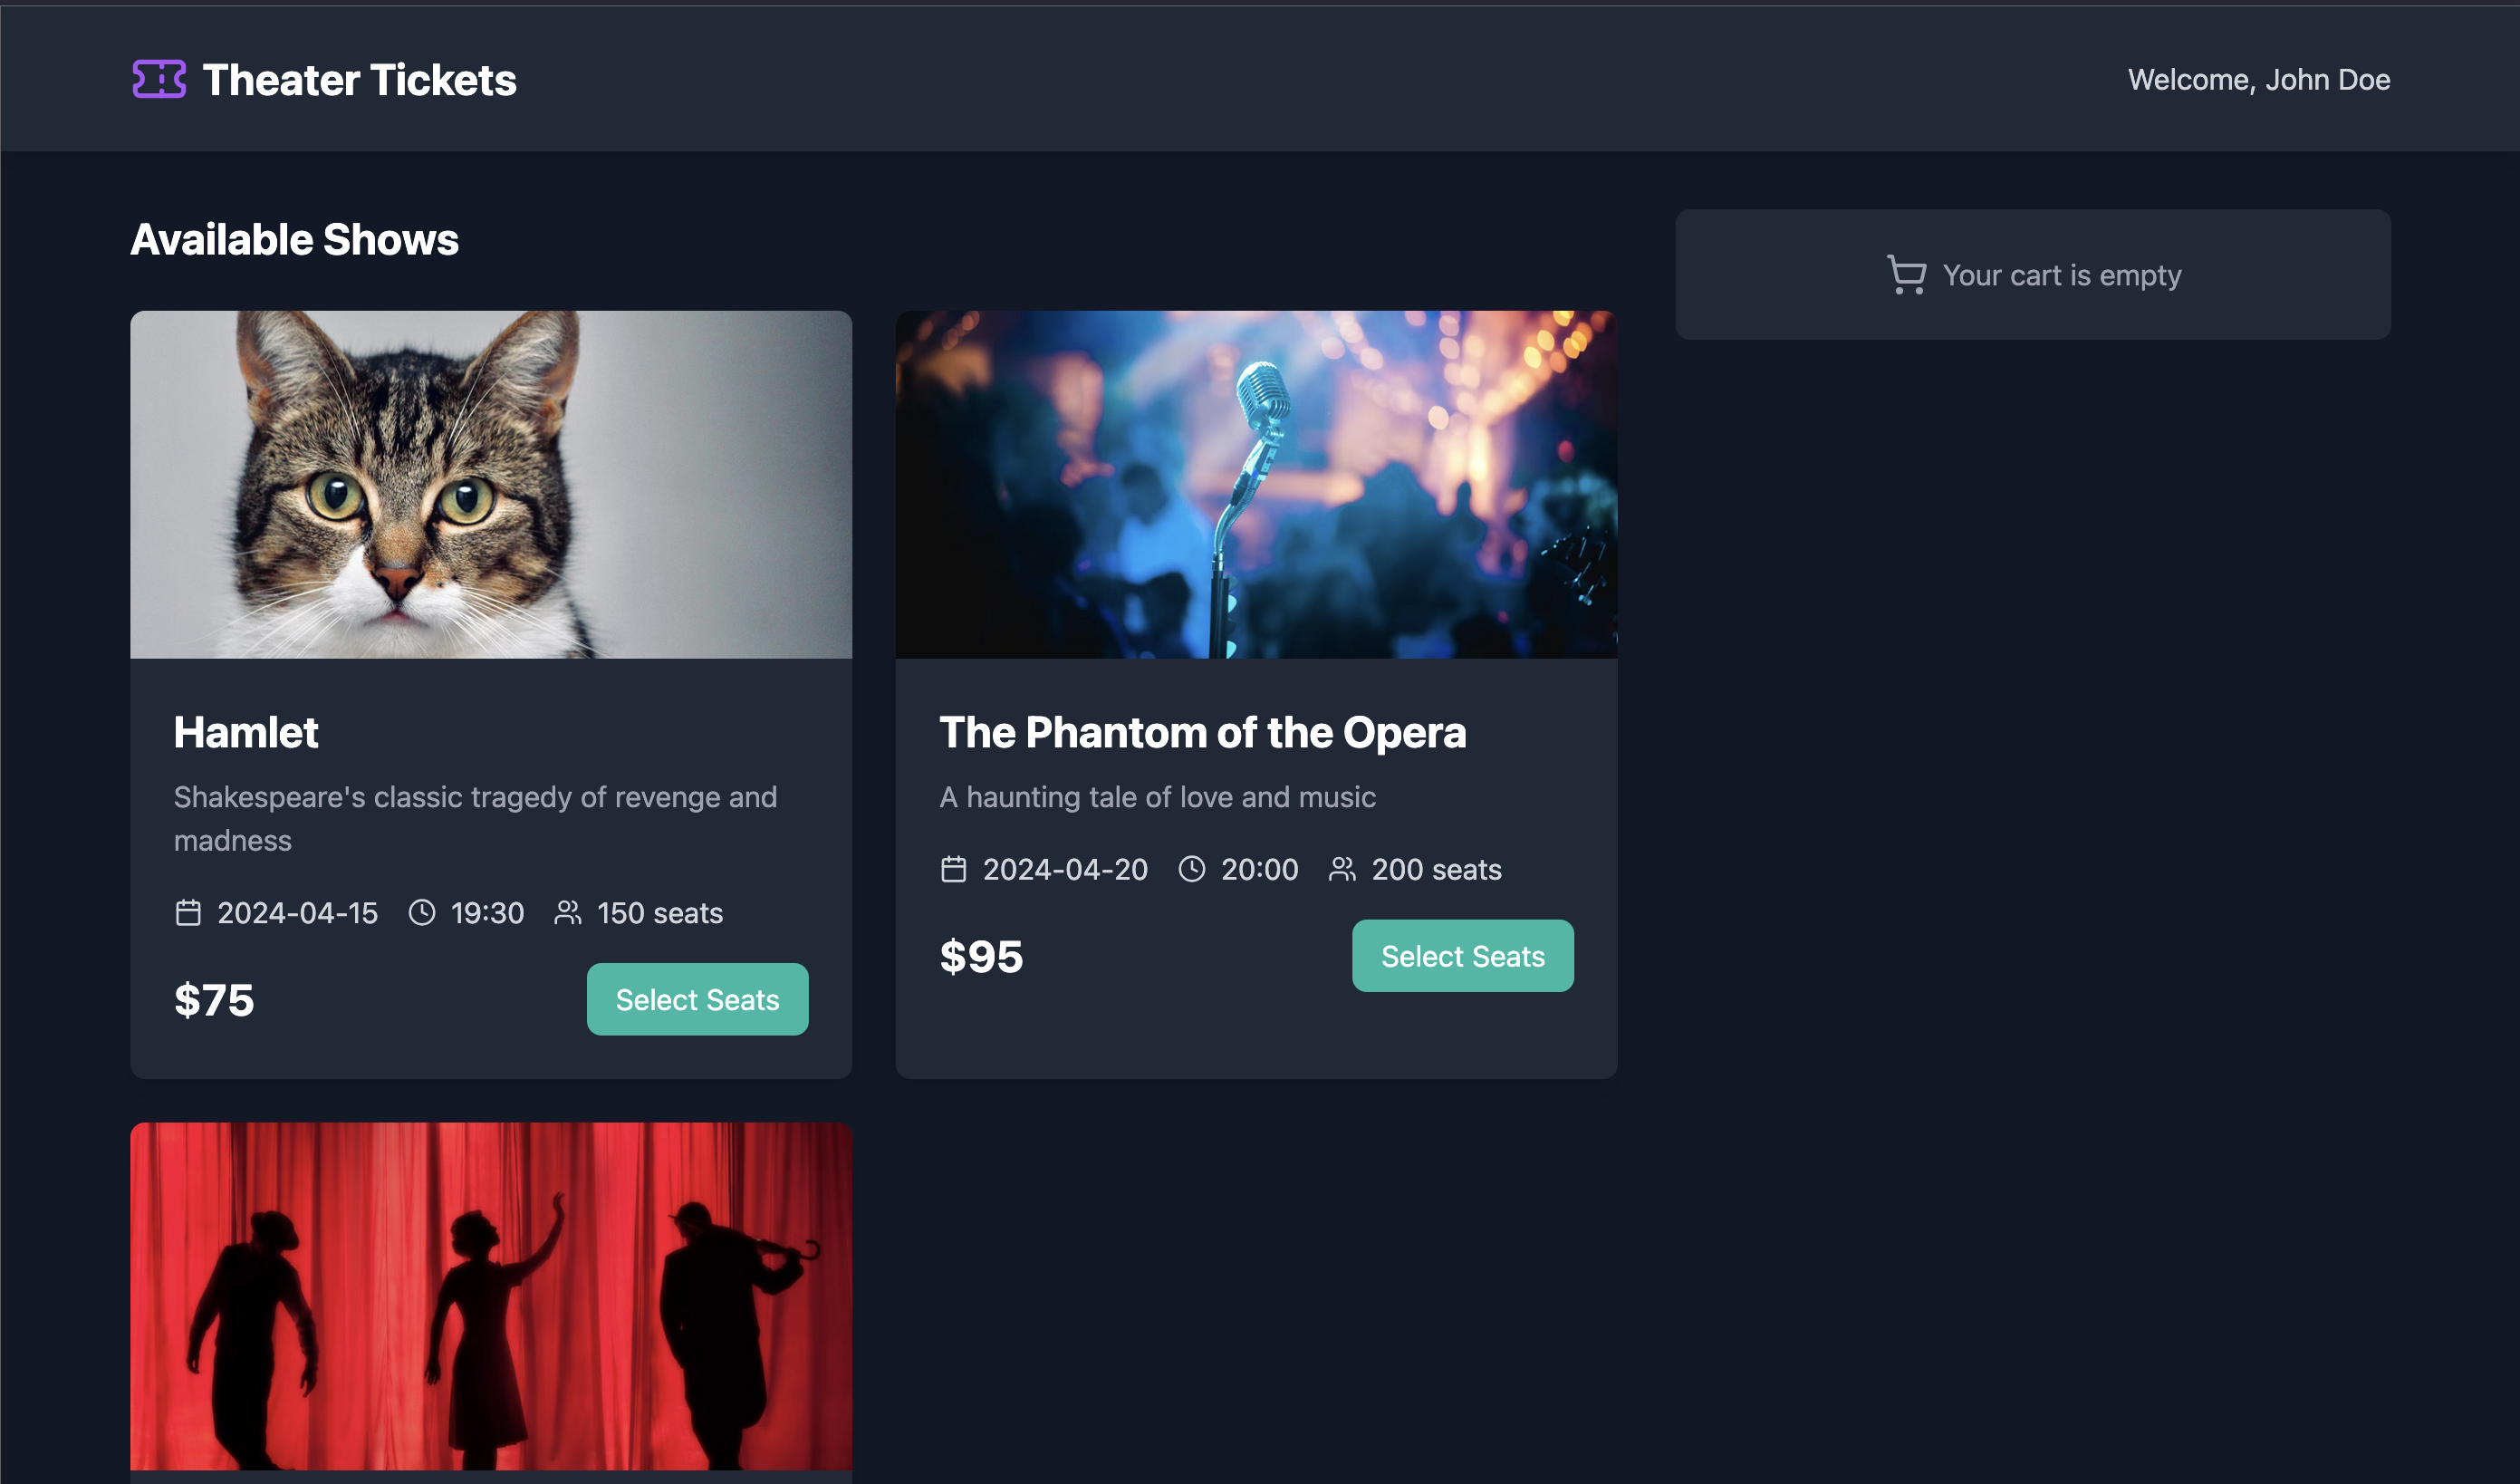
\includegraphics[width=0.9\textwidth]{Slike/FZ2ui/userfront.png}
    \caption{Prototip interfejsa korisnika za pregled predstava}
    \label{fig:userfront}
\end{figure} 
\begin{figure}[H]
    \centering
    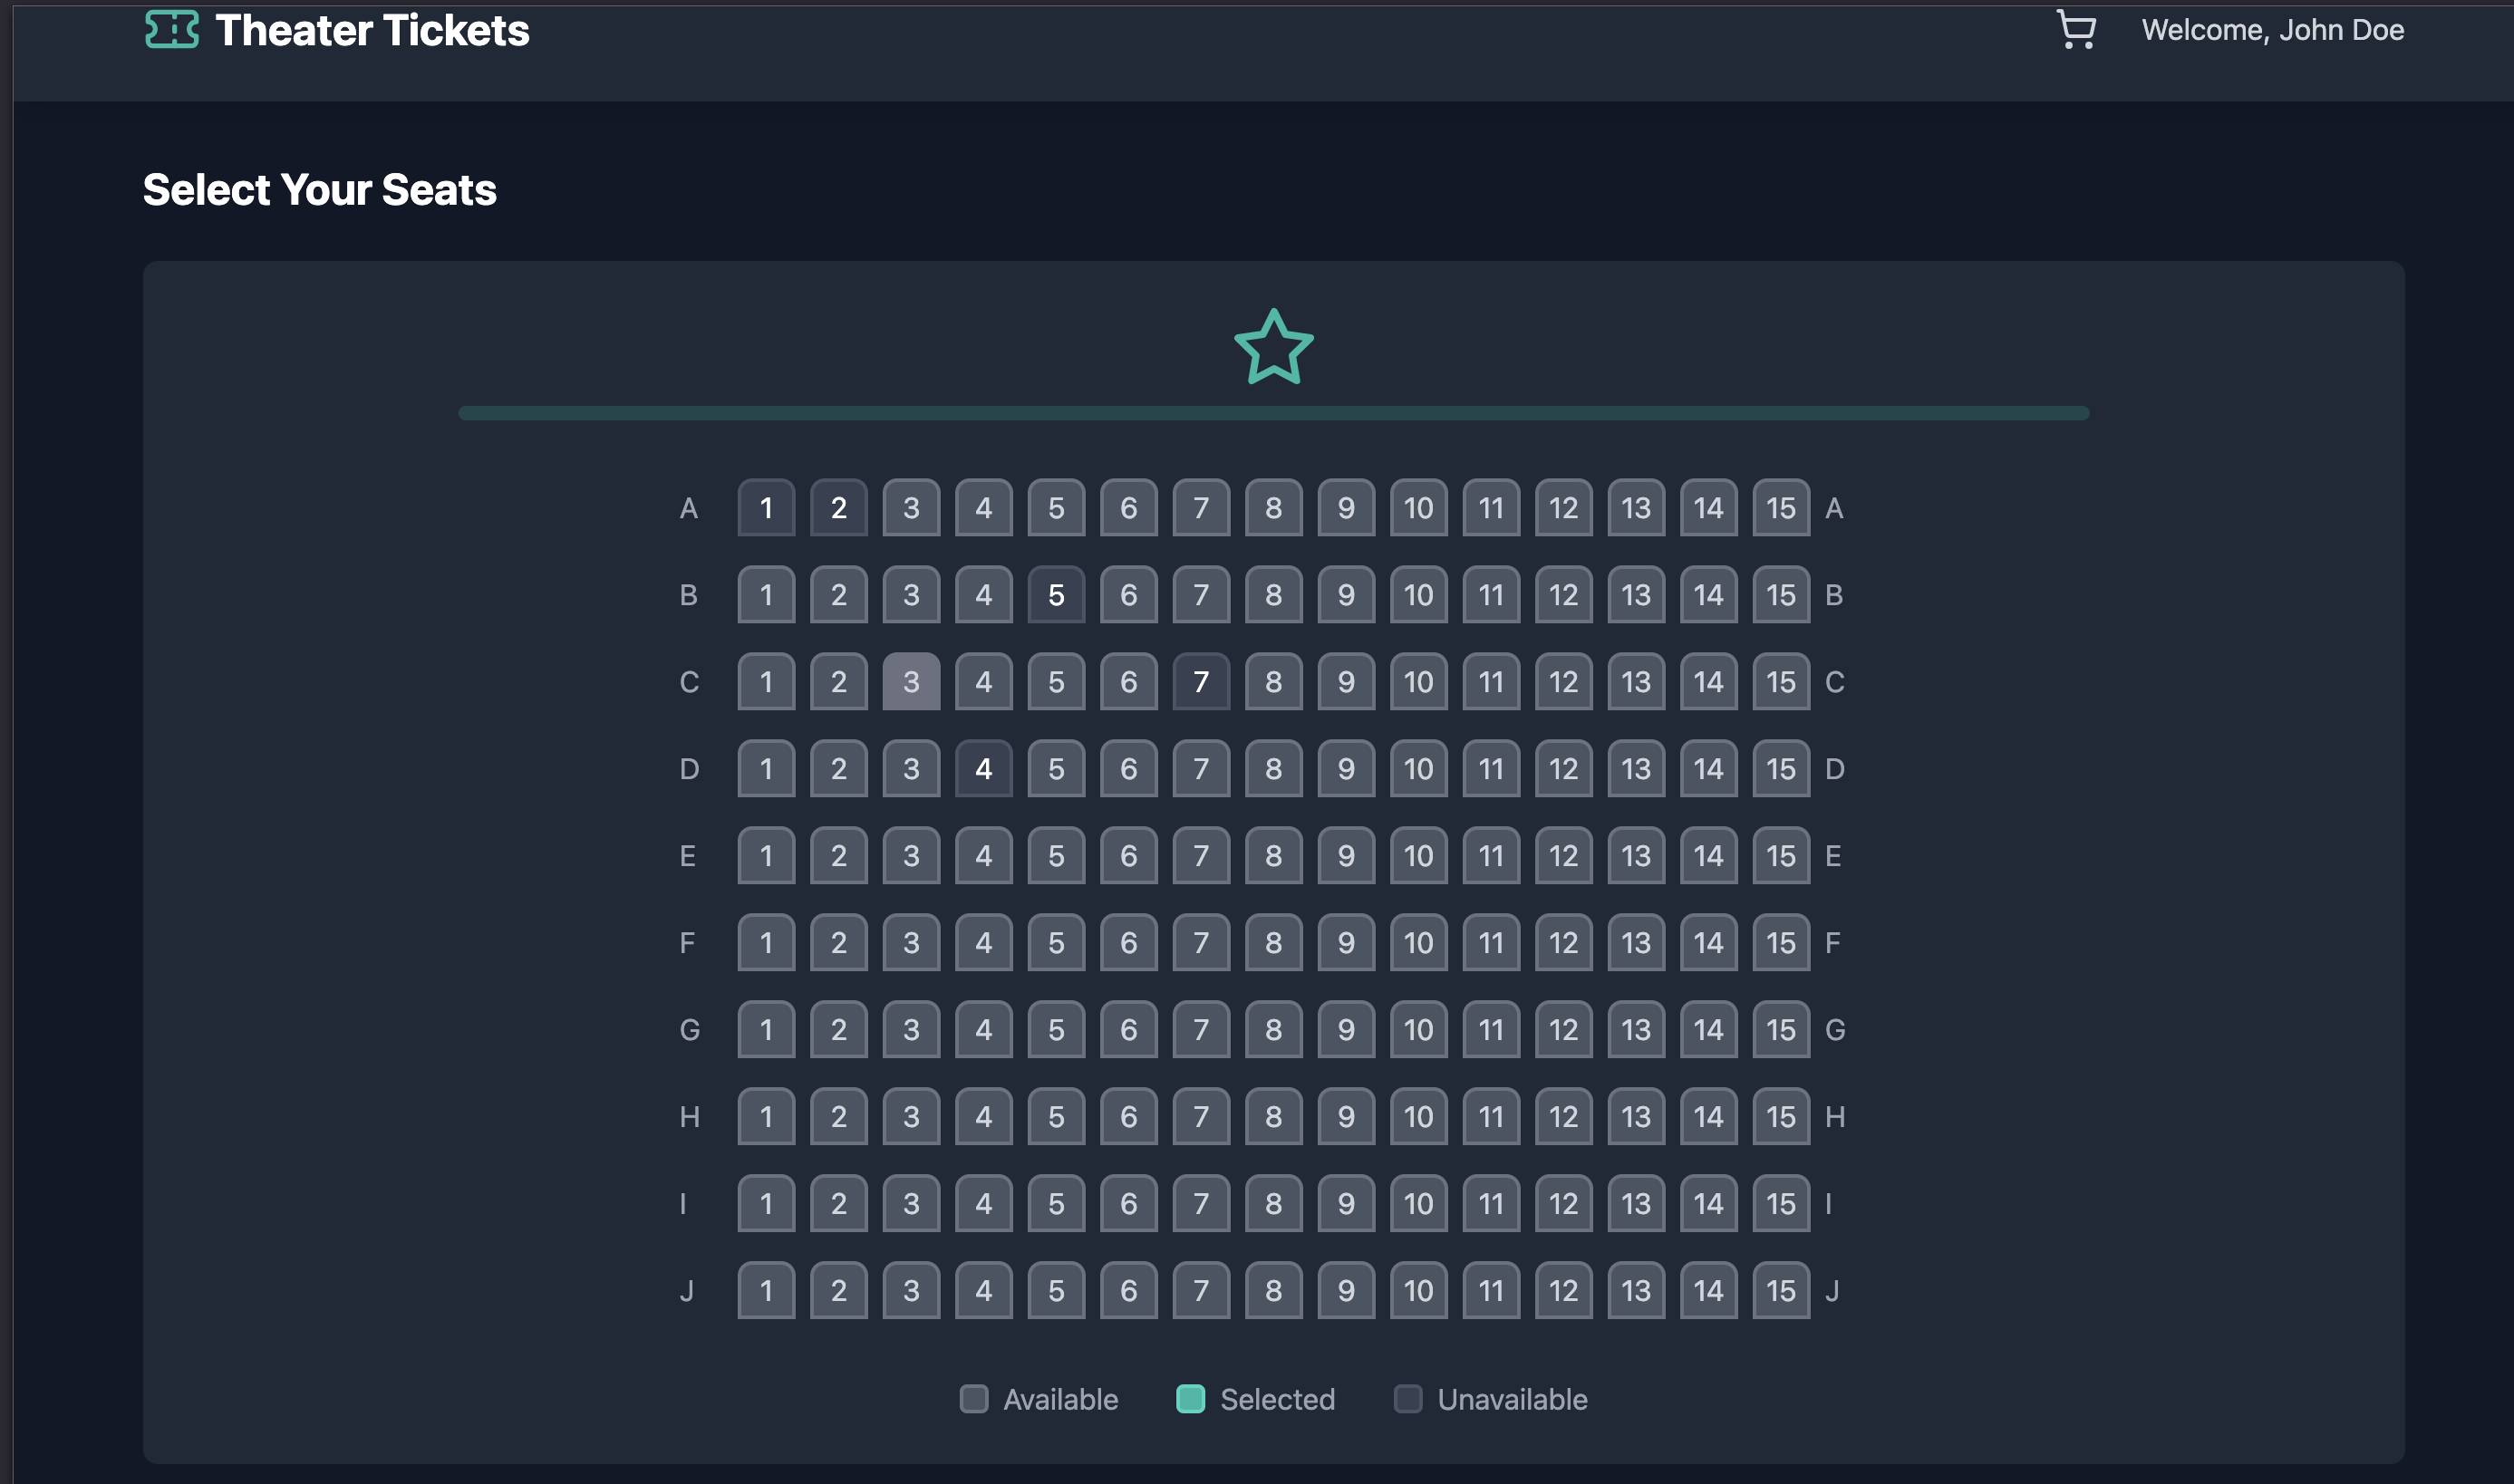
\includegraphics[width=0.9\textwidth]{Slike/FZ2ui/userselect.png}
    \caption{Prototip interfejsa korisnika za pregled i odabir slobodnih mjesta}
    \label{fig:userselect}
\end{figure}
\begin{figure}[H]
    \centering
    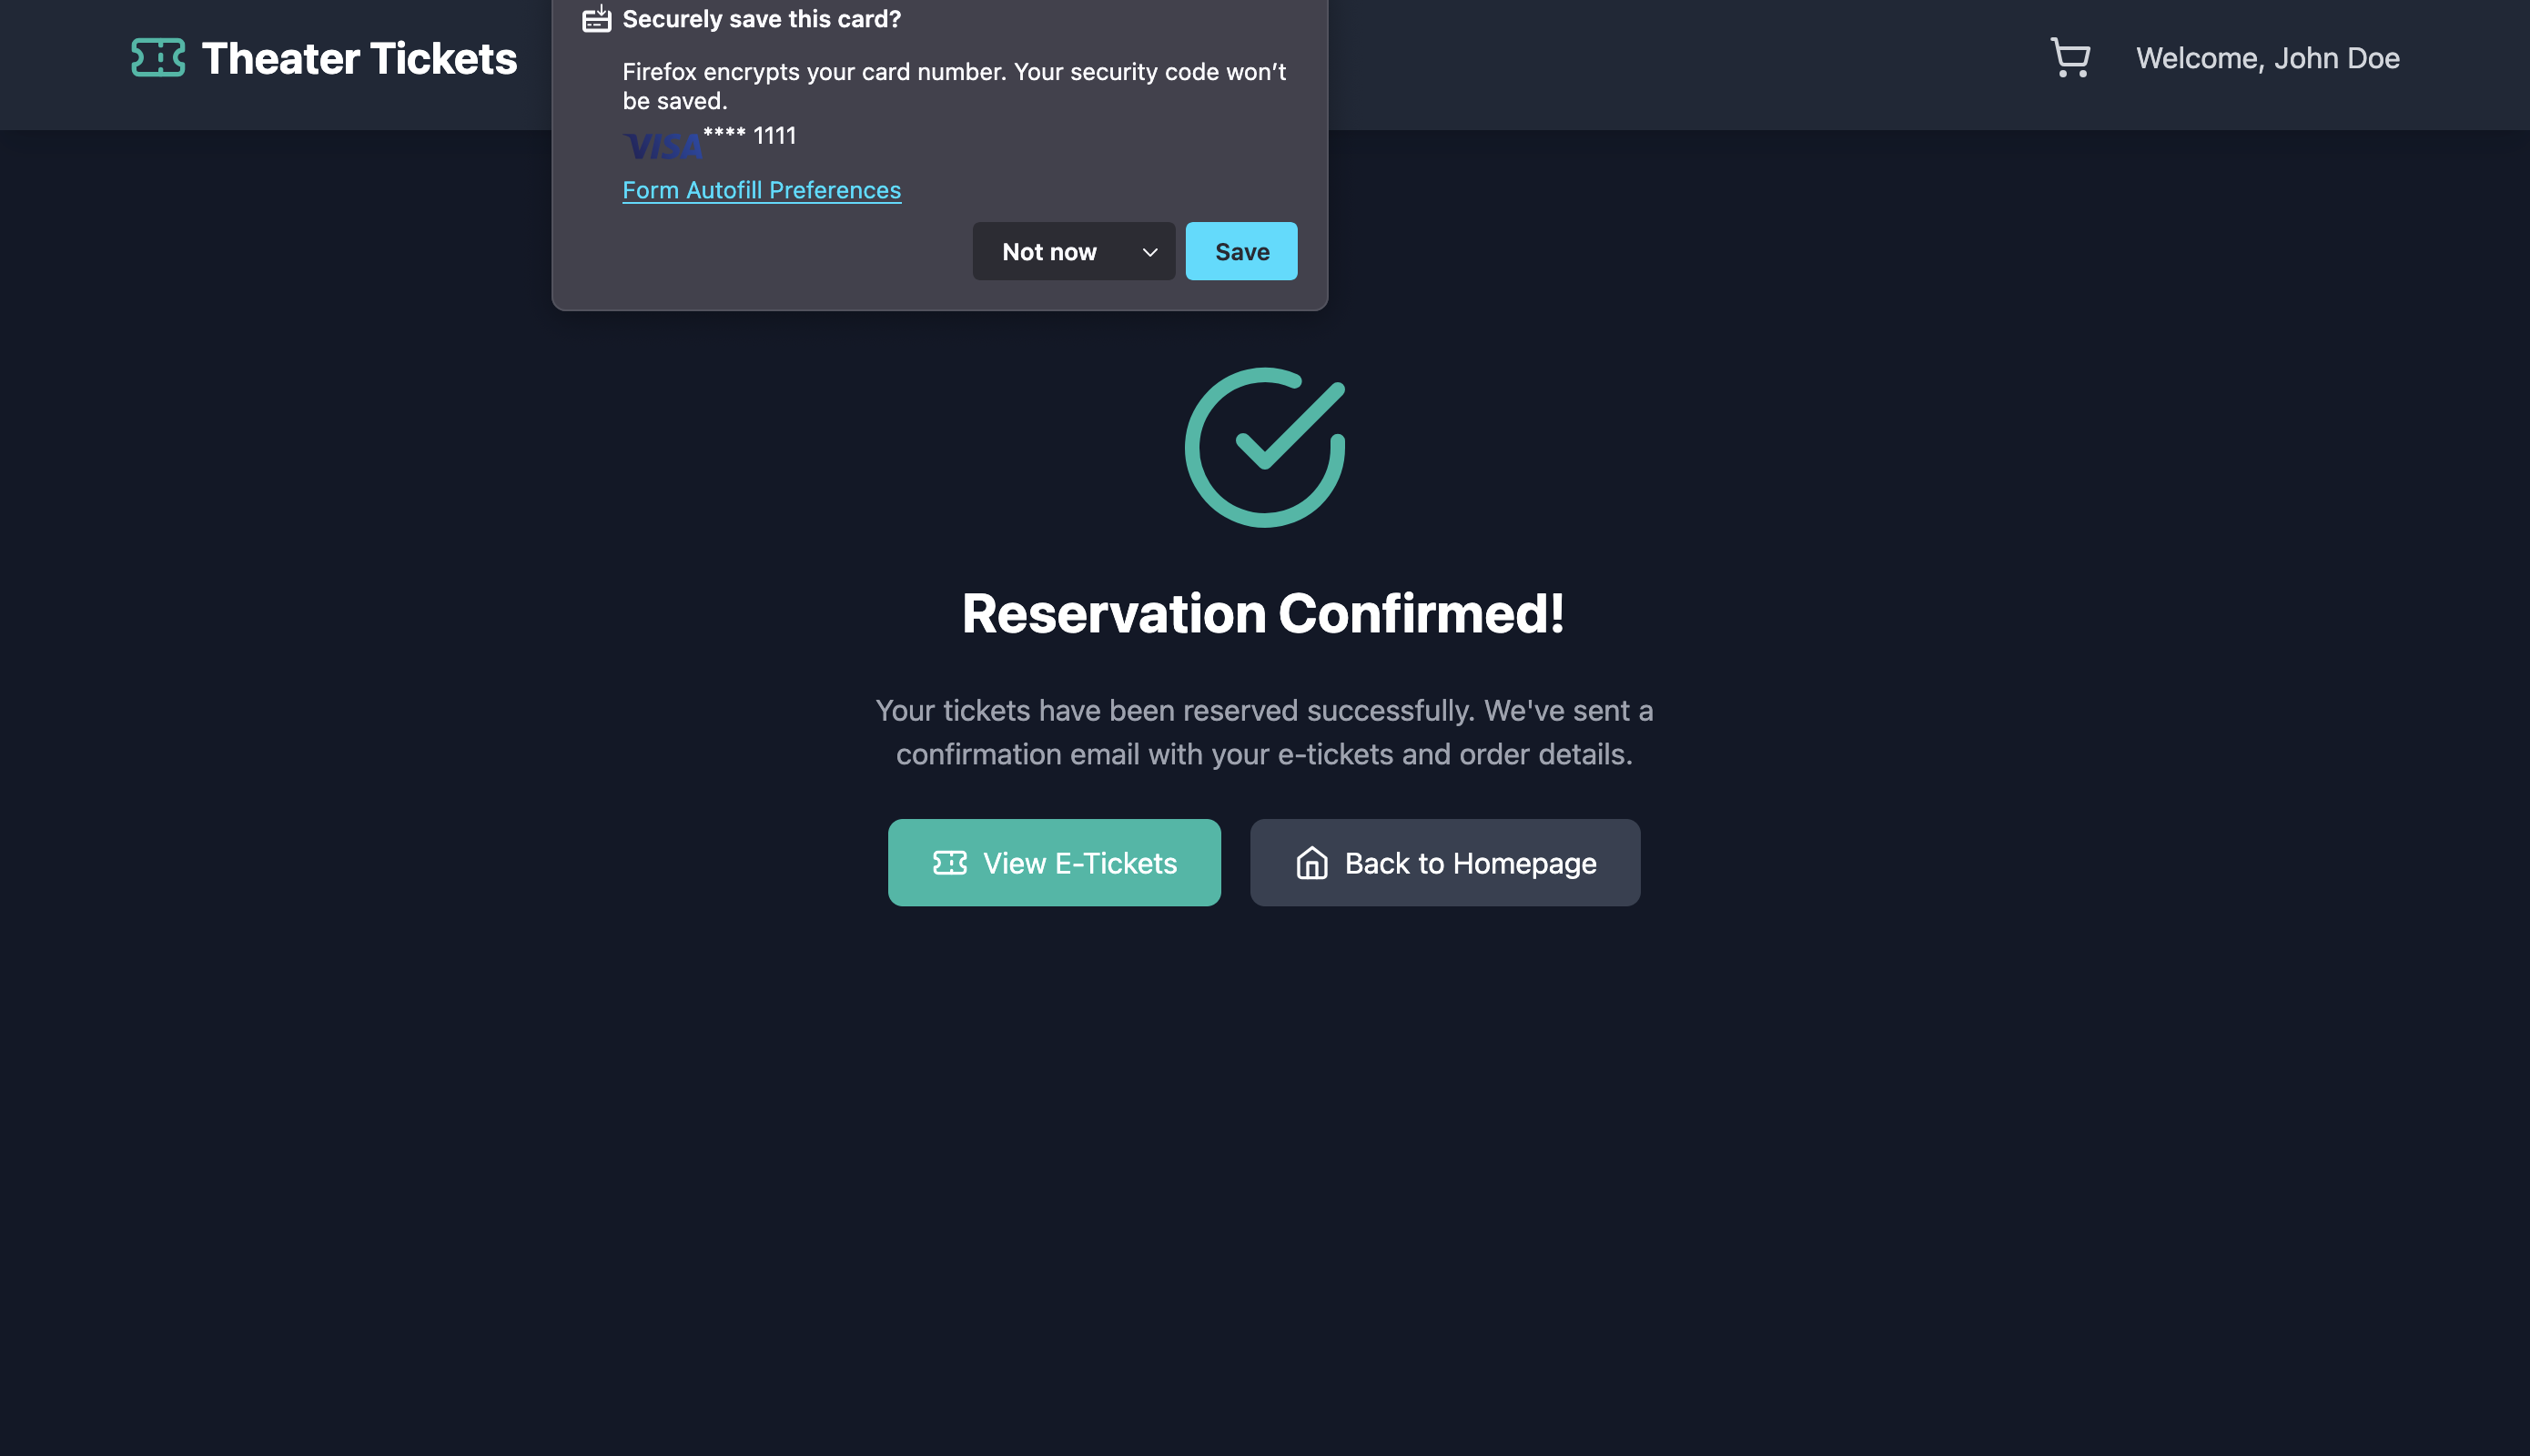
\includegraphics[width=0.9\textwidth]{Slike/FZ2ui/usercomplete.png}
    \caption{Prototip interfejsa za obavijest o uspješnoj registraciji predstave}
    \label{fig:userview}
\end{figure}
\begin{figure}[H]
    \centering
    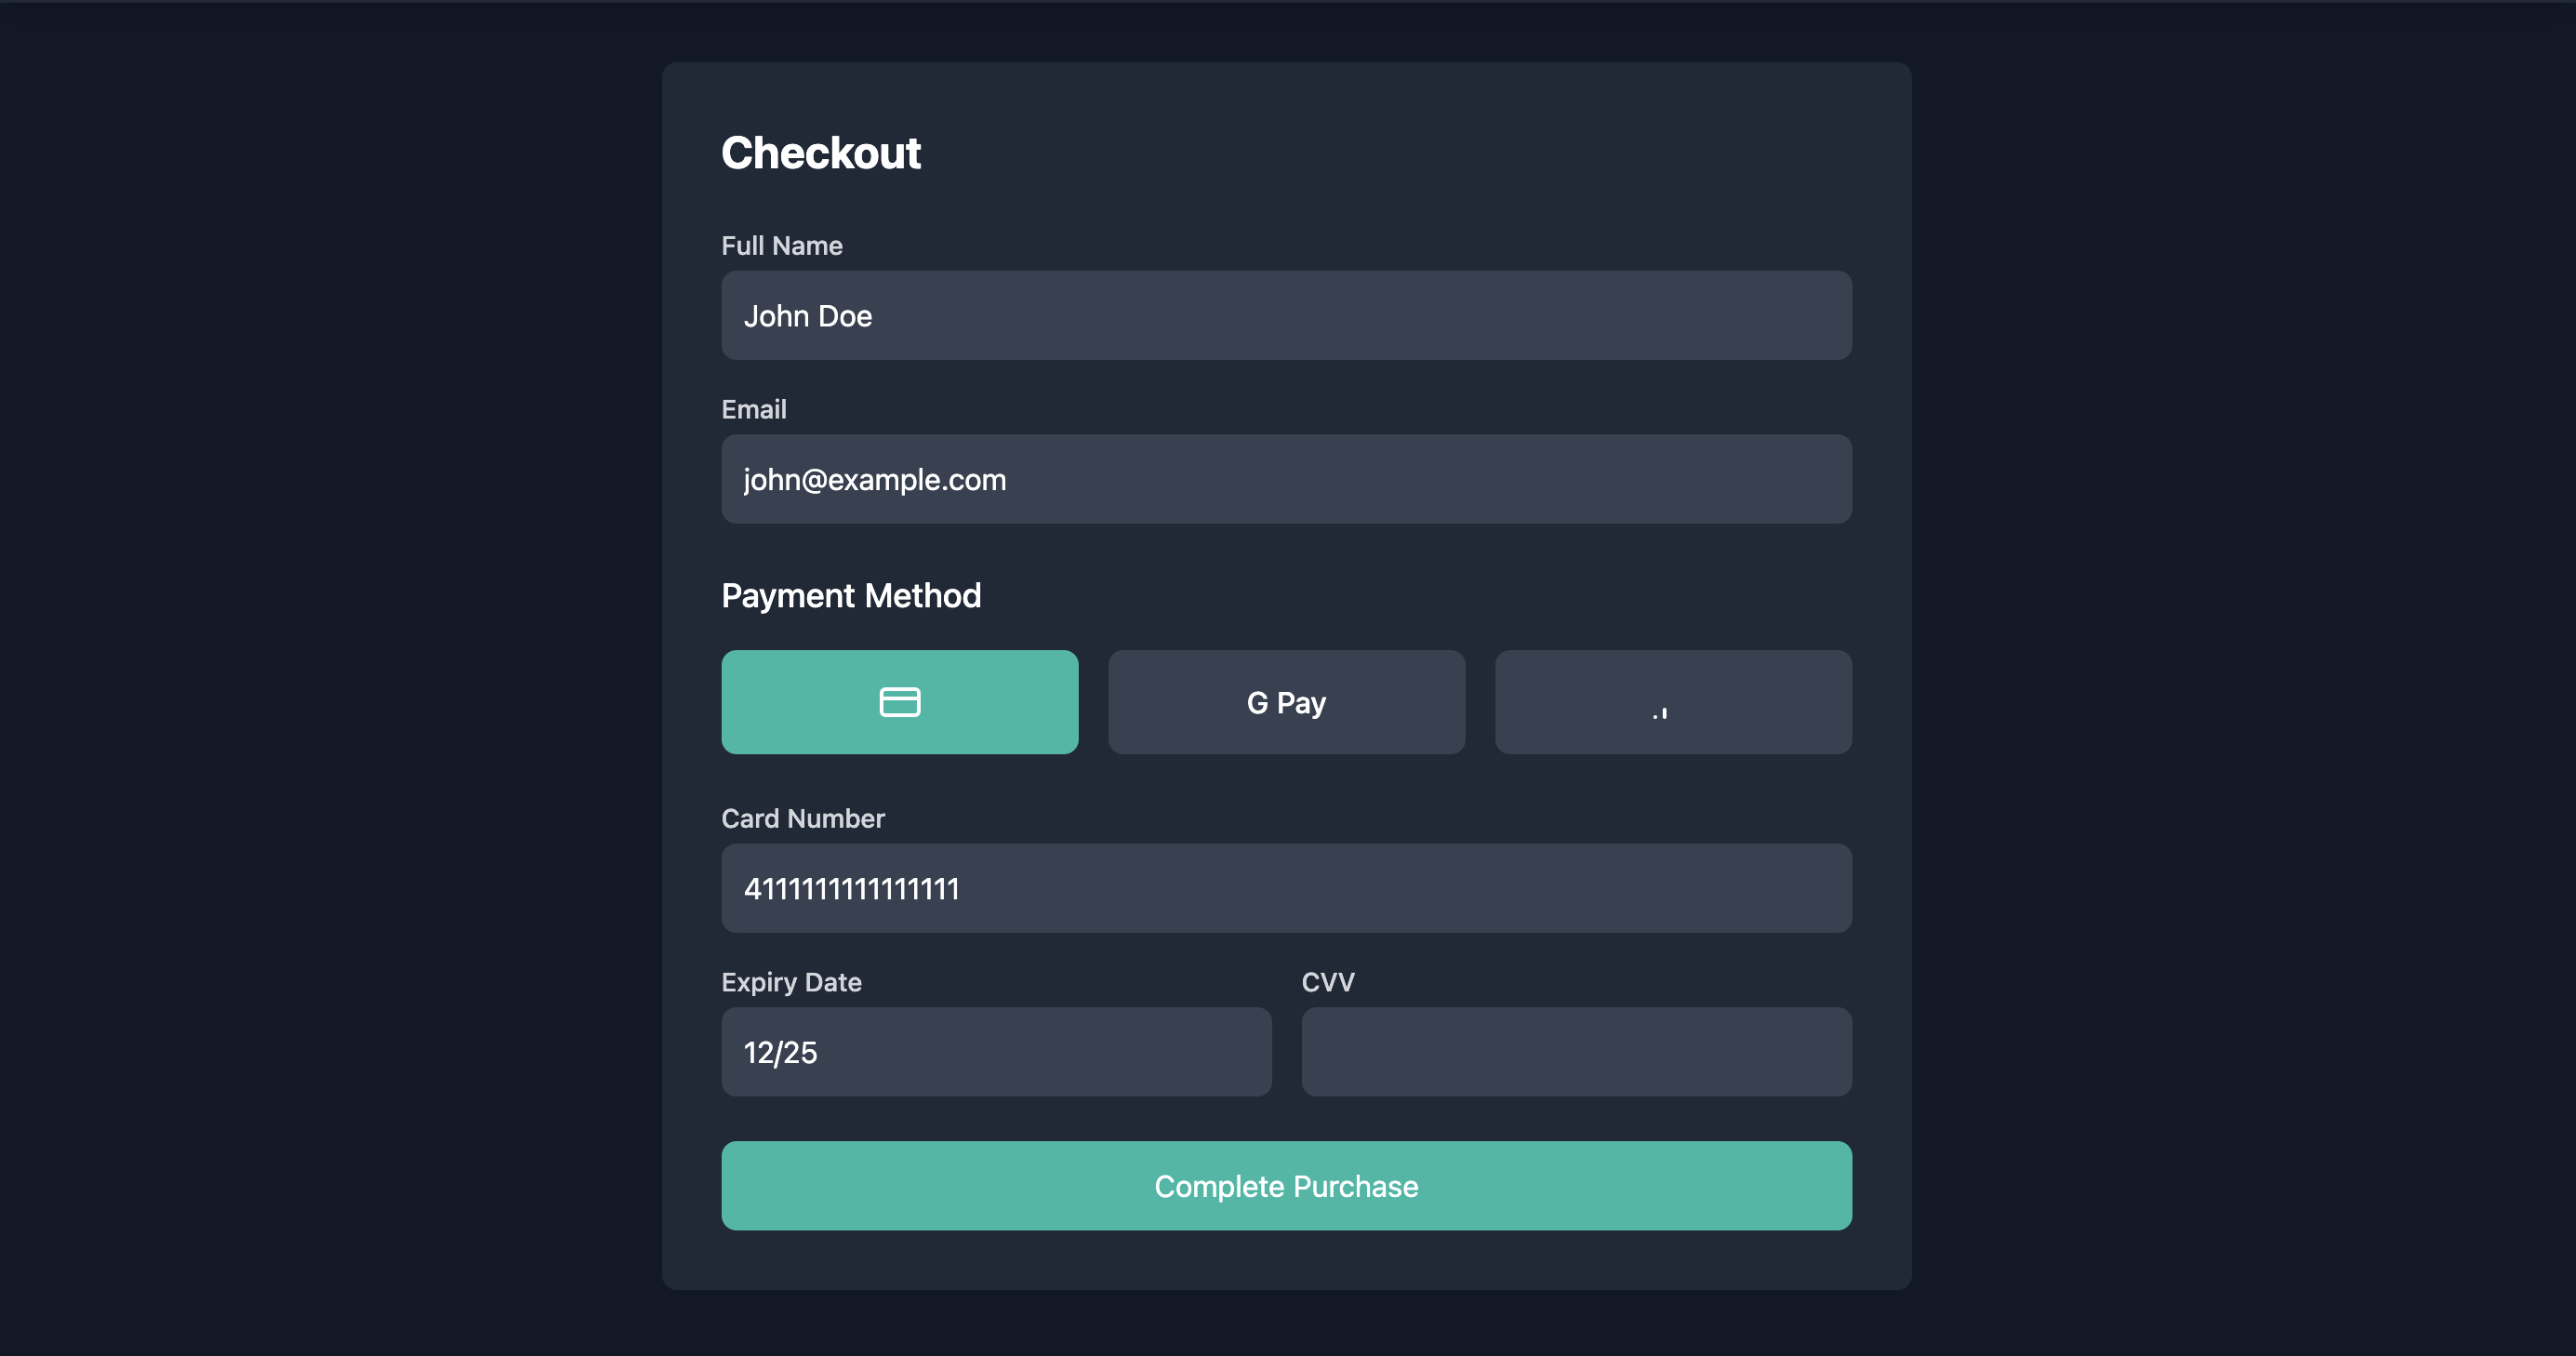
\includegraphics[width=0.9\textwidth]{Slike/FZ2ui/usercheckout.png}
    \caption{Prototip interfejsa za unos podataka o plaćanju za korisnika}
    \label{fig:usercheckout}
\end{figure}
\begin{figure}[H]
    \centering
    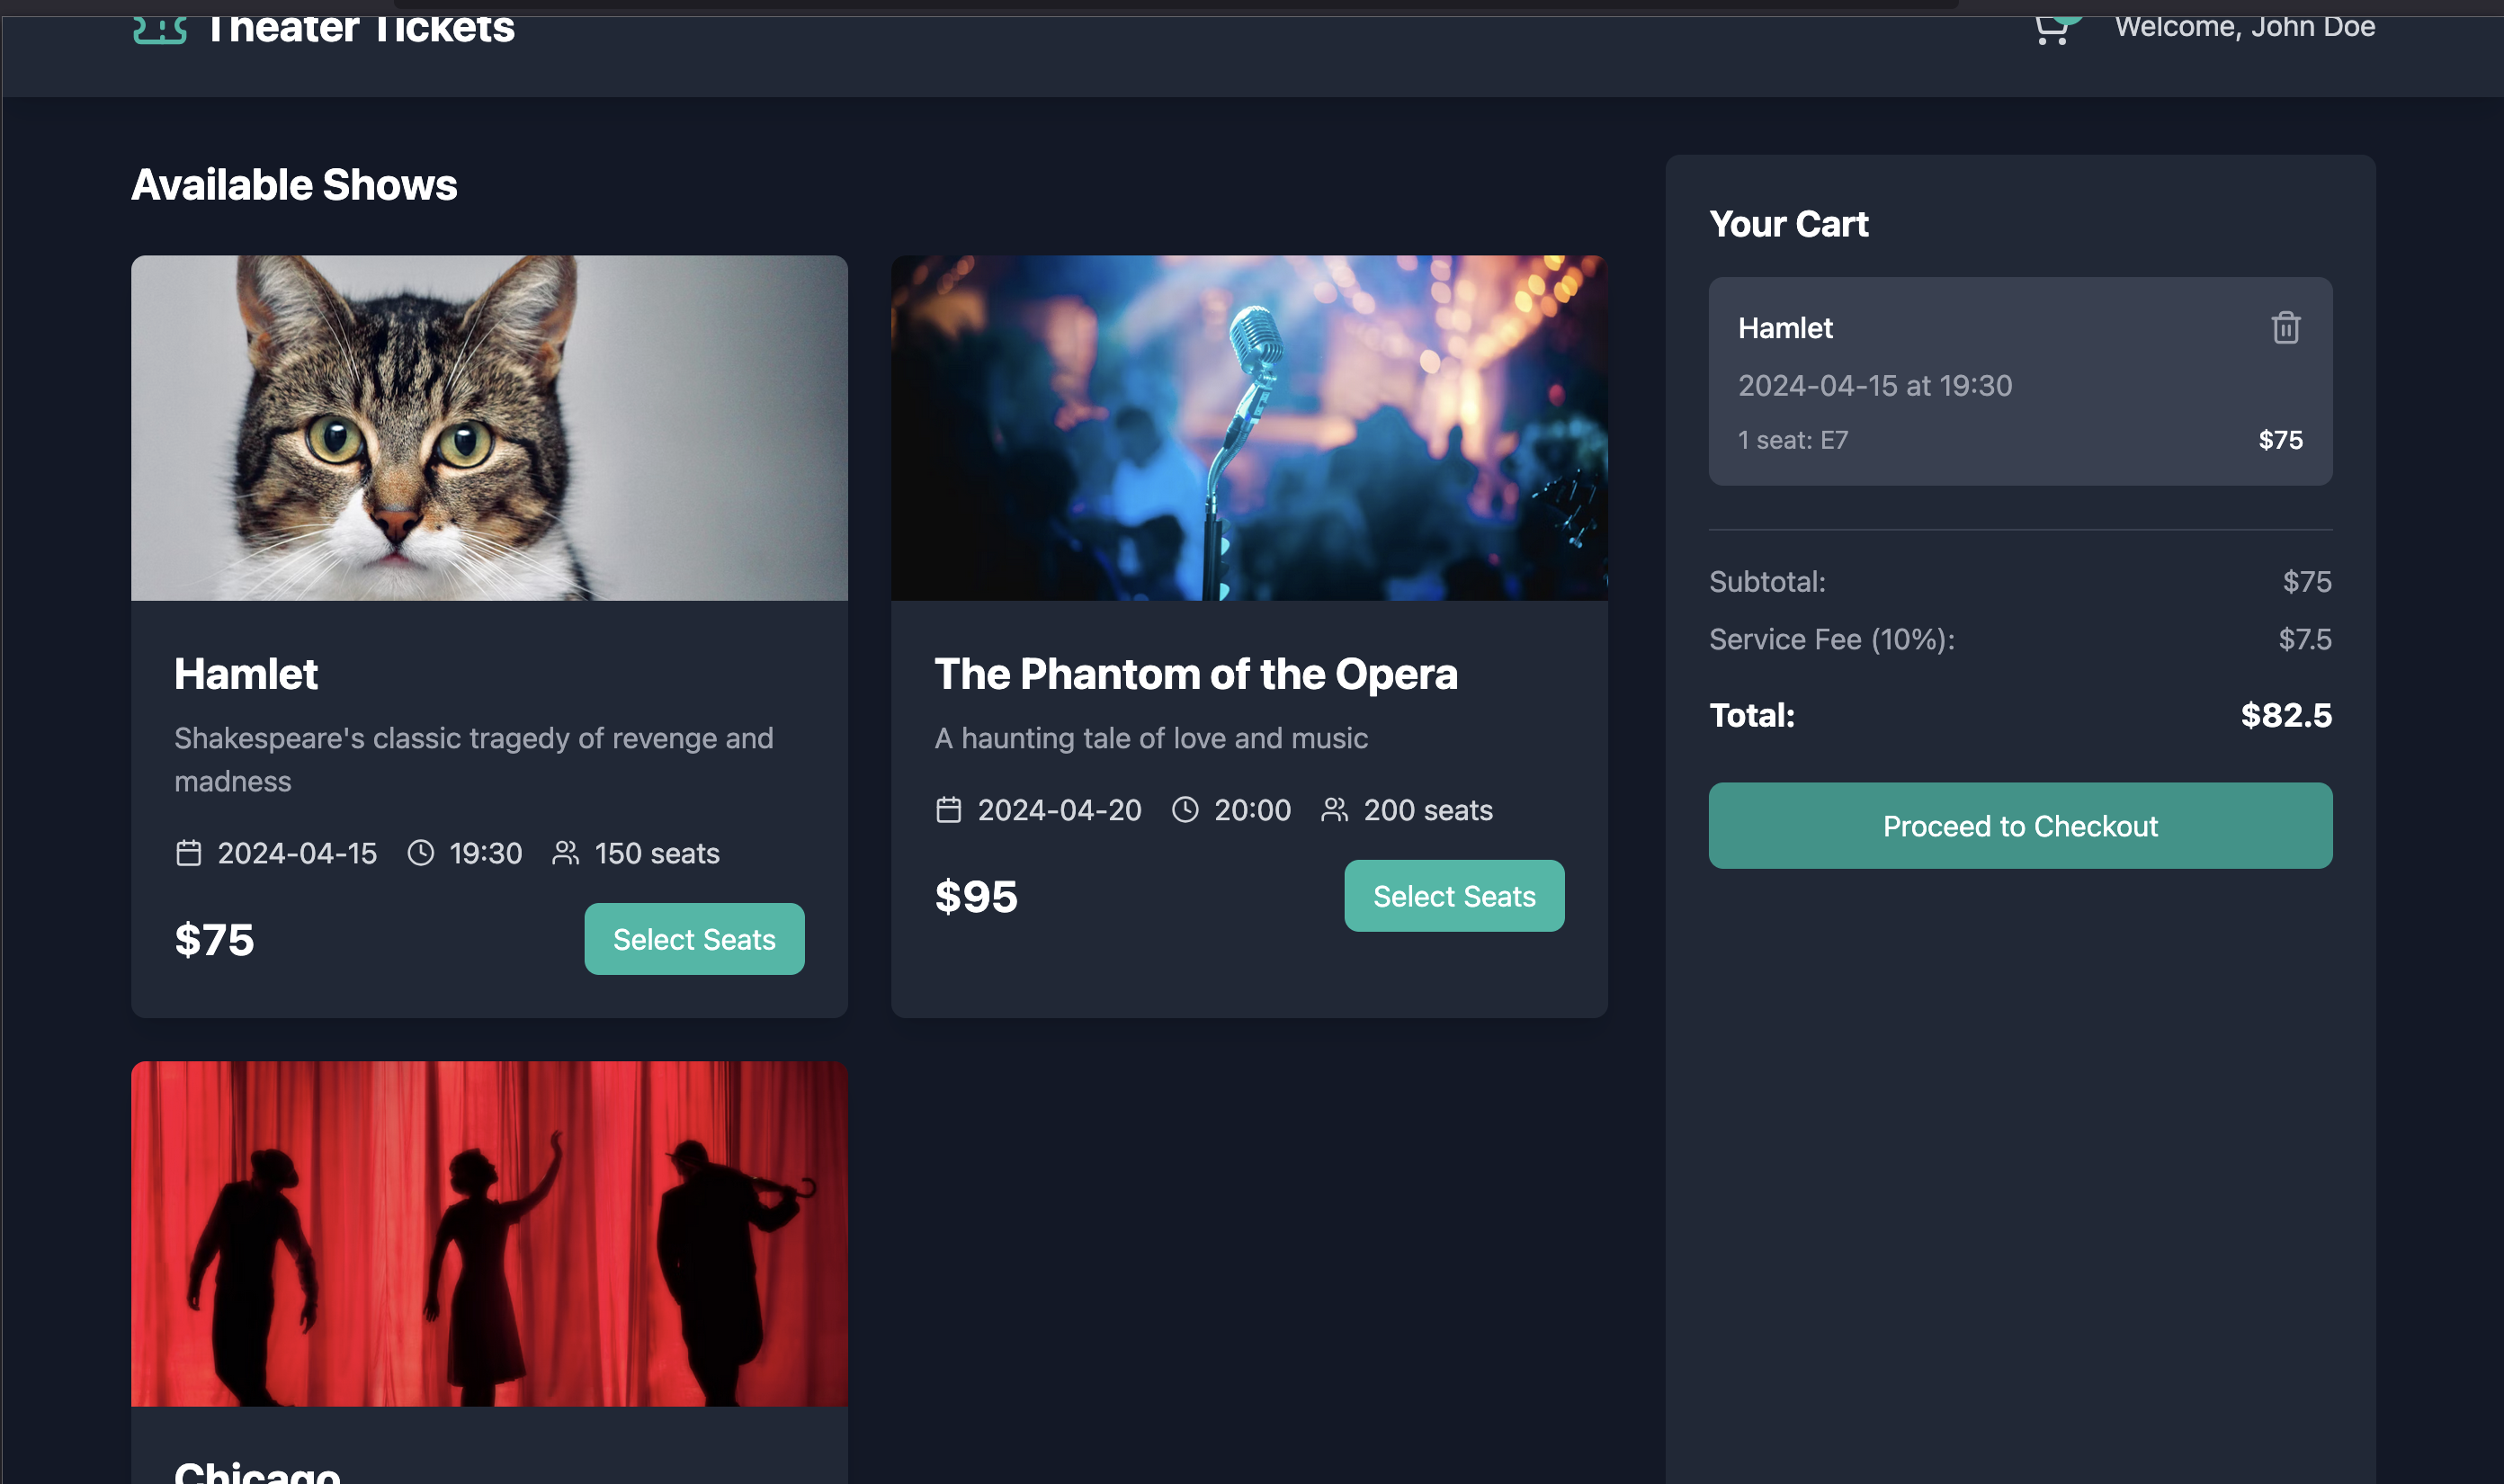
\includegraphics[width=0.9\textwidth]{Slike/FZ2ui/userfrontlist.png}
    \caption{Prototip interfejsa za prikaz korpe}
    \label{fig:userfrontlist}
\end{figure}
\begin{figure}[H]
    \centering
    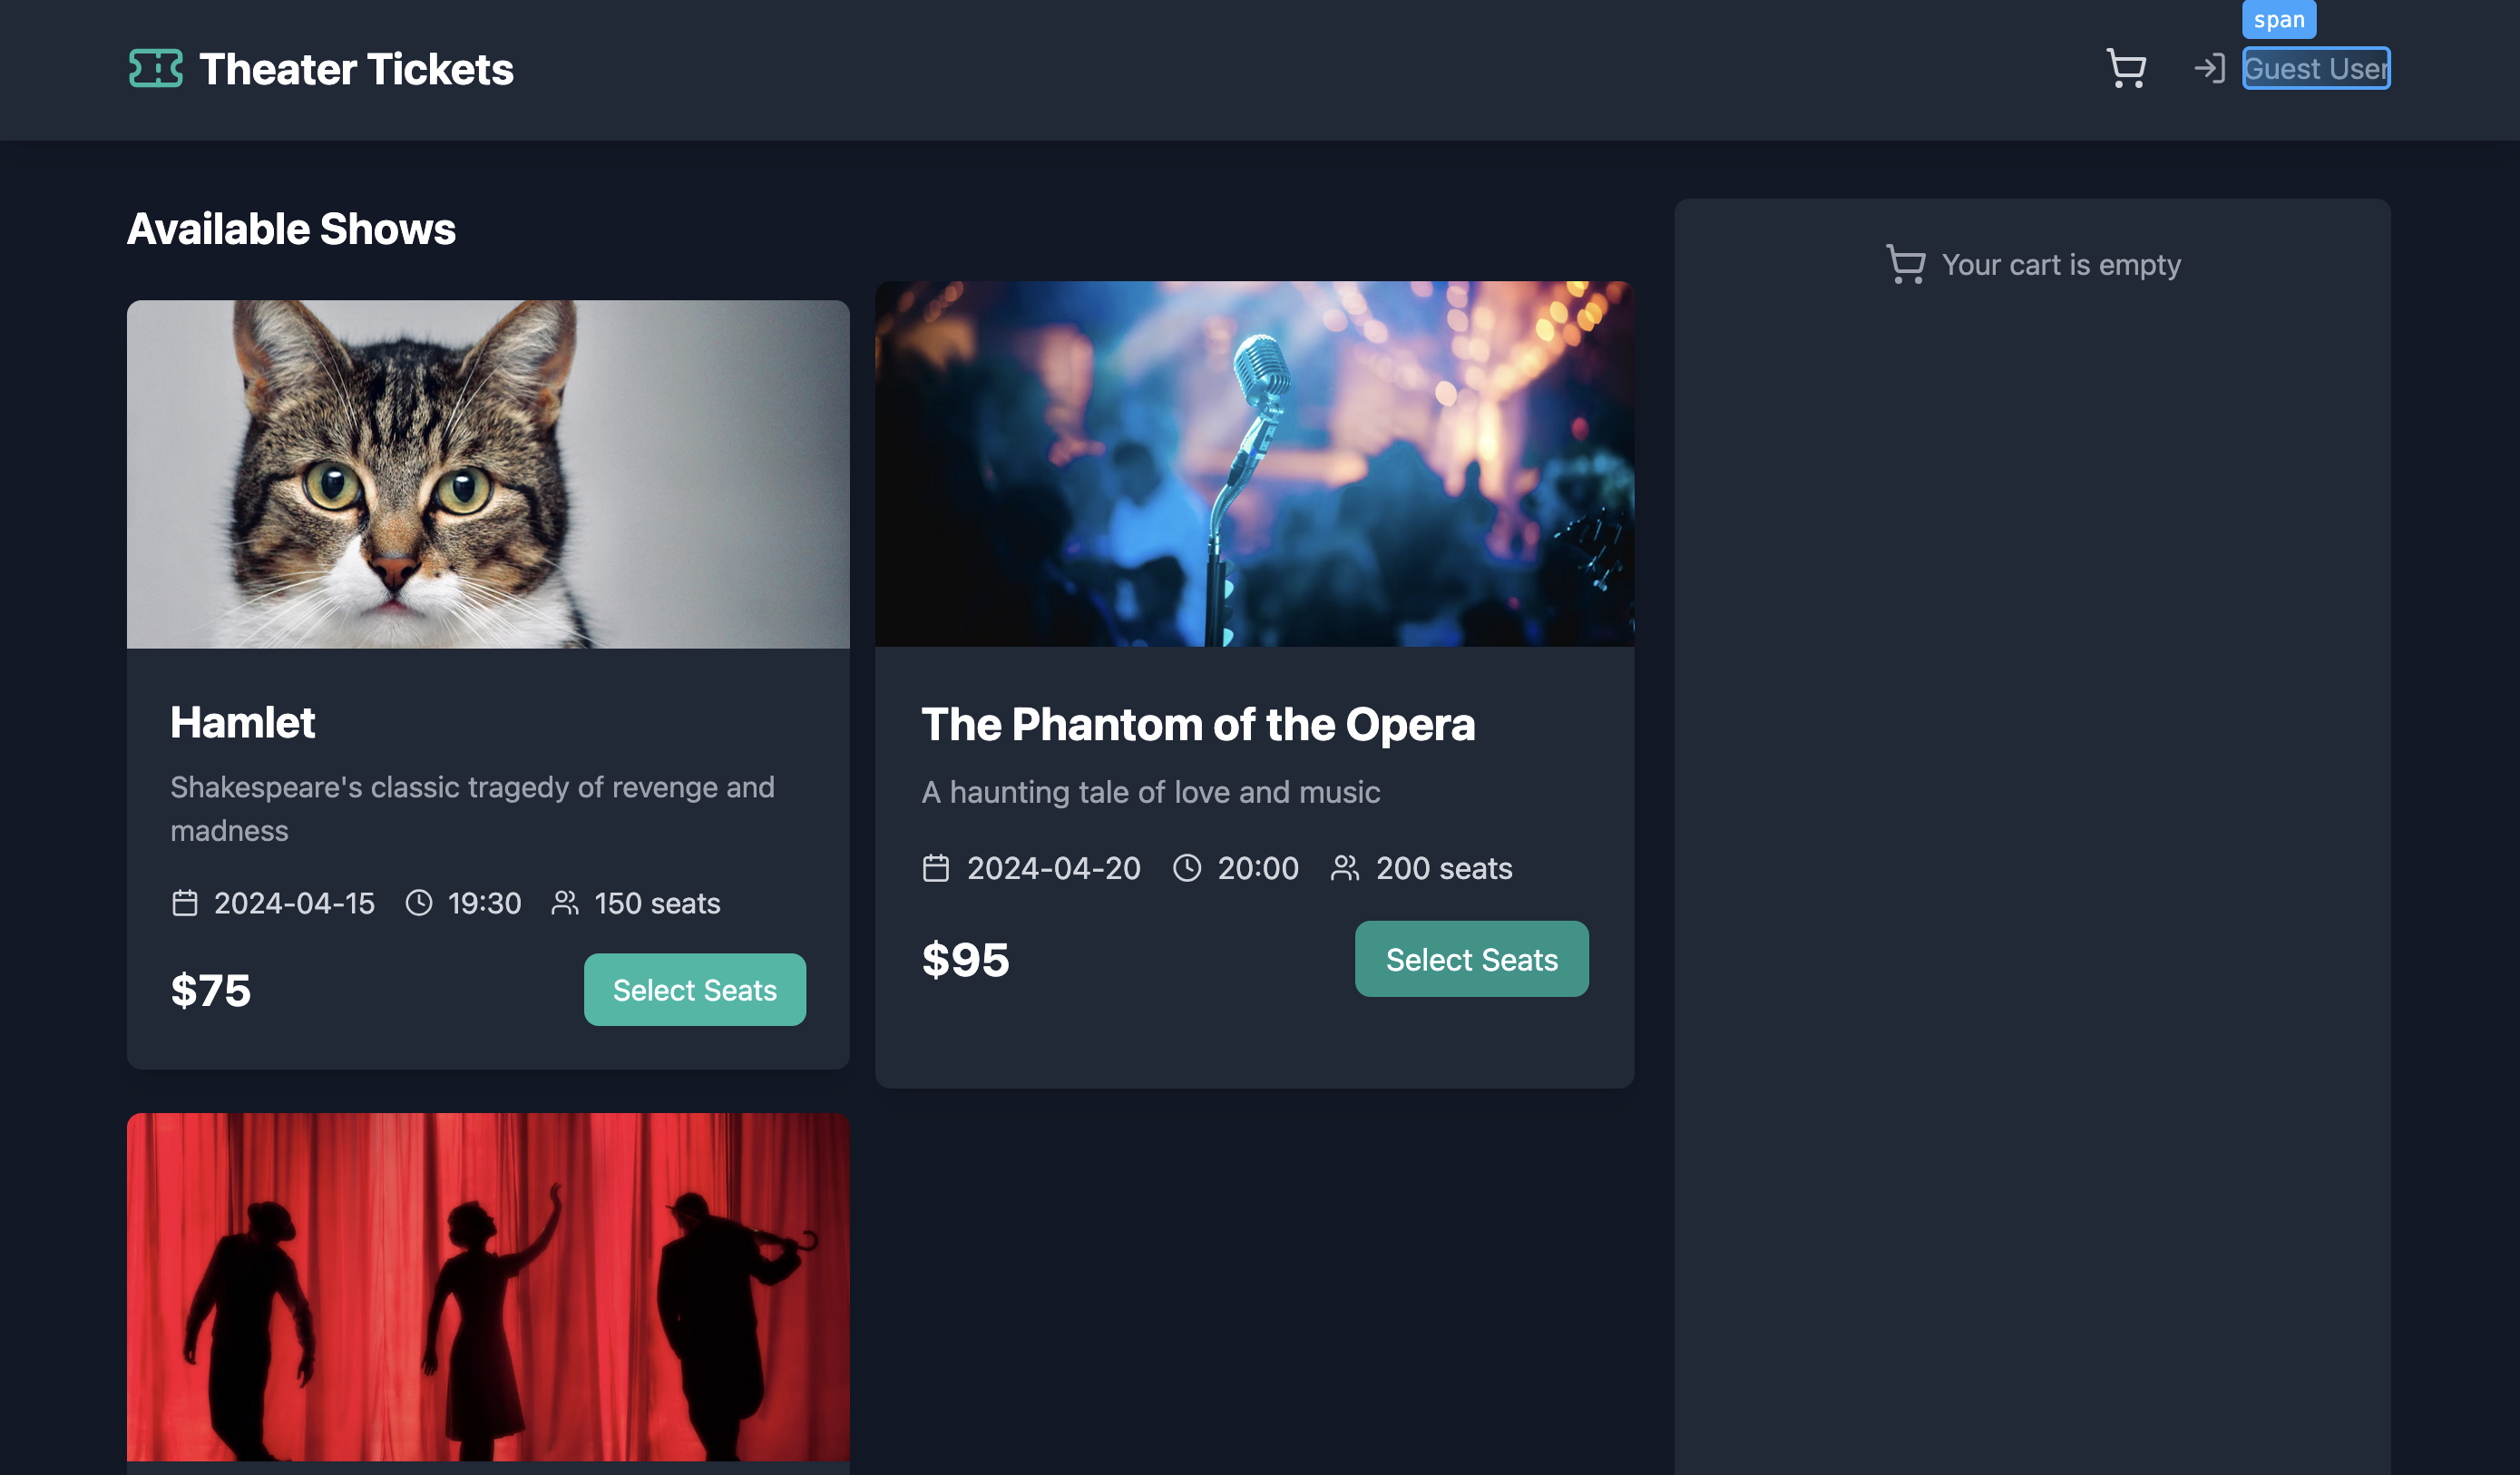
\includegraphics[width=0.9\textwidth]{Slike/FZ2ui/guesthome.png}
    \caption{Prototip interfejsa za prikaz predstava gostu}
    \label{fig:guesthome}
\end{figure}
\begin{figure}[H]
    \centering
    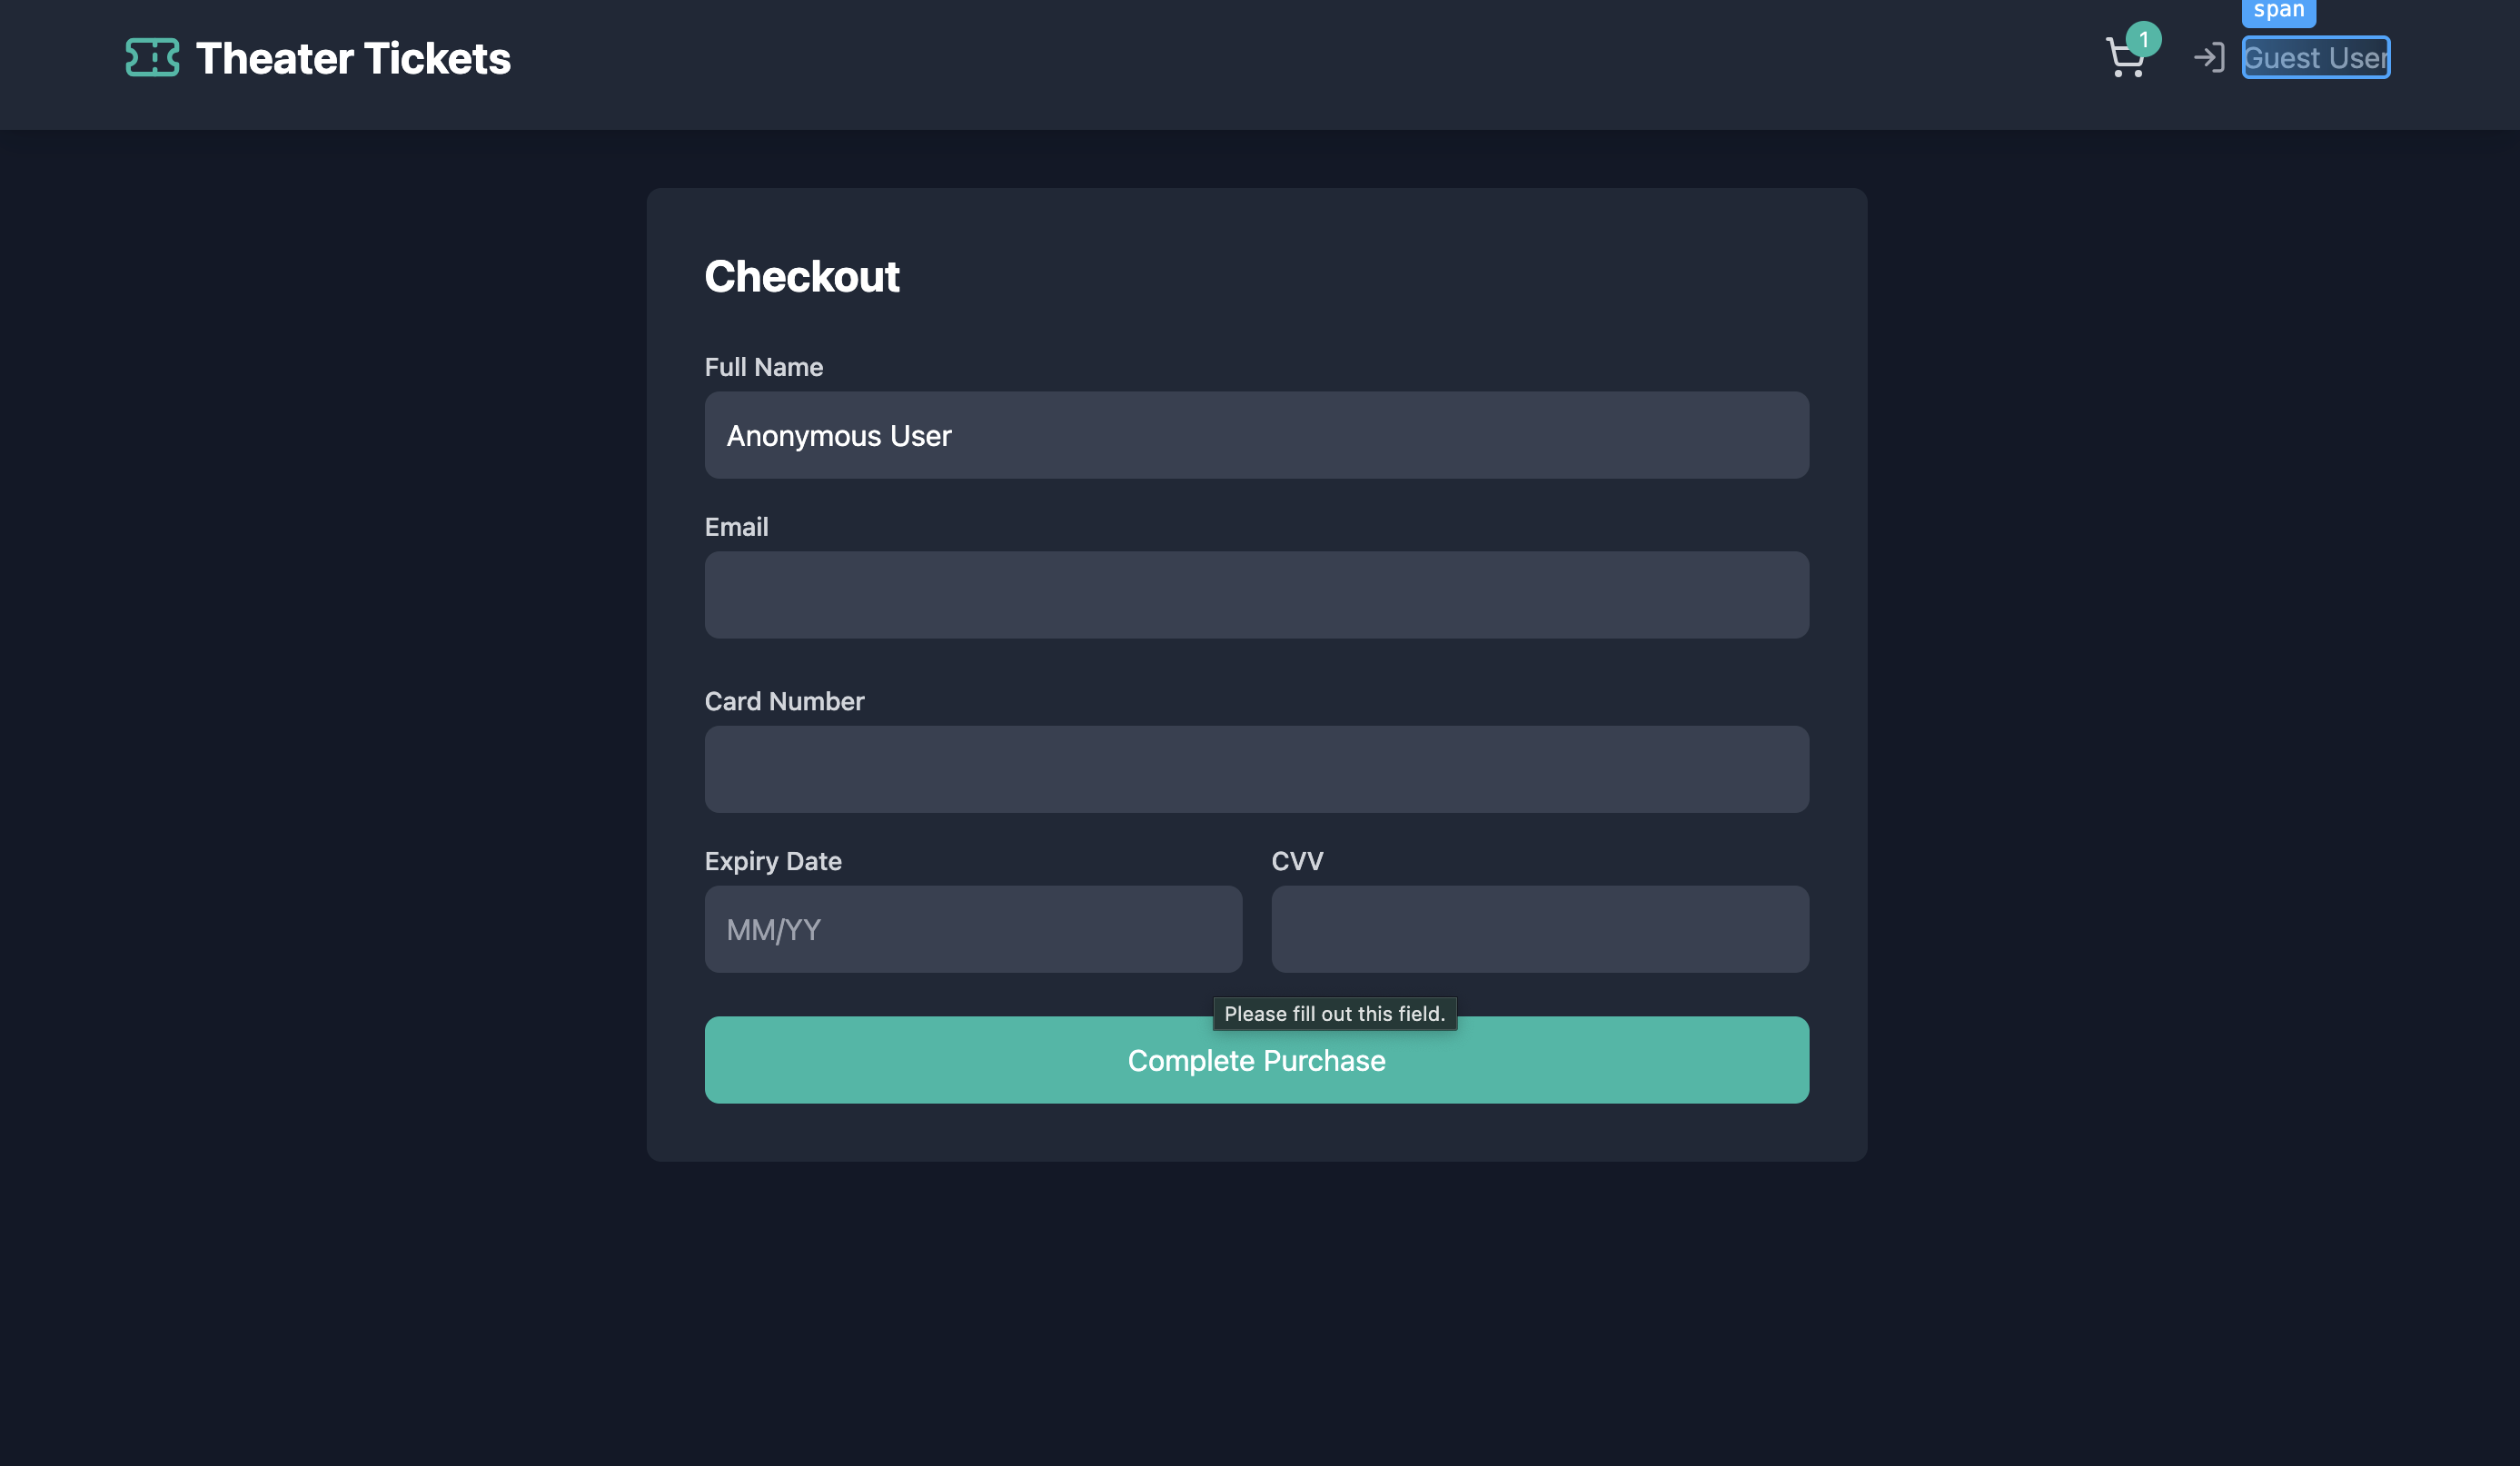
\includegraphics[width=0.9\textwidth]{Slike/FZ2ui/guestcheck.png}
    \caption{Prototip interfejsa za prikaz unosa podataka o plaćanju za neregistrovanog korisnika}
    \label{fig:questcheck}
\end{figure}
\subsection{Bolt promptovi}
\begin{enumerate}[itemsep=1ex]
    \item \textbf{Prvi \textit{prompt}:}

        \textit{ Create a modern and user friendly UI for ticket sales and reservation for a theatre. If the user is not registered he may view active plays, add one to his cart and checkout by filling out a reservation form. A registered user may view active plays, add them to his cart and checkout by choosing a method of payment: Credit Card, Google Pay, PayPal. If the registered user has already made purchases remember them and autofill the checkout. In all cases a message should be displayed for a successful reservation. Make the UI theme in dark mode.}

    \item \textbf{Drugi \textit{prompt}:}
        \begin{enumerate}[itemsep=0.5ex] 
            \item Homepage / Play Listing: \textit{Dark mode website homepage UI/UX design for a modern theater ticket sales platform. Features a clean grid layout of cards, each showing a high-quality theater play poster, title, and dates. Prominent call-to-action buttons in teal. Header includes logo, navigation links, cart icon, and login button. Overall professional and user-friendly aesthetic.}

            \item \textit{Play Details \& Seat Selection:}

            \textit{Modern dark mode UI/UX screen for theater seat selection. Shows an interactive seat map with a clear stage layout at the top. Seats are displayed in a grid, visually differentiated as available (grey), selected (teal accent color), and unavailable (dark grey/X). A sidebar displays selected seat details and total price. Clean, intuitive web application interface.}

            \textit{Alternative focus: Close-up on an interactive theater seat selection map UI element. Dark mode aesthetic, stage diagram at top, seats clearly marked as available, selected (teal highlight), and booked. Price calculation visible nearby. Modern web design.}

            \item \textit{Shopping Cart:}

            \textit{Dark mode shopping cart page UI/UX design for a theater ticket website. Displays a list of selected tickets, showing play title, date, time, seat numbers, quantity, and price per item. Each item has a 'Remove' option. Includes an order summary section calculating subtotal, fees, and total. A clear 'Proceed to Checkout' button uses a teal accent color. Clean and organized layout.}

            \item \textit{Checkout - Unregistered User:}

            \textit{Modern dark mode checkout screen UI/UX for an unregistered user on a theater ticket website. Features a simple reservation form with fields for Full Name, Email, and Phone Number. A clear order summary is visible (perhaps in a sidebar). A prominent 'Confirm Reservation' button uses a teal accent color. Minimalist and focused design.}

            \item \textit{Checkout - Registered User:}

            \textit{Modern dark mode checkout screen UI/UX for a registered user on a theater ticket website. Displays pre-filled user information (Name, Email). Features payment method selection with options for Credit Card (showing input fields for number, expiry, CVV), Google Pay (logo button), and PayPal (logo button). Order summary is clearly visible. A 'Pay Now' button uses a teal accent color. Professional and secure appearance.}

            \textit{Alternative focus:}

            \textit{UI/UX detail view of payment method selection on a dark mode checkout page. Shows radio buttons or distinct sections for Credit Card (with masked input fields), Google Pay logo, and PayPal logo. Teal accent color highlights selected option or buttons. Modern web interface.}

            \item \textit{Success Confirmation:}

            \textit{Dark mode success confirmation page UI/UX for a theater ticket purchase. Features a large, prominent checkmark icon in a teal accent color. A bold headline reads 'Reservation Confirmed!'. Includes a brief confirmation message mentioning email confirmation and order details recap. Buttons for 'View E-Tickets' or 'Back to Homepage'. Clean, positive, reassuring design.}
        \end{enumerate}

    \item \textbf{Treći \textit{prompt}:}
        \textit{Nothung you generated worked, can you re-do the design so you incorporate funcionalities as well?} Corrected typo \texttt{\textbackslash{}texit} -> \textit{\textbackslash{}textit}.

\end{enumerate}

\end{itemize}  

\sloppy  
\newpage
\section{FZ3: Korisnički profil}

\sloppy

\subsection{Opis funkcionalnog zahtjeva}

\begin{itemize}
    \item \textbf{Poslovni proces}: Korisnički profil.
    \item \textbf{Vrste korisnika}: Registrovani korisnik, Administrator.
    \item \textbf{Scenariji korištenja}:
    \begin{enumerate}
        \item \textbf{Registracija novog korisnika}: 

        
        Korisnik unosi svoje podatke (ime, prezime, e-mail, lozinka) u registracijski obrazac. Sistem provodi validaciju podataka i šalje verifikacijski e-mail korisniku. Nakon potvrde e-maila, korisnički račun se aktivira.
        
        \item \textbf{Ažuriranje korisničkog profila}: 

        
        Registrovani korisnik pristupa svom profilu putem stranice "Moj profil", gdje može ažurirati svoje osobne podatke, dodati ili promijeniti profilnu sliku te pregledati svoju povijest rezervacija i lojalne bodove.
        
        \item \textbf{Administratorski nadzor}: 

        
        Administrator ima pristup svim korisničkim profilima i može uređivati ili brisati korisničke račune prema potrebi, uz poštivanje sigurnosnih i privatnih smjernica.
    \end{enumerate}
    \item \textbf{UML dijagram aktivnosti}: Prikazani na slikama \ref{fig:fz3.1}, \ref{fig:fz3.2} i \ref{fig:fz3.12}
\end{itemize}

\begin{figure}[H]
    \centering
    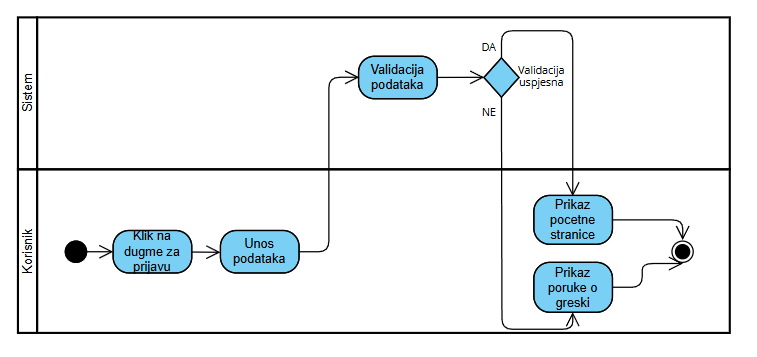
\includegraphics[width=0.9\textwidth]{Slike/fz3.1.png}
    \caption{UML dijagram aktivnosti "Korisnički profil"}
    \label{fig:fz3.1}
\end{figure}

\begin{figure}[H]
    \centering
    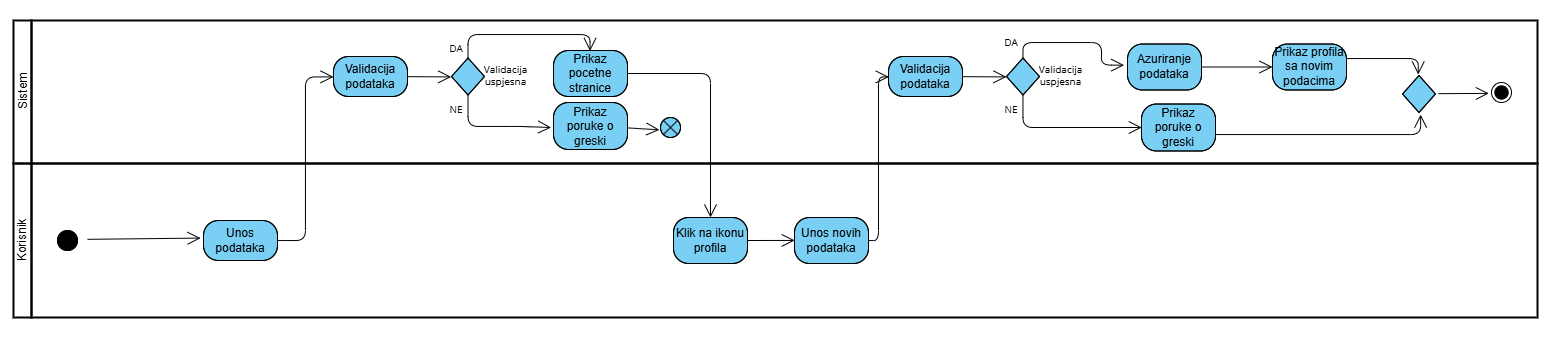
\includegraphics[width=0.9\textwidth]{Slike/fz3.2.png}
    \caption{UML dijagram aktivnosti "Uređivanje Korisničkog profila"}
    \label{fig:fz3.2}
\end{figure}

\begin{figure}[H]
    \centering
    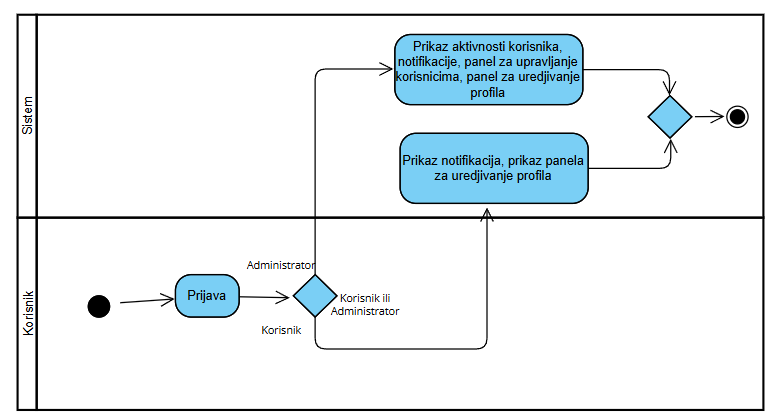
\includegraphics[width=0.9\textwidth]{Slike/fz3.12.png}
    \caption{UML dijagram aktivnosti "Aktivnosti aktera sistema"}
    \label{fig:fz3.12}
\end{figure}

\sloppy

\subsection{Dizajn korisničkih interfejsa}

\begin{itemize}
    \item \textbf{Prototip interfejsa}: Stranica za registraciju i prijavu, te stranica "Moj profil" s pregledom i uređivanjem korisničkih podataka. Demonstracija ovih funkcionalnosti je prikazana na slikama: \ref{fig:fz3.3}, \ref{fig:fz3.4}, \ref{fig:fz3.5}, \ref{fig:fz3.6}, \ref{fig:fz3.7}, \ref{fig:fz3.8}, \ref{fig:fz3.9}, \ref{fig:fz3.10}
    \item \textbf{Opis scenarija}:
    \begin{itemize}
        \item \textbf{Registracija korisnika}: 

        
        Korisnik pristupa stranici za registraciju, unosi svoje podatke i potvrđuje registraciju. Nakon toga, prima verifikacijski e-mail i aktivira svoj račun.
        
        \item \textbf{Prijava korisnika}: 

        
        Korisnik unosi svoje pristupne podatke (e-mail i lozinku) na stranici za prijavu. Ako su podaci ispravni, pristupa svom korisničkom profilu.
        
        \item \textbf{Ažuriranje profila}: 

        
        Na stranici "Moj profil", korisnik može pregledati i ažurirati svoje osobne podatke, dodati profilnu sliku i pregledati svoju povijest aktivnosti.
    \end{itemize}
\end{itemize}

\begin{figure}[H]
    \centering
    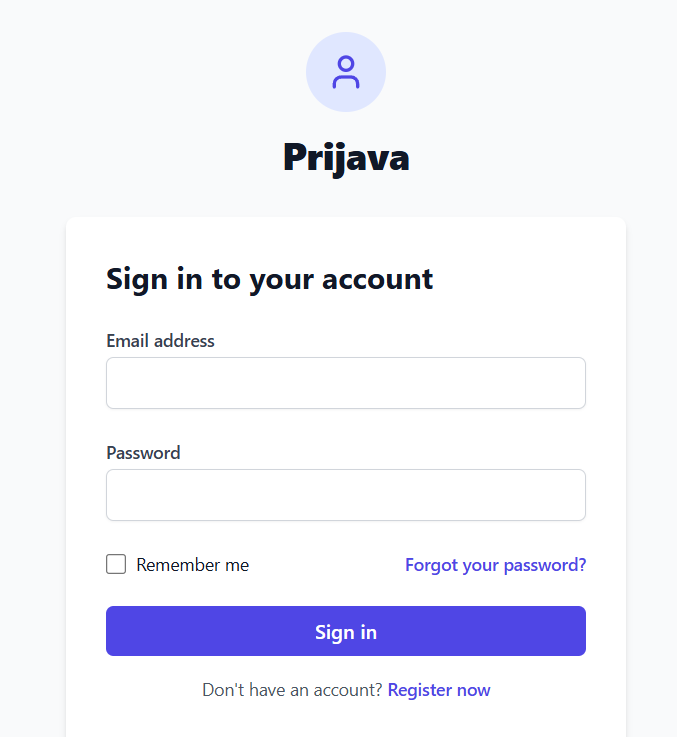
\includegraphics[width=0.9\textwidth]{Slike/fz3.3.png}
    \caption{Prototip stranice za prijavu korisnika}
    \label{fig:fz3.3}
\end{figure}

\begin{figure}[H]
    \centering
    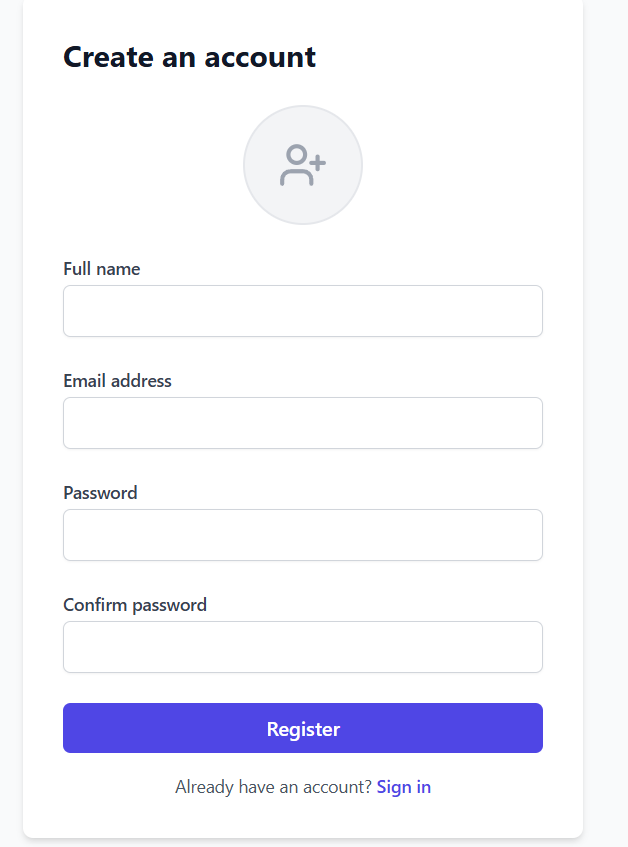
\includegraphics[width=0.9\textwidth]{Slike/fz3.4.png}
    \caption{Prototip stranice za registraciju korisnika}
    \label{fig:fz3.4}
\end{figure}

\begin{figure}[H]
    \centering
    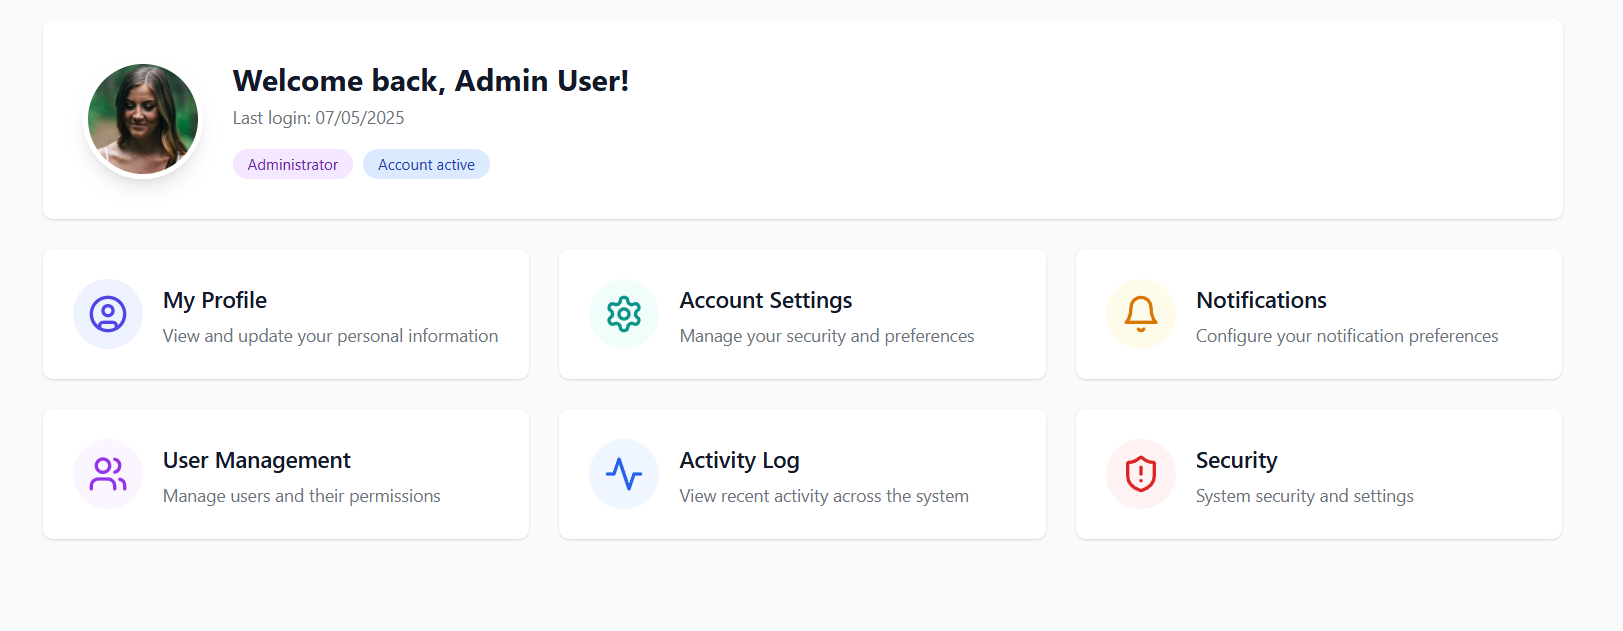
\includegraphics[width=0.9\textwidth]{Slike/fz3.5.png}
    \caption{Admin \textit{dashboard}}
    \label{fig:fz3.5}
\end{figure}

\begin{figure}[H]
    \centering
    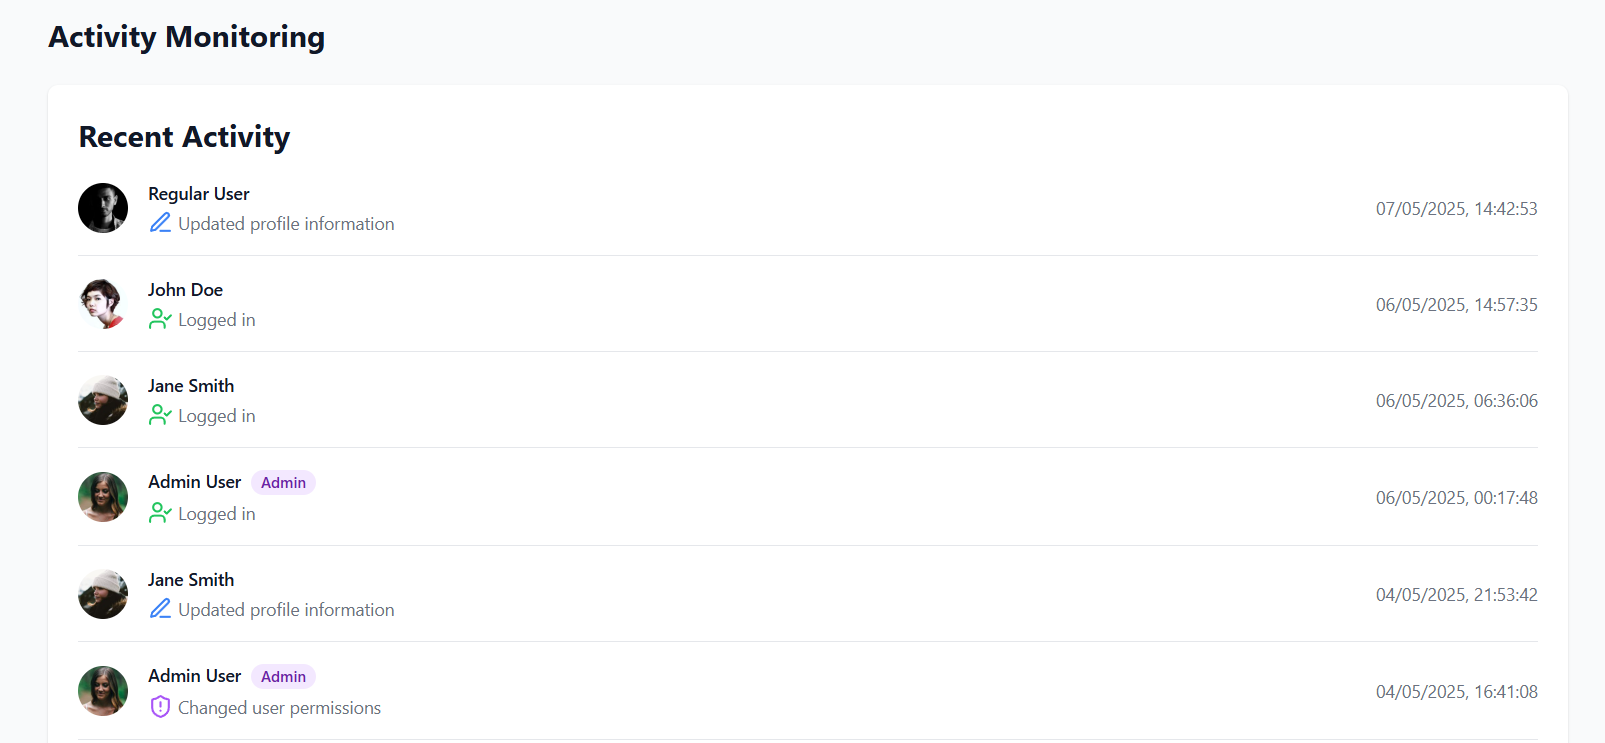
\includegraphics[width=0.9\textwidth]{Slike/fz3.6.png}
    \caption{Pregled aktivnosti korisnika}
    \label{fig:fz3.6}
\end{figure}

\begin{figure}[H]
    \centering
    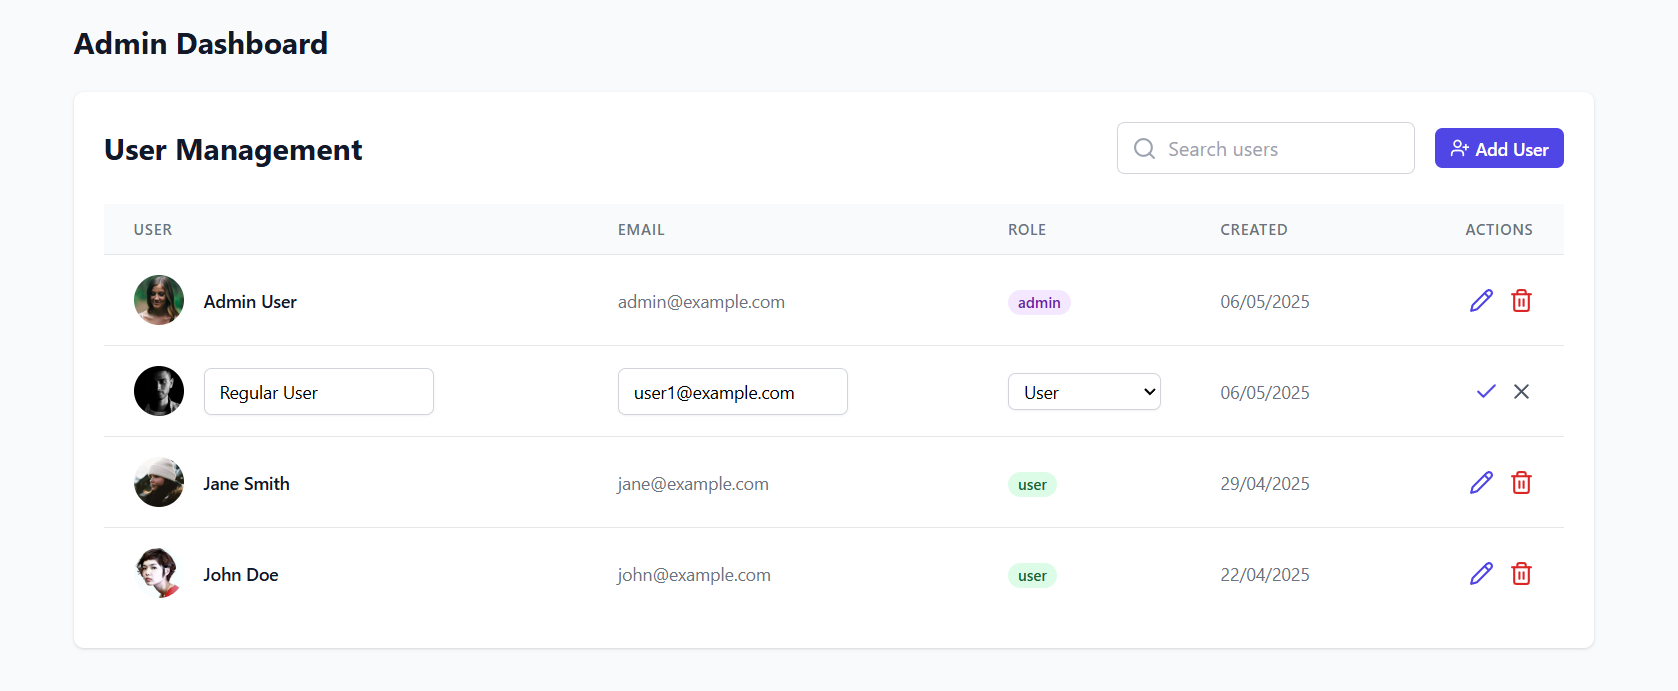
\includegraphics[width=0.9\textwidth]{Slike/fz3.7.png}
    \caption{Pregled svih korisnika i admina}
    \label{fig:fz3.7}
\end{figure}

\begin{figure}[H]
    \centering
    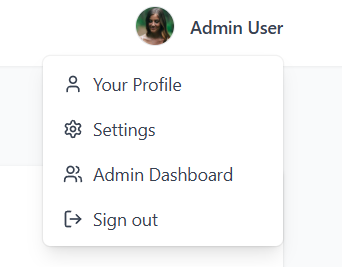
\includegraphics[width=0.9\textwidth]{Slike/fz3.8.png}
    \caption{Opcije dostupne adminima (korisnici nemaju opciju "Admin Dashboard")}
    \label{fig:fz3.8}
\end{figure}

\begin{figure}[H]
    \centering
    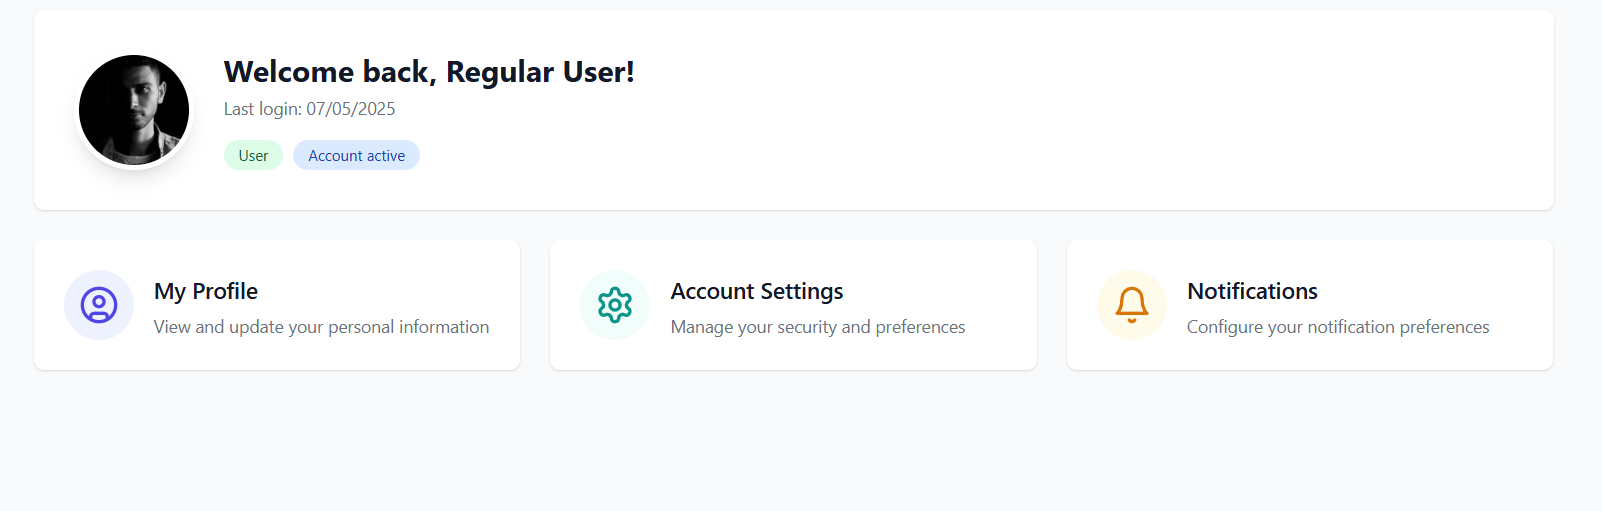
\includegraphics[width=0.9\textwidth]{Slike/fz3.9.png}
    \caption{Prikaz korisnikovog \textit{dashboard}-a}
    \label{fig:fz3.9}
\end{figure}

\begin{figure}[H]
    \centering
    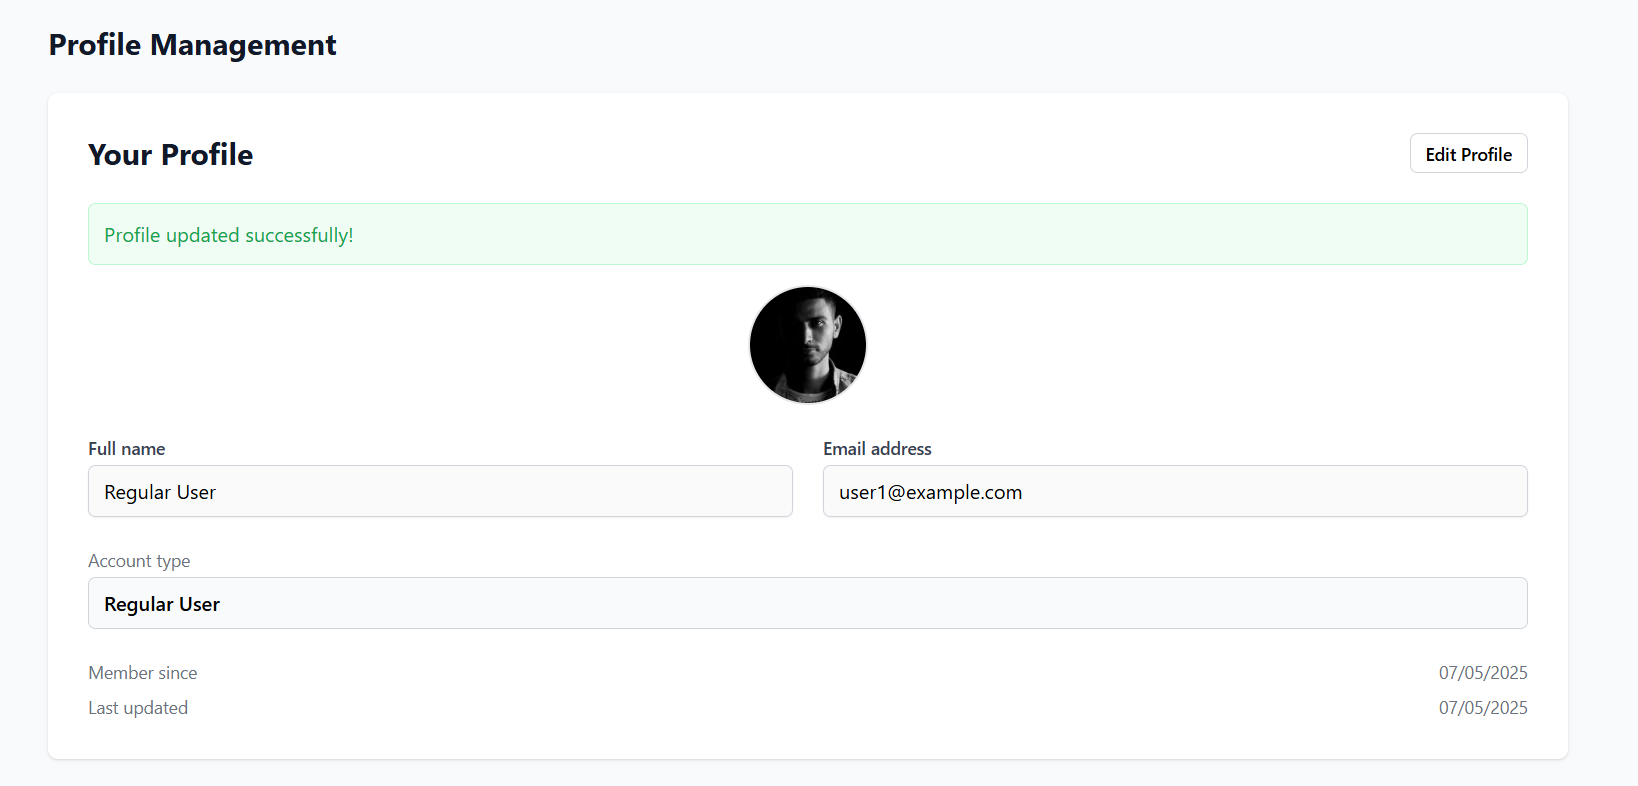
\includegraphics[width=0.9\textwidth]{Slike/fz3.10.png}
    \caption{Uređivanje profila}
    \label{fig:fz3.10}
\end{figure}

\subsection{Bolt \textit{prompt}-ovi}

\begin{enumerate}[itemsep=1ex]
    \item \textbf{Prvi \textit{prompt}:}

         \textit{Objective: Implement a comprehensive user profile management system that allows users to register, update, and manage their profiles, with administrative oversight.Functional Requirements:User Registration: Users must be able to create an account by providing necessary details such as name, email, password, and optional profile picture.Profile Updates: Users can update their personal information, including contact details, password, and preferences.Admin Controls: Administrators should have the ability to view, edit, or delete user profiles as necessary.Business Processes:User Registration:User accesses the registration page.User submits required information.System validates input and creates a new user account.Confirmation email sent to the user.Profile Management:User logs in and accesses their profile.User makes desired changes.System validates and saves changes.Confirmation of successful update displayed.Admin Oversight:Admin accesses user management dashboard.Admin views, edits, or deletes user profiles as needed.}
\end{enumerate}

\newpage  
\section{FZ4: Interaktivni forum}

\sloppy

\subsection{Opis funkcionalnog zahtjeva}

\begin{itemize}
    \item \textbf{Poslovni proces}:  Forum za predstave.
    \item \textbf{Vrste korisnika}: Registrovani korisnik, Gost (samo čitanje).
    \item \textbf{Scenariji korištenja}:
    \begin{enumerate}
        \item \textbf{Čitanje komentara i ocjena predstava}: 

        
        Gost ili registrovani korisnik može pristupiti forum stranici određene predstave i pregledavati sve prethodne komentare i ocjene koje su drugi korisnici ostavili.
        
        \item \textbf{Objava novog komentara}: 

        
        Registrovani korisnik odabire temu predstave na forumu, unosi svoj komentar ili ocjenu, i objavljuje je. Sistem bilježi vrijeme objave i povezuje komentar sa korisničkim nalogom.
    \end{enumerate}
    \item \textbf{UML dijagram aktivnosti}: Prikazan na slici \ref{fig:fz4}
\end{itemize}

\begin{figure}[H]
    \centering
    \includegraphics[width=1\textwidth]{Slike/Fz4.png}
    \caption{UML dijagram aktivnosti "Interaktivni forum"}
    \label{fig:fz4}
\end{figure}

\sloppy

\subsection{Dizajn korisničkih interfejsa}

\begin{itemize}
    \item \textbf{Prototip interfejsa}: Forum stranica sa listom tema za svaku predstavu, pregledom komentara, ocjenama i poljem za unos novog komentara (samo za registrovane korisnike). Prikazi prototipa interaktivnog foruma su dati na slikama: \ref{fig:fz4.3}, \ref{fig:fz4.4} i \ref{fig:fz4.5}
    \item \textbf{Opis scenarija}:
    \begin{itemize}
        \item \textbf{Dodavanje komentara}: 

        
        Registrovani korisnik odabire određenu predstavu, pristupa pripadajućoj temi na forumu, unosi komentar ili ocjenu i potvrđuje objavu.
        
        \item \textbf{Pasivno učešće gosta}: 

        
        Gost (neprijavljeni korisnik) može pregledavati sve forume i komentare, ali nema mogućnost dodavanja vlastitih komentara niti interakcije sa drugim korisnicima.
    \end{itemize}
\end{itemize}

\begin{figure}[H]
    \centering
    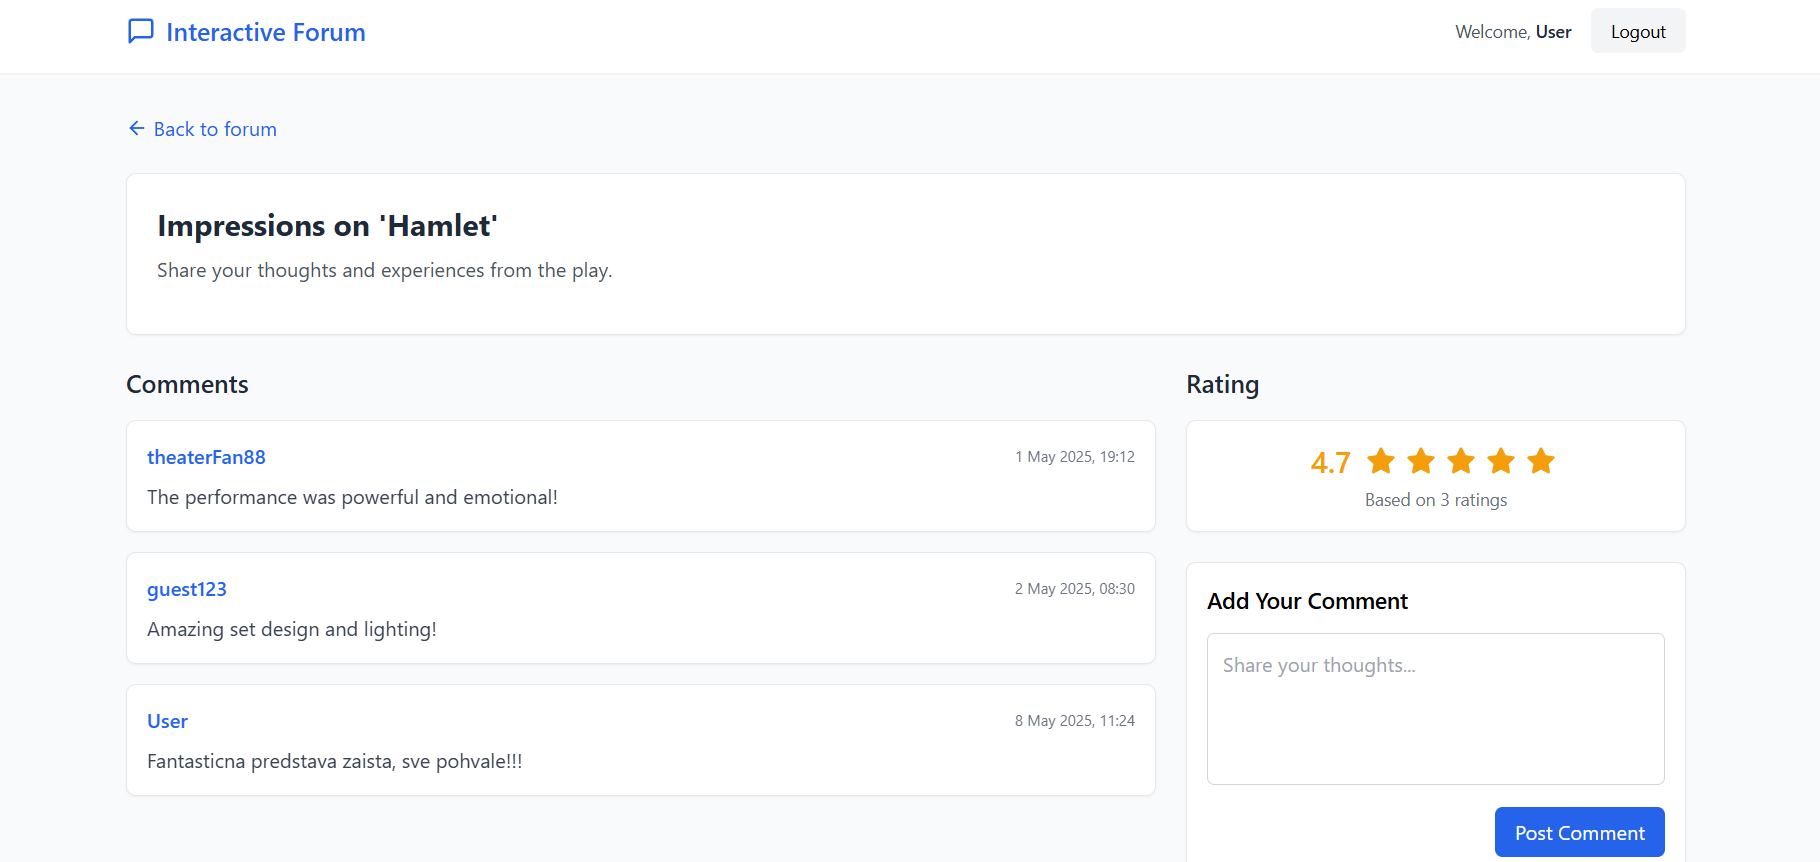
\includegraphics[width=0.9\textwidth]{Slike/fz4.3.png}
    \caption{Prikaz foruma za prijavljenog korisnika i ostavljena recenzija}
    \label{fig:fz4.3}
\end{figure}

\begin{figure}[H]
    \centering
    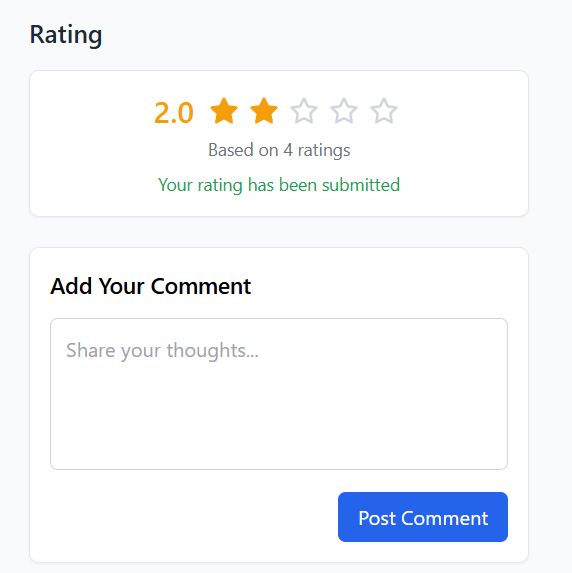
\includegraphics[width=0.9\textwidth]{Slike/fz4.4.png}
    \caption{Ostavljanje ocjene}
    \label{fig:fz4.4}
\end{figure}

\begin{figure}[H]
    \centering
    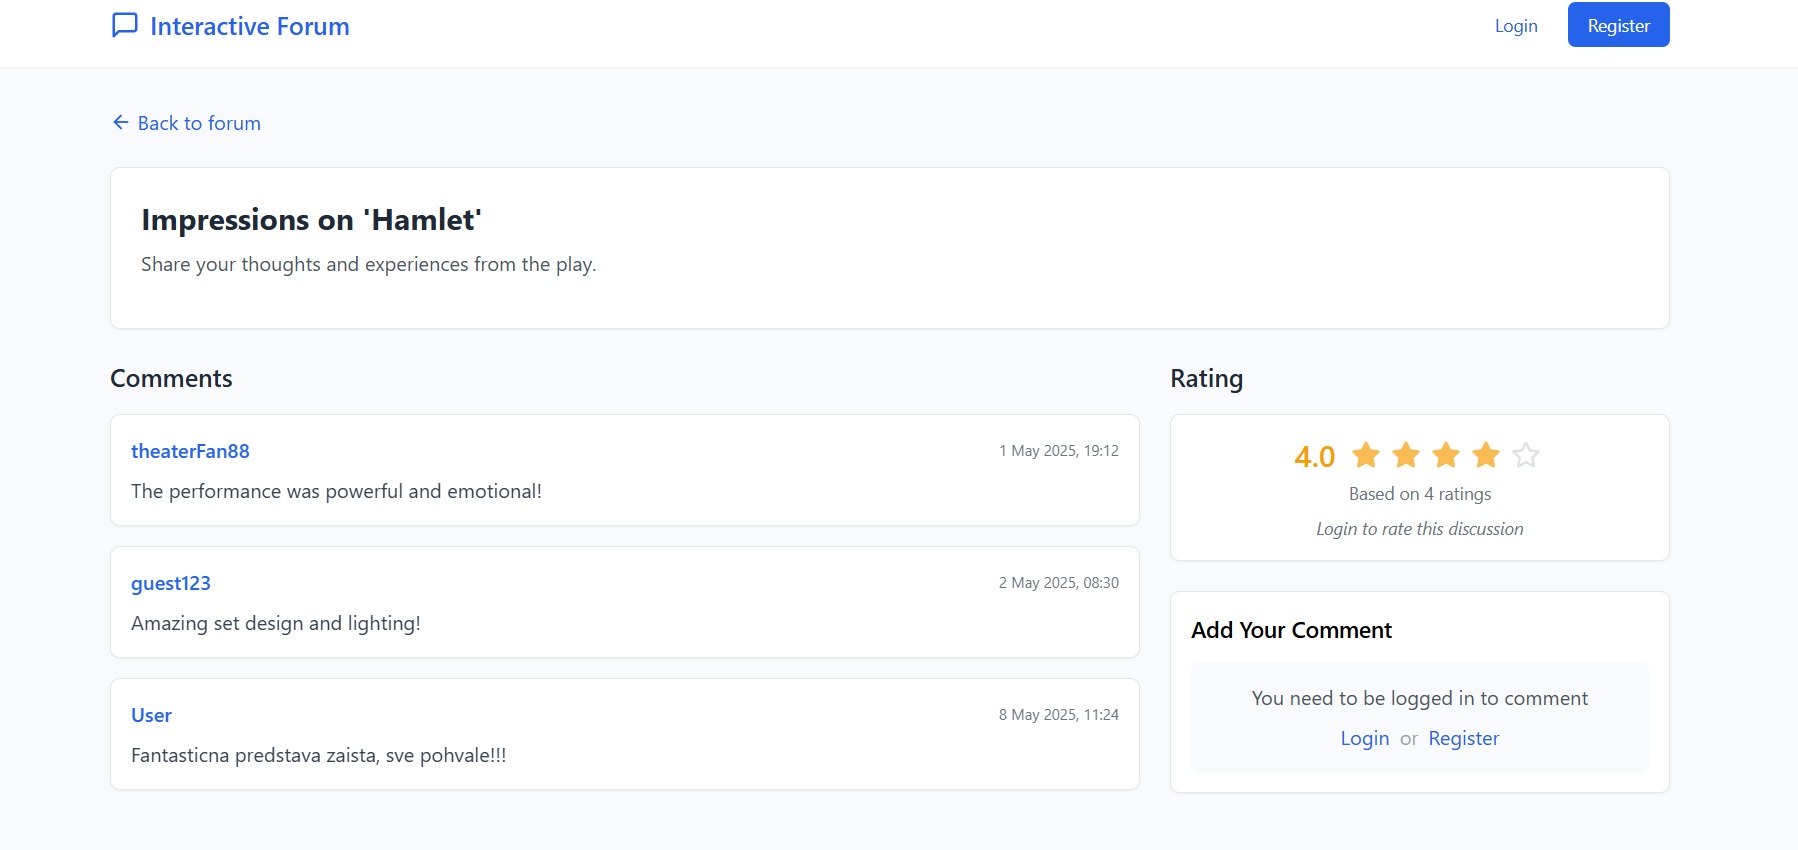
\includegraphics[width=0.9\textwidth]{Slike/fz4.5.png}
    \caption{Prikaz foruma za neprijavljenog korisnika - onemogućeno ostavljanje komentara}
    \label{fig:fz4.5}
\end{figure}

\begin{enumerate}[itemsep=1ex]
    \item \textbf{Prvi \textit{prompt}:}

         \textit{Objective: Develop an interactive forum where users can engage in discussions by posting and commenting, with different access levels for registered users and guests.Functional Requirements:Viewing Discussions: All users, including guests, can read existing forum threads and comments.Posting Comments: Registered users can post new comments in threads.Admin Moderation: Administrators can manage threads and comments, including deletion and reporting.Business Processes:Viewing Discussions:User accesses the forum page.System displays a list of threads with the number of comments.User selects a thread to view detailed comments.Posting Comments:Registered user logs in and selects a thread.User types and submits a comment.System validates and posts the comment.Confirmation of successful post displayed.Admin Moderation:Admin accesses the forum management dashboard.Admin reviews and manages threads and comments.System logs admin actions for auditing purposes.User Types:Registered Users: Can post comments and participate in discussions.Guests: Can only view threads and comments; cannot post.Administrators: Can manage all aspects of the forum.Usage Scenarios:Scenario 1: A guest reads through a discussion thread without posting.Scenario 2: A registered user logs in, posts a comment, and receives confirmation.Scenario 3: An administrator moderates a thread by deleting inappropriate comments.User Interface Design:Forum Page:List of discussion threads with titles and comment counts about theatre plays.Pagination or infinite scroll for thread navigation.Search bar to filter threads by keywords.Thread View:Display of original post and subsequent comments.Input field for registered users to submit new comments."Post Comment" button to submit.Admin options to delete or report comments.}
\end{enumerate}


\pagebreak
\sloppy  
\section{FZ5: Integracija društvenih mreža}  

\sloppy  
\subsection{Opis funkcionalnog zahtjeva}  
\begin{itemize}  
    \item \textbf{Poslovni proces}: Marketing i korisnička podrška  
    \item \textbf{Vrste korisnika}: Korisnik  
    \item \textbf{Scenariji korištenja}:  
        \begin{enumerate}  
            \item \textbf{Korisnik je povezao profil i objavio generisanu sliku}

            Nakon pritiska za dijeljenje predstave, generiše se slika. Korisnik je ili već povezao profil ili naknadno veže profil prijavom, te dijeli objavu.
            
            \item \textbf{Korisnik je povezao profil i objavio preuređenu sliku}

            Korisnik prije objave preuređuje sliku, promjenom stila ili slike.
            
            \item \textbf{Korisnik nije povezao profil i odustao od objave}

            Korisnik odustaje od objave, nakon zahtjeva za povezivanje profila.
            
        \end{enumerate}  
    \item \textbf{UML dijagram aktivnosti}: Prikazan na slici \ref{fig:fz5UML} 
\begin{figure}[H]
    \centering
    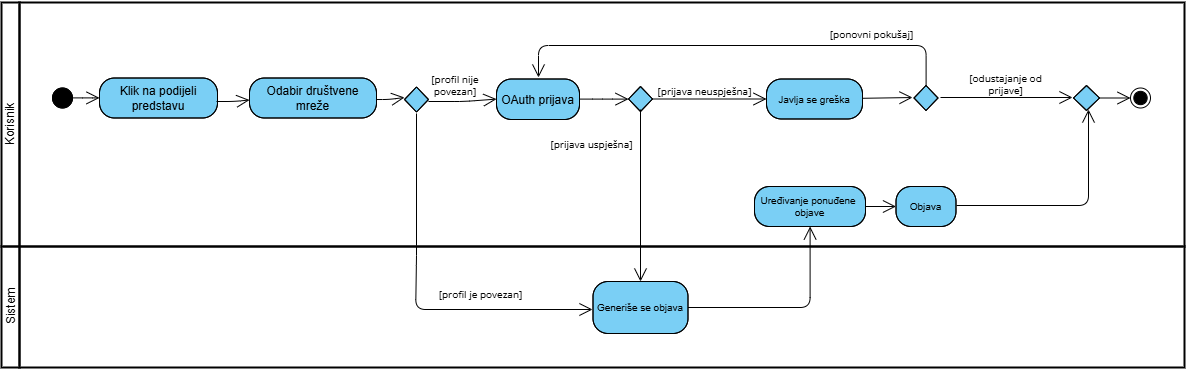
\includegraphics[width=1\linewidth]{Slike/FZ5/allmyhomieshatevpd.png}
    \caption{UML dijagram za integraciju društvenih mreža}
    \label{fig:fz5UML}
\end{figure}
    \item \textbf{Opis scenarija}:  
        \begin{itemize}  
            \item Korisnik klikne na dugme za dijeljenje putem zadane platforme  
            
            \item Ukoliko nije povezan profil traži se prijava putem \textit{OAuth}-a

            \item Nakon uspješno povezanog profila se generiše \textit{preview} za objavu, ukoliko se odustane od povezivanja, korisnik se vraća

            \item Objavu je moguće preurediti

            \item Dijeljenje objave
        \end{itemize}  
\end{itemize}  

\sloppy  
\subsection{Dizajn korisničkih interfejsa}  
\begin{itemize}  
    \item \textbf{Prototip interfejsa}: Na slici \ref{fig:shareplayoverview} moežemo da vidimo opcije dijeljenja predstava putem \textit{Instagram}-a i \textit{TikTok}-a. Ukoliko korisnik nije povezao profil javlja se poruka sa slike \ref{fig:connecttitktok}. Slika \ref{fig:preview} prikazuje generisanu sliku za objavu, koju je moguće preurediti promjenom slike ili stila, što vidimo na slici \ref{fig:previewchange}.

    \begin{figure}[H]
        \centering
        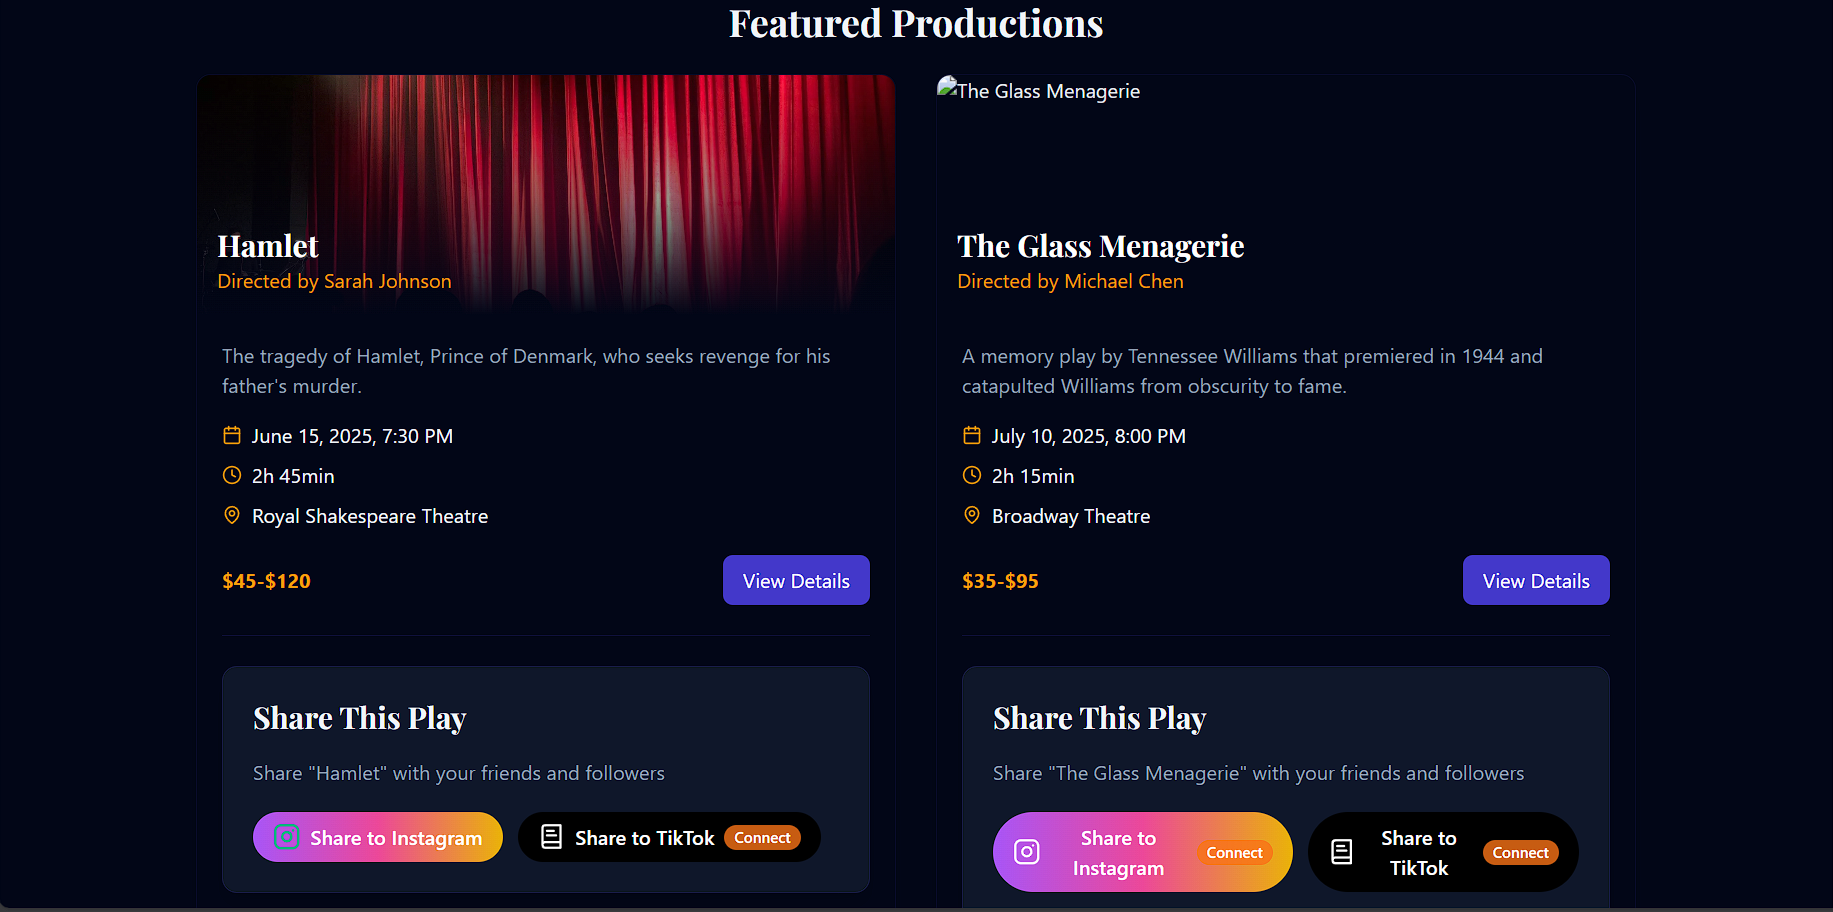
\includegraphics[width=\linewidth]{Slike/FZ5/shareplayoverview.png}
        \caption{Primjer pregleda predstava sa opcijama dijeljenja sadržaja}
        \label{fig:shareplayoverview}
    \end{figure}

    \begin{figure}[H]
        \centering
        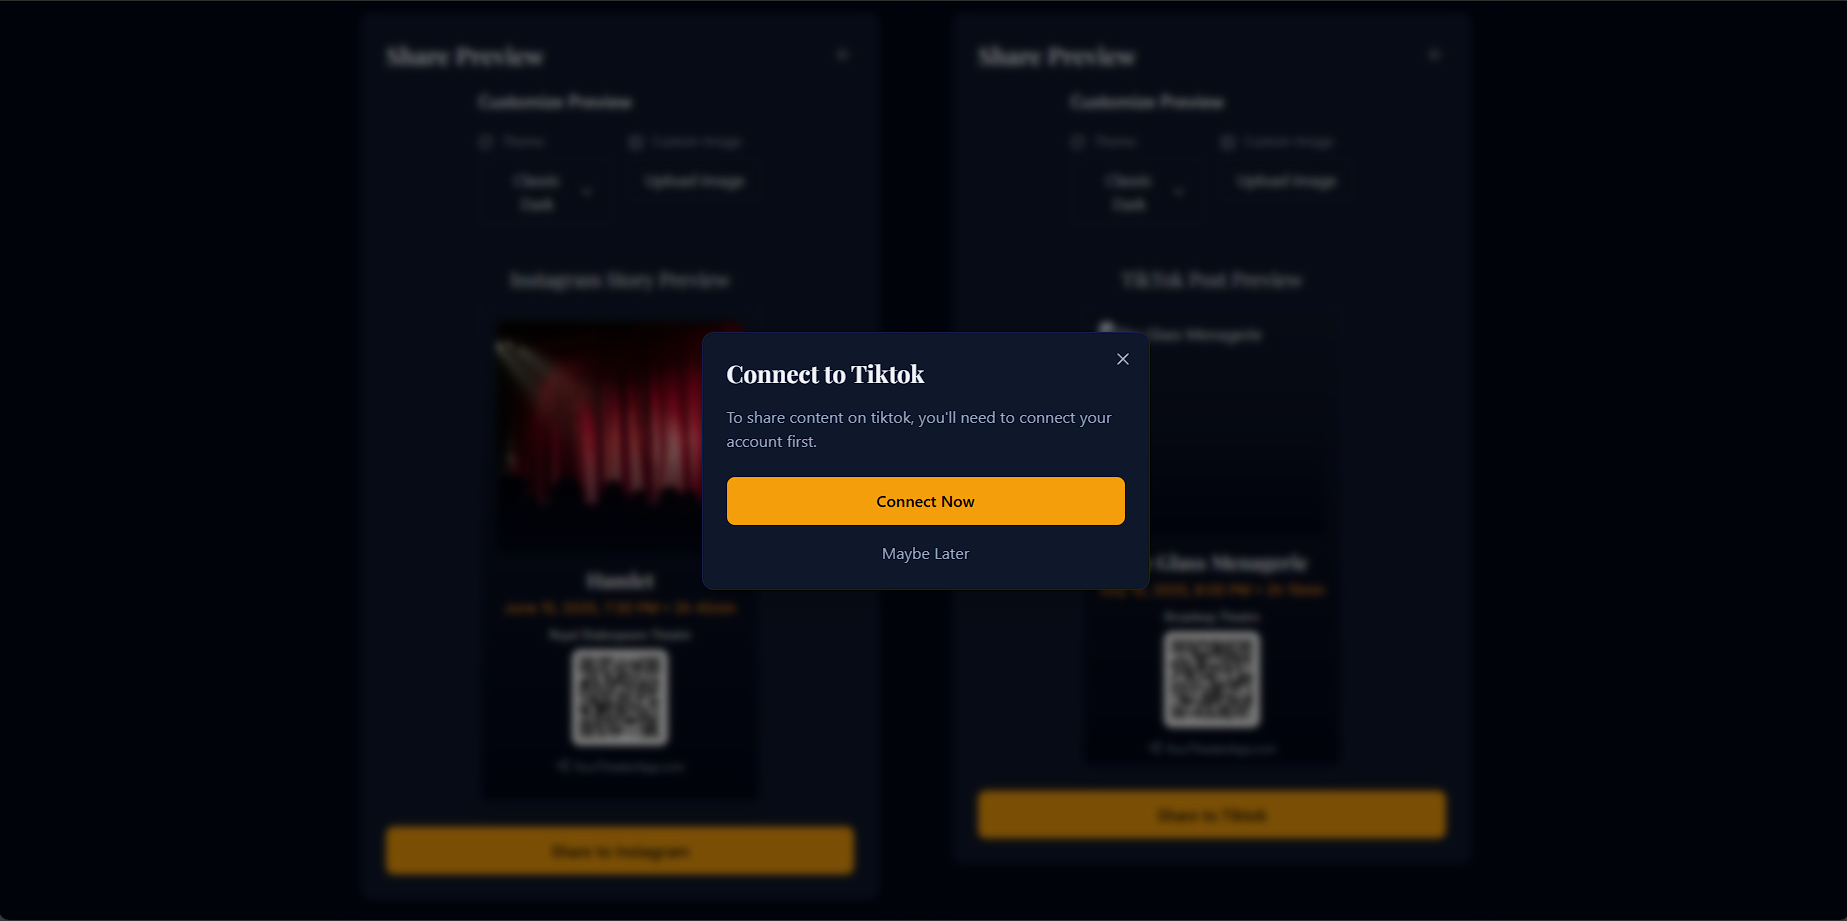
\includegraphics[width=\linewidth]{Slike/FZ5/connecttiktok.png}
        \caption{Zahtjev za povezivanje TikTok naloga}
        \label{fig:connecttitktok}
    \end{figure}

    \begin{figure}[H]
    \centering
    \begin{subfigure}[b]{0.45\textwidth}
        \centering
        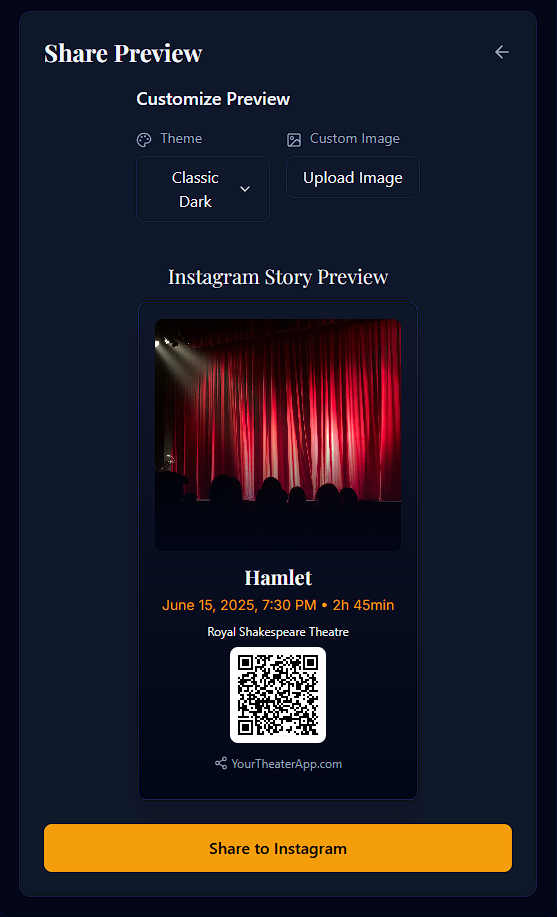
\includegraphics[width=\linewidth]{Slike/FZ5/preview.png}
        \caption{\textit{Preview} za objavu predstave putem instagrama}
        \label{fig:preview}
    \end{subfigure}
    \hfill
    \begin{subfigure}[b]{0.45\textwidth}
        \centering
        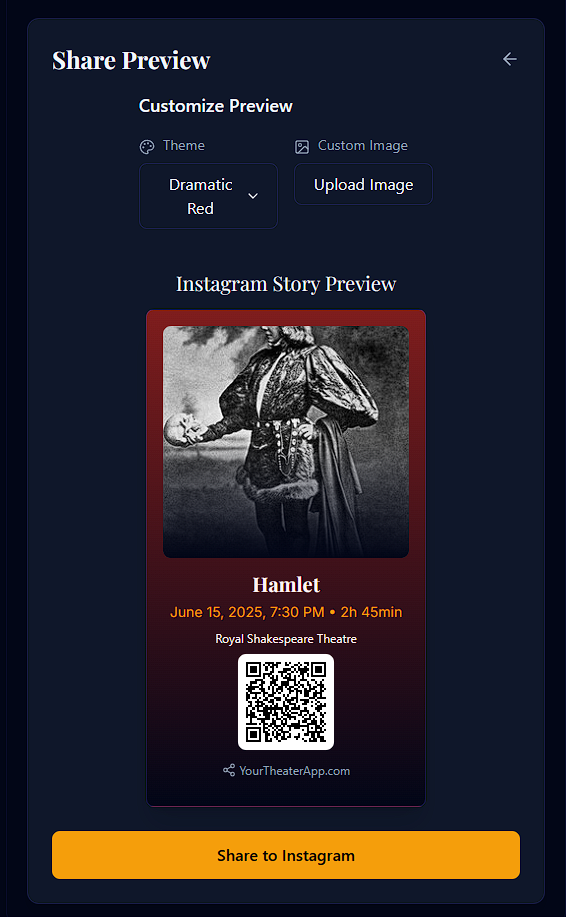
\includegraphics[width=\linewidth]{Slike/FZ5/previewchanged.png}
        \caption{Mogućnost promjene stila i/ili slike za objavu}
        \label{fig:previewchange}
    \end{subfigure}
    \caption{\textit{Preview} za dijeljenje predstave putem društvenih mreža}
\end{figure}
\end{itemize}  


\subsection{Bolt promptovi}

\begin{enumerate}[itemsep=1ex]
    \item \textbf{Prvi \textit{prompt}:}
\textit{
    Build a dark-themed UI component for a theater app that allows users to share plays on social media platforms like Instagram or TikTok.}

    \textit{Display a “Share This Play” section beneath each play.
    }
    \textit{Include buttons for Instagram and TikTok.
    }
    \textit{When clicked, generate a stylized image (poster-style) containing:
    }
    \textit{Play title, showtime, venue name, and a QR code linking back to the play’s detail page.
    }
    \textit{The image should be visually optimized for Instagram and TikTok formats.
    }
    \textit{If the user hasn’t linked their social media account, redirect them to the appropriate OAuth flow (Instagram or TikTok).
    }
    \textit{After successful OAuth, return the user to the original play page with sharing enabled.
    }
    \textit{Include feedback for the user: show a toast notification on successful share or error.
    }
    \textit{Add a preview where users can see the generated image before sharing, for example a instagram story.
    }

    \vspace{0.5cm}
    \item \textbf{Drugi \textit{prompt}:}

    \textit{Can you add the ability to edit the preview so that the user can pick the image or theme of the generated preview. Also add a  popup if the social media profile is not linked}
\end{enumerate}
\pagebreak


\sloppy  
\section{FZ6: Višekanalna korisnička podrška i komunikacija}  

\sloppy  
\subsection{Opis funkcionalnog zahtjeva}  
\begin{itemize}  
    \item \textbf{Poslovni proces}: Marketing i korisnička podrška
    \item \textbf{Vrste korisnika}: Gost/korisnik 
    \item \textbf{Scenariji korištenja}:  
    \begin{enumerate}  
        \item \textbf{Korisnik zadovoljan odgovorom \textit{chatbot}-a}

        Nakon otvaranja \textit{chat}-a, korisnik dobija odgovor na postavljeno pitanje. Problem koji je korisnik imao je riješen i korisnik napušta \textit{chat}
        
        \item \textbf{Korisnik nije zadovoljan \textit{chatbot}-om, javlja se korisničkoj podršci}

        Nakon otvaranja \textit{chat}-a, korisnik dobija odgovor na postavljeno pitanje. \textit{Chatbot} nije riješio problem, korisnik nije zadovoljan i piše poruku korisničkoj podršci putem \textit{button}-a koji iskoči.
        
        \item \textbf{Korisnik nije zadovoljan \textit{chatbot}-om i ne traži dalju pomoć}

        Nakon otvaranja \textit{chat}-a, korisnik dobija odgovor na postavljeno pitanje. \textit{Chatbot} nije riješio problem, korisnik nije zadovoljan i napušta \textit{chat} bez obraćanja korisničkoj podršci.
    \end{enumerate}  

    \item \textbf{UML dijagram aktivnosti}: Prikazan na slici \ref{fig:fz6UML}. 
    
    \vspace{0.5cm}
    
    \begin{figure}[H]
        \centering
        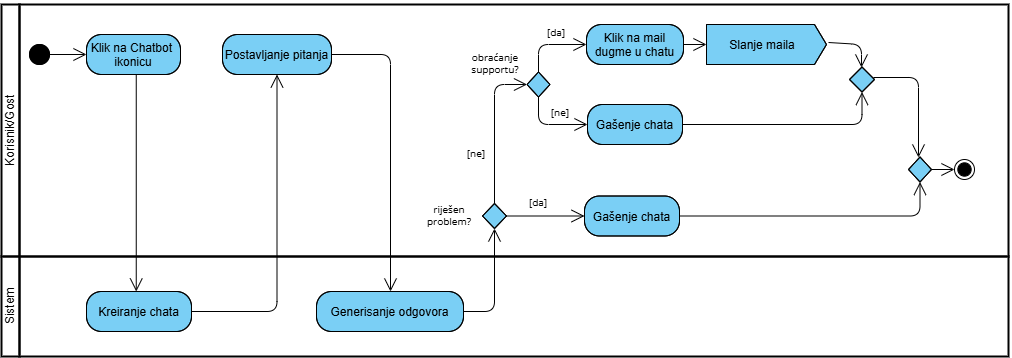
\includegraphics[width=1\linewidth]{Slike/FZ6/uml.png}
        \caption{UML dijagram za korisničku podršku i komunikaciju}
        \label{fig:fz6UML}
    \end{figure}
    
    \item \textbf{Opis scenarija}:  
    \begin{itemize}[label={--}]
        \item Korisnik otvara \textit{chatbot} i postavlja svoje pitanje,

        \item \textit{Chatbot} generiše odgovor korisniku, traži se potvrda da li je odgovor bio koristan

        \item Korisnik ima mogućnost slanja poruke korisničkoj podršci, ukoliko nije zadovoljan odgovorom, ukoliko jeste napušta \textit{chat}
    \end{itemize}
    
\end{itemize}  


\sloppy  
\subsection{Dizajn korisničkih interfejsa}  
\begin{itemize}  
    \item \textbf{Prototip interfejsa}: Na slici \ref{fig:chatbotikona} je prikazan izgled ikonice za otvaranje \textit{chatbot}-a. Slika \ref{fig:chatbeginning} prikazuje otvoreni novi \textit{chat}, a slika \ref{fig:chatresponse} izgled dijaloga sa korisnikom. Ukoliko se pritisne na \textit{thumbs down} za pitanje da li je odgovor bio koristan, iskače dugme za kontaktiranje korisničke podrške putem mejla. Na slici \ref{fig:chatsupportbutton} je prikazano dugme, a na slici \ref{fig:contactsupport} novi prozor koji se otvara u chatu za slanje mejla, nakon pritiska istog. 


\begin{figure}[H]
    \centering
    
\includegraphics[width=0.25\linewidth]{Slike/FZ6/chatbotbubble.png}
    \caption{Ikonica za otvaranje \textit{chatbota}, koja se javlja u donjem desnom uglu}
    \label{fig:chatbotikona}
\end{figure}

\begin{figure}[H]
    \centering
    \begin{subfigure}[b]{0.45\textwidth}
        \centering
        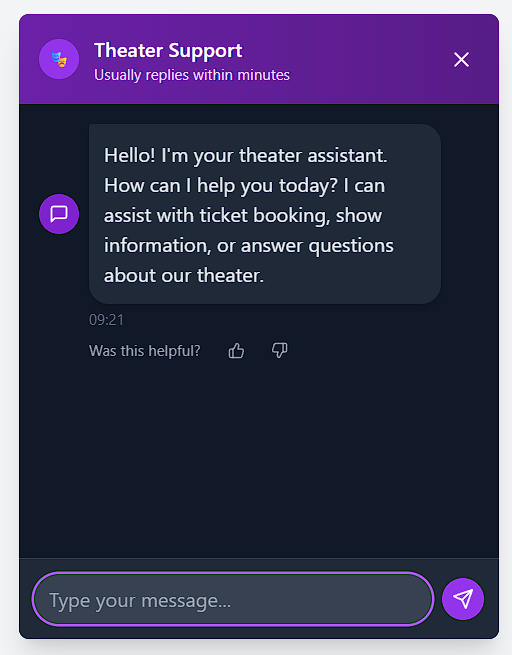
\includegraphics[width=\linewidth]{Slike/FZ6/chatbeginning.png}
        \caption{Početna poruka u \textit{chat}-u}
        \label{fig:chatbeginning}
    \end{subfigure}
    \hfill
    \begin{subfigure}[b]{0.45\textwidth}
        \centering
        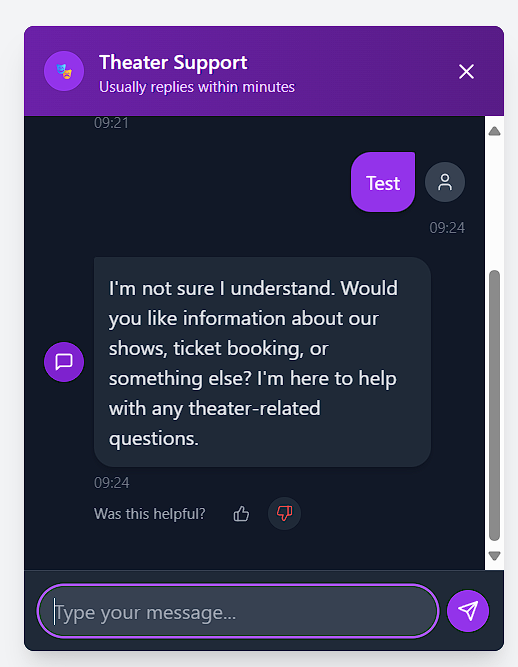
\includegraphics[width=\linewidth]{Slike/FZ6/chatresponse.png}
        \caption{Odgovor na korisničku poruku, sa \textit{hover}-om preko \textit{button}-a za loš odgovor}
        \label{fig:chatresponse}
    \end{subfigure}
    \caption{Izgled \textit{chat}-a}
\end{figure}

\begin{figure}[H]
    \centering
    \begin{subfigure}[b]{0.45\textwidth}
        \centering
        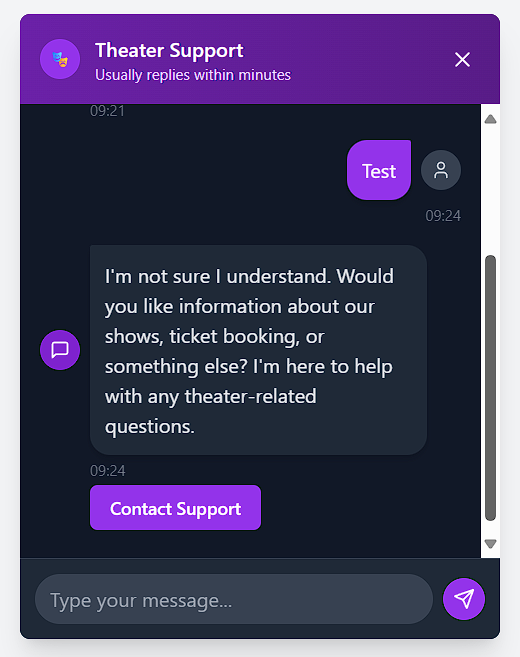
\includegraphics[width=\linewidth]{Slike/FZ6/chatsupportbutton.png}
        \caption{Prikazan \textit{button} za korisničku podršku, nakon prethodnog klika za loš odgovor}
        \label{fig:chatsupportbutton}
    \end{subfigure}
    \hfill
    \begin{subfigure}[b]{0.45\textwidth}
        \centering
        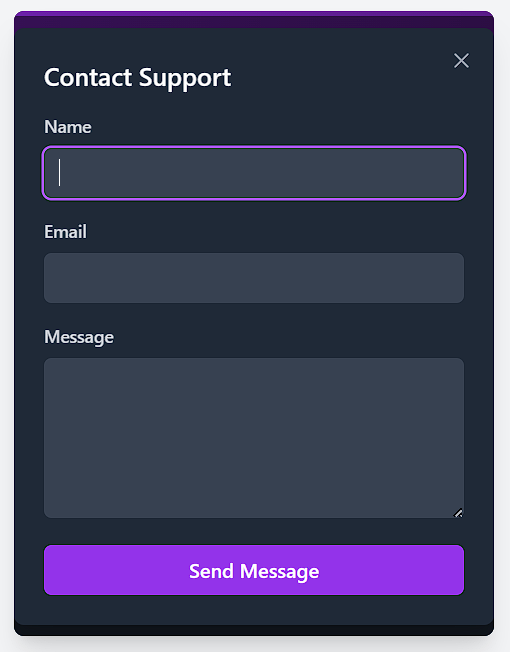
\includegraphics[width=\linewidth]{Slike/FZ6/contactsupport.png}
        \caption{Prozor za pisanje mejla nakon pritiska \textit{button}-a \textit{Contact Support}}
        \label{fig:contactsupport}
    \end{subfigure}
    \caption{Otvaranje prozora za slanje mejla korisničkoj podršci}
\end{figure}
\end{itemize}  

\subsection{Bolt promptovi}

\begin{enumerate}[itemsep=1ex]
    \item \textbf{Prvi \textit{prompt}:}

    \textit{
    Design a dark-themed customer support chatbot UI for a theater booking app. The chatbot is located in the lower-right corner of the screen and expands from a small, circular bubble when clicked. Once opened, it displays a sleek chat window with dark tones (e.g., charcoal background, subtle gradients, and soft shadows).}

    \textit{In each chat message from the bot, include:
    }
    \textit{The chatbot’s friendly response (e.g., helping with ticket booking, refund questions, or showtimes).
    }
    \textit{Below each bot response, show a "Was this helpful?" prompt with "Yes" and "No" buttons.
    }
    \textit{If the user selects "No", display a visible "Contact Support" button that opens the user's email client pre-filled to contact customer service.
    }
    \textit{The UI should be modern and minimal, with rounded message bubbles, clean typography, and subtle animations. Make sure text is highly readable in dark mode. Include example chat exchanges to illustrate the interaction flow.}

    Ovaj \textit{prompt} je proizveo grešku u kodu, koja je nakon zahtjeva za ispravku, popravljena. Nakon ispravke je generisan UI vidljiv na prethodnim slikama, s tim da se otvarao mejl klijent na računaru.

    \item \textbf{Drugi \textit{prompt}:}

    \textit{Everything looks good, but can you add a pop up window to send the email from the app itself, instead of opening the mail client.}

    Nakon ovog \textit{prompt}-a, se ispravno otvara polje za slanje mejla unutar aplikacije.    
\end{enumerate}
\pagebreak

\sloppy  
\section{FZ7: Marketing i obavještenja}  

\sloppy  
\subsection{Opis funkcionalnog zahtjeva}  
\begin{itemize}  
    \item \textbf{Poslovni proces}: Online prodaja i rezervacija karata s višestrukim načinima plaćanja 
    \item \textbf{Vrste korisnika}: Administrator, Korisnik
    \item \textbf{Scenariji korištenja}:  
        \begin{enumerate}  
            \item \textbf{Korisnik se pretplaćuje na novosti i zainteresovan je za predstavu:} 

            Administrator kreira kampanje za nove predstave, a sistem šalje notifikaciju korisniku da li se želi pretplatiti, te kada se korisnik pretplati sistem će mu slati ponude na koje on može odgovoriti da li je zainteresovan ili ne (u ovom slučaju zainteresovan) nakon čega se informacija šalje sistemu za kreiranje izvještaja koji administrator čita.
            
            \item \textbf{Korisnik se pretplaćuje na novosti i nezainteresovan je za predstavu:} 

	    Administrator kreira kampanje za nove predstave, a sistem šalje notifikaciju korisniku da li se želi pretplatiti, te kada se korisnik pretplati sistem će mu slati ponudu na koje on odgovara da nije zainteresovan te se ta informacija šalje sistemu za kreiranje izvještaja koji administrator čita.            

            \item \textbf{Korisnik obija da se pretplati na novosti:} 

            Administrator kreira kampanje za nove predstave, a sistem šalje notifikaciju korisniku da li se želi pretplatiti na šta on odgovara da ne želi te se ta informacija proslijeđuje sistemu za kreiranje izvještaja koji čita administrator.  
        \end{enumerate}
    \item \textbf{UML dijagram aktivnosti}: Prikazan na slici \ref{fig:fz7}  
\end{itemize}  
\begin{figure}[H]
        \centering
        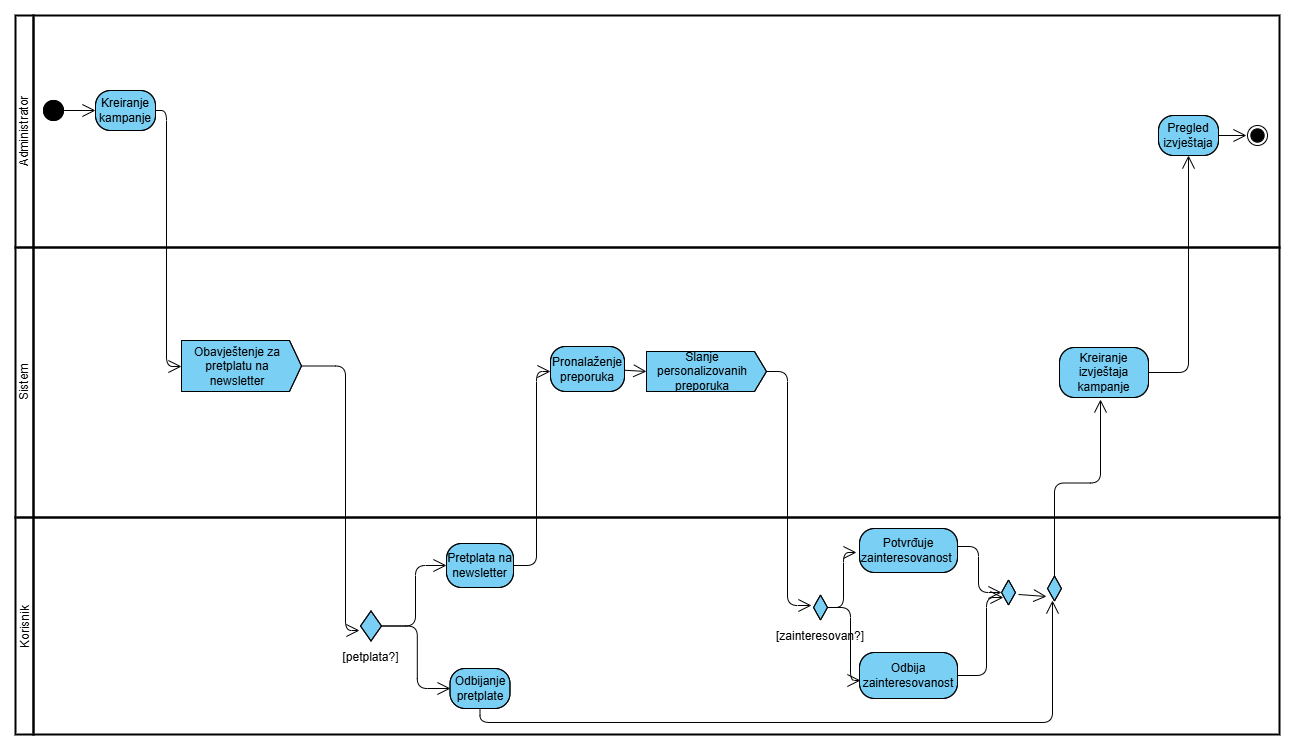
\includegraphics[width=1\linewidth]{Slike/FZ7.png}
        \caption{UML dijagram za marketing i obavještenja}
        \label{fig:fz7}
    \end{figure}
\sloppy  
\subsection{Dizajn korisničkih interfejsa}  
\begin{itemize}  
    \item \textbf{Prototip interfejsa}: 
    \begin{itemize}
        \item Administratorski ekran za kreiranje kampanja i čitanje izvještaja kampanja. Slike \ref{fig:fz7.1} i \ref{fig:fz7.2}.
        \item Korisnički ekran sa notifikacijom o pretplati na novosti. Slika \ref{fig:fz7.3}.
        \item Korisnički ekran sa notifikacijom o novoj predstavi gdje dugme zainteresovan vodi na kupovinu karte. Slika \ref{fig:fz7.4}.
    \end{itemize}
    \item \textbf{Opis scenarija}:  
        \begin{itemize}  
            \item Administrator kraira kampanju i šalje obavijesti.  
            \item Korisnik se pretplaćuje na novosti te prima notifikacije o novim predstavama.  
        \end{itemize}  
\end{itemize}  
\begin{figure}[H]
        \centering
        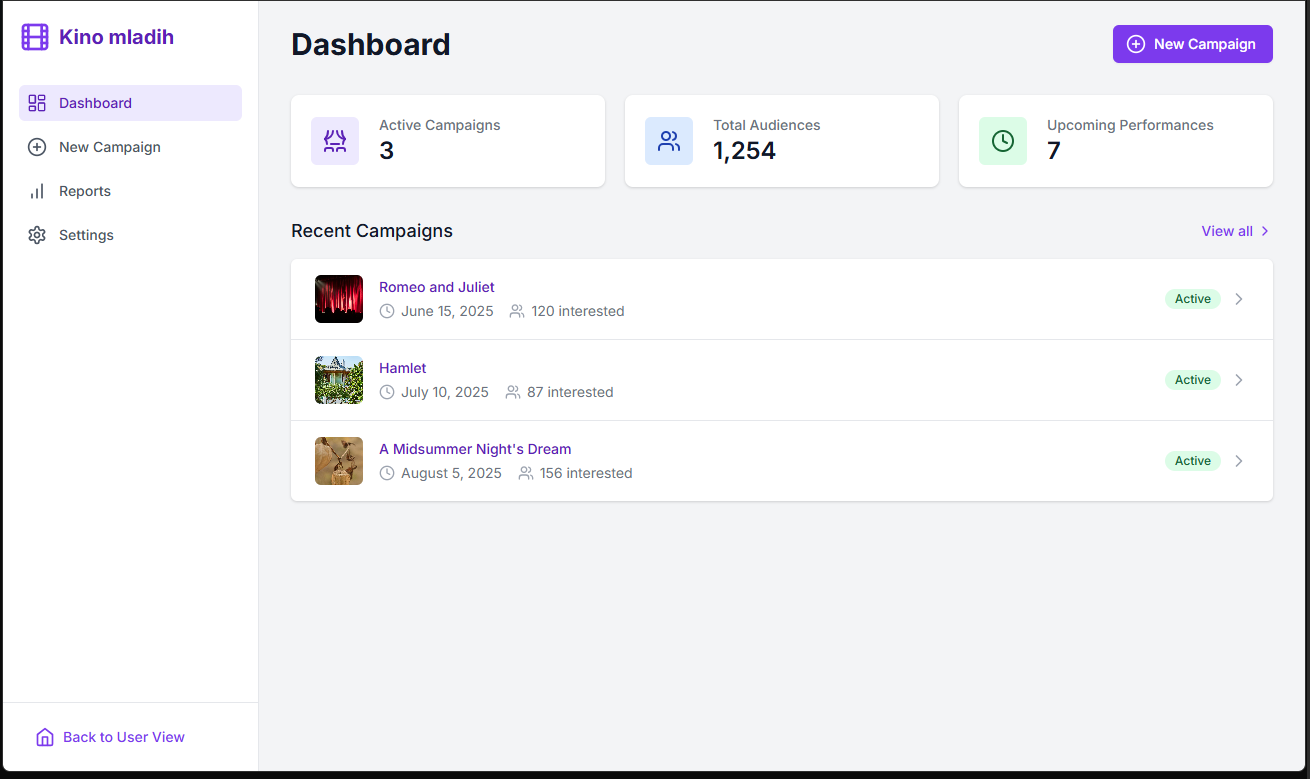
\includegraphics[width=1\linewidth]{Slike/FZ7.1.PNG}
        \caption{Administratorski prikaz aktivnih kampanja i interesovanja}
        \label{fig:fz7.1}
    \end{figure} 
    \begin{figure}[H]
        \centering
        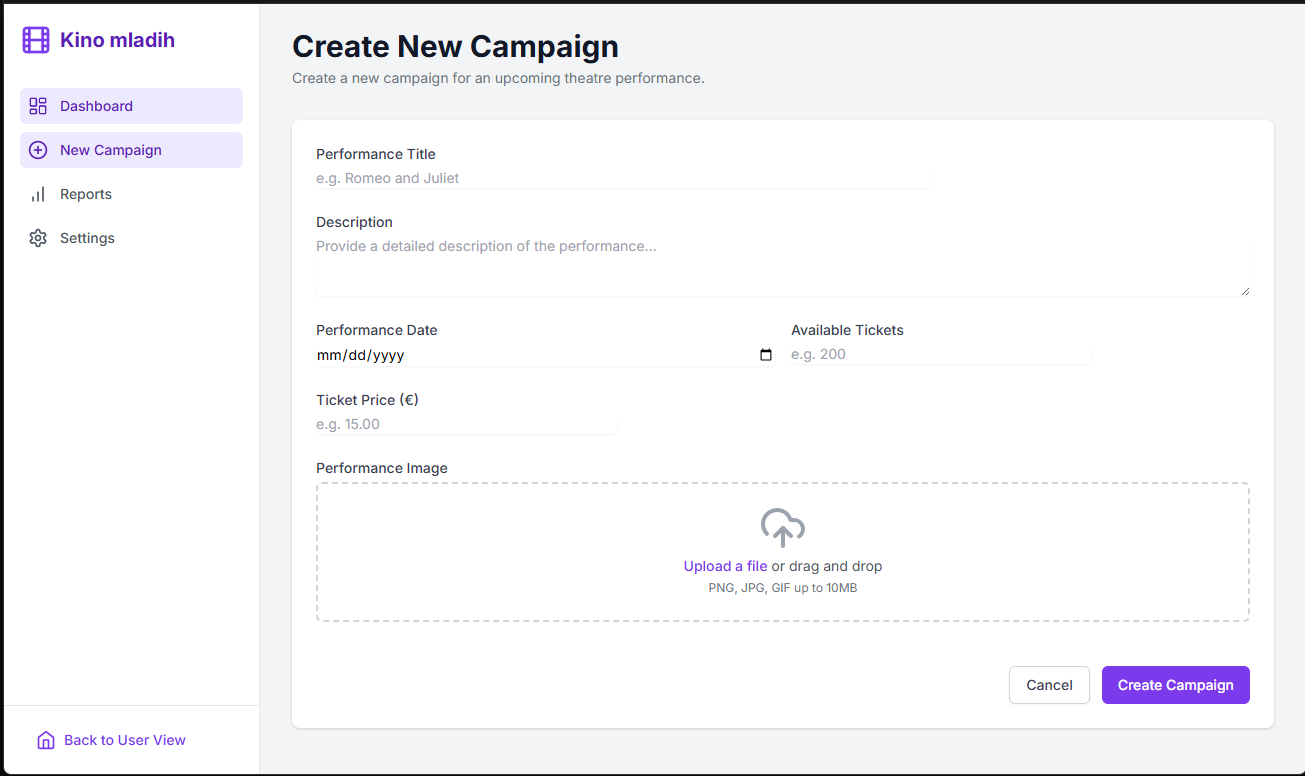
\includegraphics[width=1\linewidth]{Slike/FZ7.2.PNG}
        \caption{Kreiranje nove kampanje}
        \label{fig:fz7.2}
    \end{figure}
    \begin{figure}[H]
        \centering
        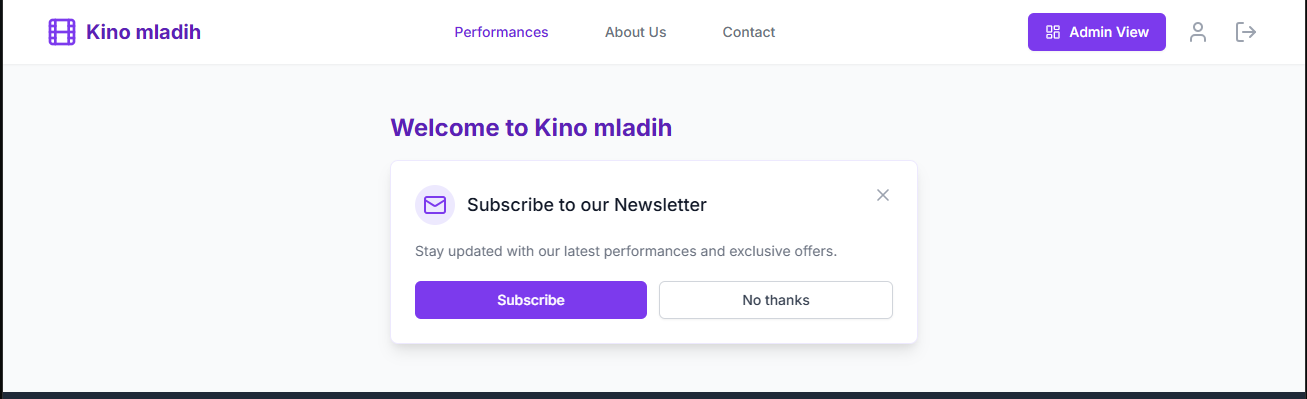
\includegraphics[width=1\linewidth]{Slike/FZ7.3.PNG}
        \caption{Notifikacija za pretplatu na novosti}
        \label{fig:fz7.3}
    \end{figure}
    \begin{figure}[H]
        \centering
        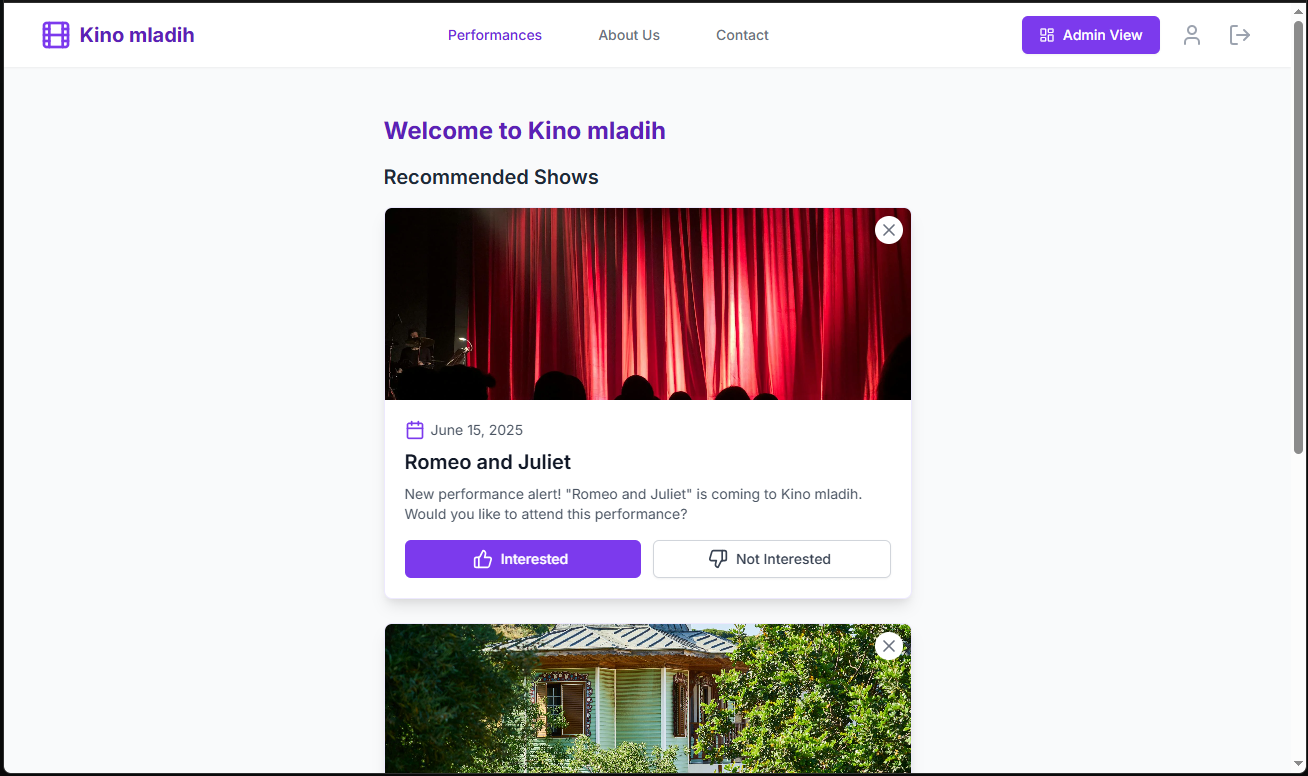
\includegraphics[width=1\linewidth]{Slike/FZ7.4.PNG}
        \caption{Notifikacija o preporučenim predstavama}
        \label{fig:fz7.4}
    \end{figure}
\sloppy  

\subsection{Bolt \textit{promptovi}}

\begin{enumerate}[itemsep=1ex]
    \item \textbf{Prvi \textit{prompt}:}

    \textit{
    Design a clean and modern web interface for a platform called "Kino mladih" (Youth Cinema) with a white and purple color scheme. Include the following screens:Admin dashboard,Section to create a new campaign for upcoming theatre performances. Section to view campaign reports, including a list of interested and uninterested users.,User screen - Subscription Notification. Modal or banner with a question: "Do you want to subscribe to our newsletter?" Buttons for [Subscribe] and [No thanks]. User screen - New Performance Alert Notification about a new theatre performance. Button labeled "Interested" that leads to the ticket purchase page. Option to mark as "Not Interested". The overall design should be minimalistic and elegant, using white backgrounds with vibrant purple accents, soft shadows, modern sans-serif fonts, and intuitive UI elements.}
    \item \textbf{Drugi \textit{prompt}:}

    \textit{Remove "Enter your email" and add button to switch to admin view with reports. Also for use- show recommended shows only after subscribe is clicked.}    
\end{enumerate}
\section{FZ8: Personalizovane notifikacije o novim predstavama i ponudama} 
\sloppy  
\subsection{Opis funkcionalnog zahtjeva}  
\begin{itemize}  
    \item \textbf{Poslovni proces}: Kreiranje i uređivanje korisničkih profila  
    \item \textbf{Vrste korisnika}: Registrovani korisnik
    \item \textbf{Scenariji korištenja}:  
        \begin{enumerate}  
            \item \textbf{Uređivanje personalizovanih notifikacija:} 

		Uređivanje personalizovanih notifikacija za unaprijeđenje algoritma preporuka, kao i promjena načina slanja notifikacija. Mogućnost odabira 5 najboljih predstava za korisnika u narednoj sedmici. 
            \item \textbf{Potvrđivanje zadovoljstva notifikacijama:} 

	Pozitivna povratna informacija tj. korisnik je zadovoljan notifikacijama.    
        \end{enumerate}  
    \item \textbf{UML dijagram aktivnosti}: Prikazan na slici \ref{fig:fz8}  
\end{itemize}  
\begin{figure}[H]
        \centering
        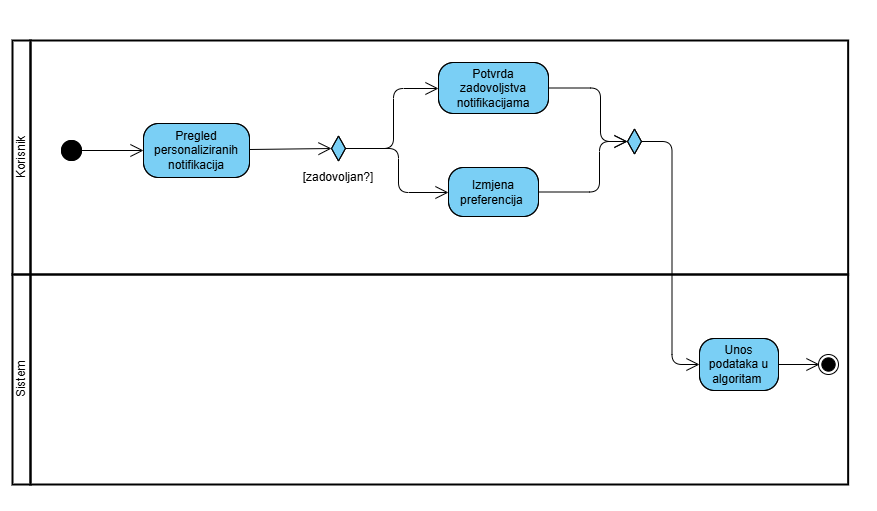
\includegraphics[width=1\linewidth]{Slike/FZ8.png}
        \caption{UML dijagram za prilagođavanje notifikacija}
        \label{fig:fz8}
    \end{figure}
\sloppy  
\subsection{Dizajn korisničkih interfejsa}  
\begin{itemize}  
    \item \textbf{Prototip interfejsa}: Postavke profila s opcijama za personalizovane notifikacije. Slike \ref{fig:fz8.1} i \ref{fig:fz8.2}. 
    \item \textbf{Opis scenarija}:  
        \begin{itemize}  
            \item Korisnik odabire tipove notifikacija koje želi da prima i načine slanja notifikacija. Mogućnost izlistavanja najboljih 5 predstava u narednoj sedmici za korisnika. 
        \end{itemize}  
\end{itemize}  
\begin{figure}[H]
        \centering
        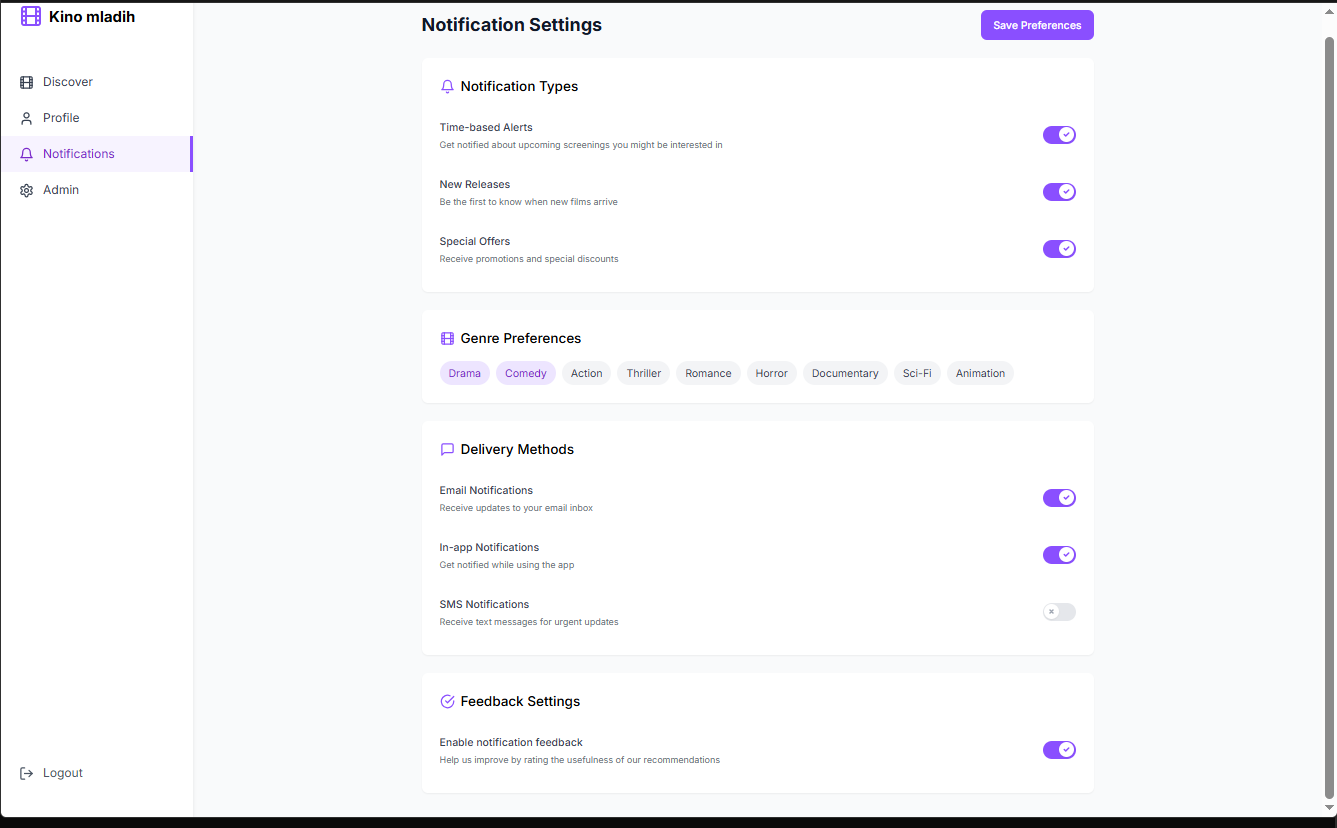
\includegraphics[width=1\linewidth]{Slike/FZ8.1.PNG}
        \caption{Uređivanje personalizovanih notifikacija}
        \label{fig:fz8.1}
    \end{figure}
    \begin{figure}[H]
        \centering
        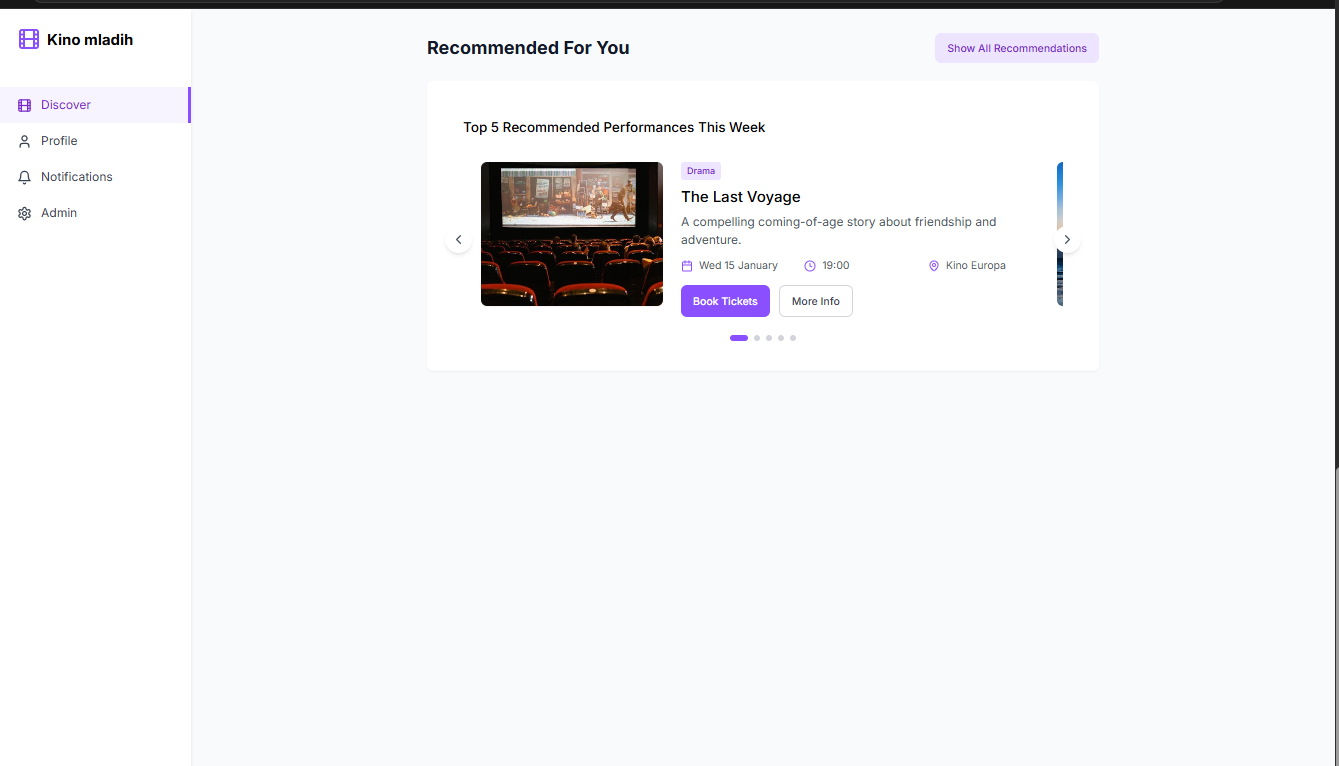
\includegraphics[width=1\linewidth]{Slike/FZ8.2.PNG}
        \caption{Najboljih 5 predstava za korisnika}
        \label{fig:fz8.2}
    \end{figure}
\sloppy  
\pagebreak
\subsection{Bolt \textit{promptovi}}

\begin{enumerate}[itemsep=1ex]
    \item \textbf{Prvi \textit{prompt}:}

    \textit{
    Design a sleek and user-friendly web interface for the platform "Kino mladih" (Youth Cinema), using a white and purple color scheme. Focus on profile settings and notification personalization. Include the following screens: User Profile Settings Screen. Section to customize types of notifications (e.g. genre preferences, time-based alerts). Options for notification delivery methods (email, in-app, SMS). Button to "Show Top 5 Recommended Performances This Week" with a card-style preview layout. Toggle for giving feedback on notification usefulness (e.g. "These recommendations are helpful"). Admin Promo Panel (Optional Screen). A simple interface for the administrator to send seasonal promotional campaigns to all subscribed users. Option to segment the audience based on notification settings or interests. Keep the design minimal, modern, and intuitive with white backgrounds, purple accent buttons, soft shadows, and rounded UI elements.}
\end{enumerate}
\sloppy  
\section{FZ9: Moderacija foruma}  

\sloppy  
\subsection{Opis funkcionalnog zahtjeva}  
\begin{itemize}  
    \item \textbf{Poslovni proces}: Forum za predstave.  
    \item \textbf{Vrste korisnika}: Administrator.  
    \item \textbf{Scenariji korištenja}:  
        \begin{enumerate}  
            \item \textbf{Brisanje komentara:}
            Administrator pregleda sve komentare na forumu. Nakon uočavanja neprimjerenih komentara on vrši brisanje ili upozoravanje tih komentara koji krše pravila foruma.   
            \item \textbf{Ažuriranje forum pravila:} 
            Administrator pregleda sva trenutna pravila. Postavljanje nova forum pravila po želji.  
        \end{enumerate}  
    \item \textbf{UML dijagram aktivnosti}: Prikazan na slici \ref{fig:fz9_uml}  
    \begin{figure}[H]
        \centering
        \includegraphics[width=1\linewidth]{Slike/FZ9/FZ9_UML.png}
        \caption{UML dijagram aktivnosti "Moderacija foruma"}
        \label{fig:fz9_uml}
    \end{figure}
\end{itemize}  
\sloppy  
\subsection{Dizajn korisničkih interfejsa}  
\begin{itemize}  
    \item \textbf{Prototip interfejsa}: Moderatorski panel s opcijama "Obriši", "Upozori korisnika" (slike \ref{fig:fz9_1} i \ref{fig:fz9_2}).  
    \item \textbf{Opis scenarija}:  
    \begin{itemize}  
            \item Administrator pregleda nove komentare. On uklanjanja one koji krše pravila foruma koje je on postavio. 
            \item Administrator pregleda filter za automatsko blokiranje određenih riječi. On ažurira taj filter, dodavajući ili brišući riječi koje hoće da blokira.  
        \end{itemize}  
    \begin{figure}[H]
        \centering
        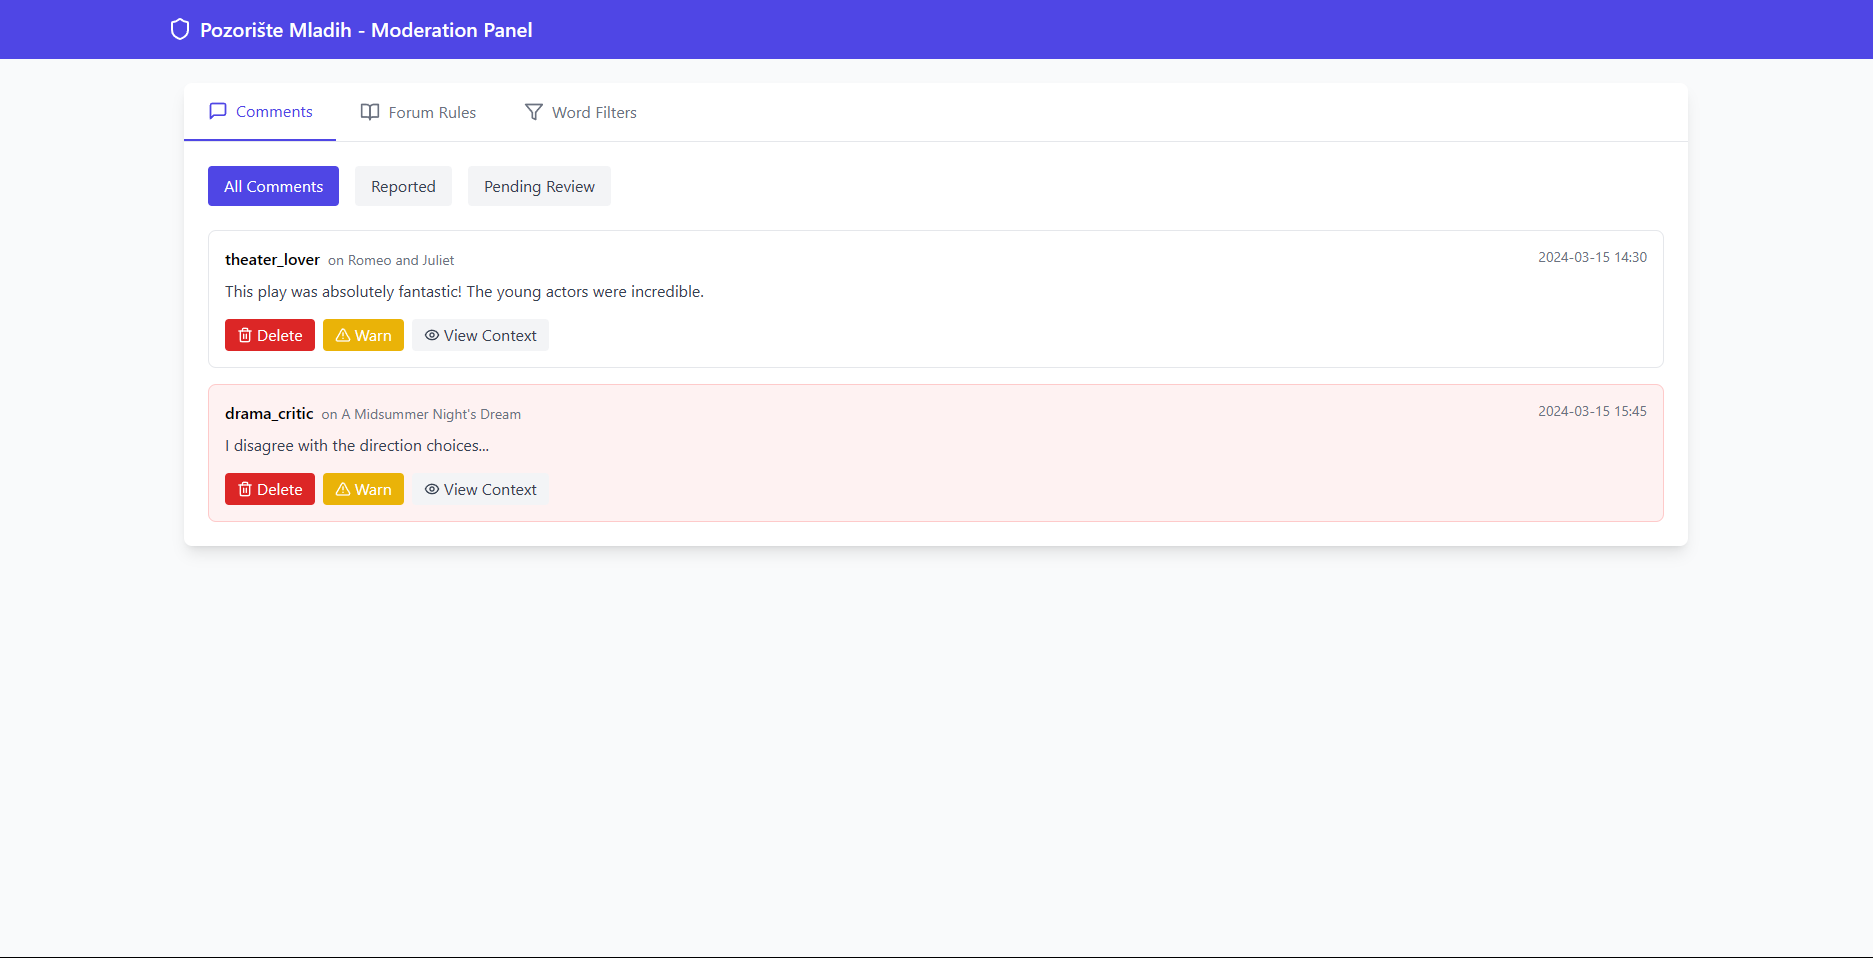
\includegraphics[width=1\linewidth]{Slike/FZ9/fz9_1.png}
        \caption{Moderator pregleda nove komentare i uklanja one koji krše pravila}
        \label{fig:fz9_1}
    \end{figure}
    \begin{figure}[H]
        \centering
        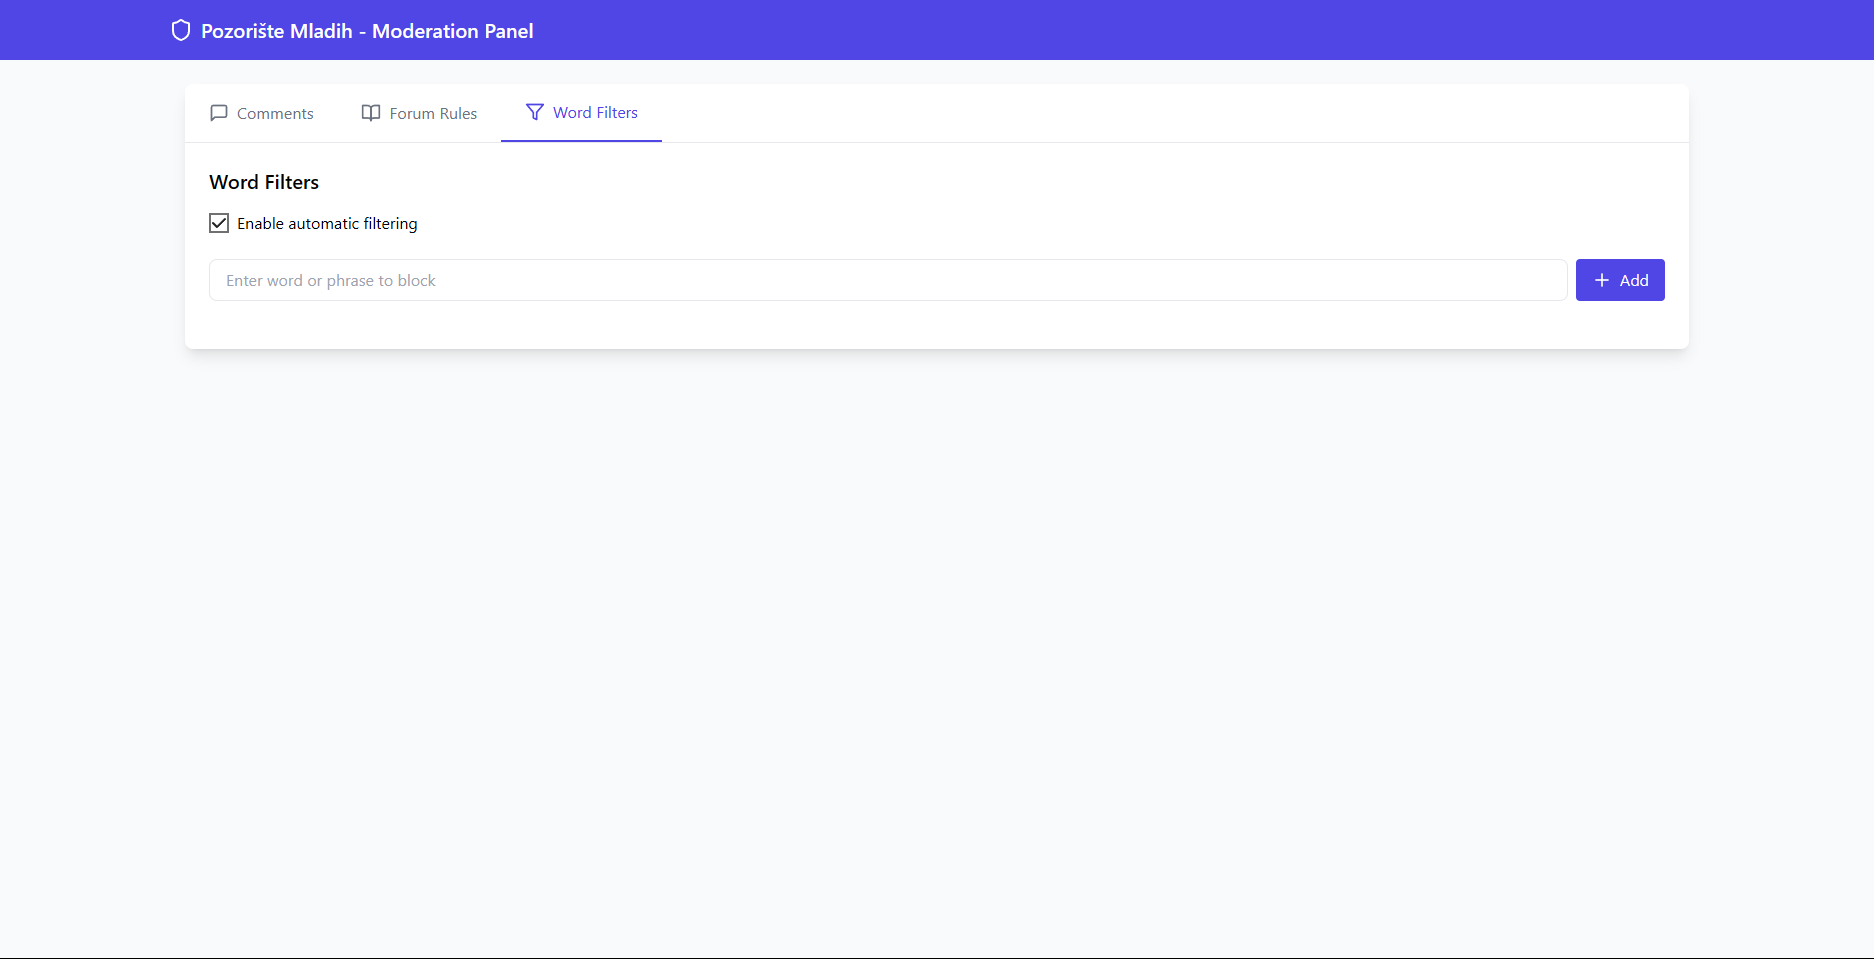
\includegraphics[width=1\linewidth]{Slike/FZ9/fz9_2.png}
        \caption{Administrator postavlja filtere za automatsko blokiranje određenih riječi.}
        \label{fig:fz9_2}
    \end{figure}
\end{itemize}  

\sloppy  
\subsection{Bolt \textit{promptovi}}

\begin{enumerate}[itemsep=1ex]
    \item \textbf{Prvi \textit{prompt}:}

    \textit{
    Design a User Interface for Forum Moderation for a "Pozorište Mladih" (Youth Theatre) application. The interface should be clean, intuitive, and primarily for users with Administrator or Moderator roles.}

    \textit{
    The UI should include the following components and functionalities:}
    
    \textit{Moderator Dashboard/Panel:}
    
    \textit{A central view for managing forum content.}
    \textit{Comment Listing: Display a list of forum comments, potentially filterable by "all," "reported," "pending review" (if applicable). Each comment entry should show:}
    \textit{The content of the comment.}
    \textit{The username of the poster.}
    \textit{Date and time of posting.}
    \textit{The specific play/thread the comment belongs to.}
    \textit{Moderation Actions per Comment: For each comment, provide clear action buttons such as:}
    \textit{[Delete Comment] - To remove the comment.}
    \textit{[Warn User] - To send a predefined or custom warning to the user who posted the comment. This might open a small modal to confirm or customize the warning.}
    \textit{[View Context] - To see the comment within its original thread.}
    \textit{Bulk Actions (Optional): Ability to select multiple comments and apply an action like "Delete Selected."}
    
    \textit{Forum Rules Management (Administrator Access):}
    
    \textit{A dedicated section where an Administrator can:}
    \textit{View the current forum rules.}
    \textit{Edit the forum rules using a rich text editor or a simple text area.}
    \textit{A [Save Rules] button to update the publicly visible forum rules.}
    
    \textit{Automated Filtering/Blocked Words Management (Administrator Access):}
    
    \textit{A section where an Administrator can manage a list of words or phrases that should be   automatically flagged or blocked from posts.}
    \textit{An input field to [Add New Word/Phrase] to the filter list.}
    \textit{A display of the current list of blocked words/phrases, with an option to [Remove] individual entries.}
    \textit{A toggle to enable/disable the automatic filter.}
    
    \textit{Key Scenarios to Visualize:}
    
    \textit{Scenario 1 (Moderator - Deleting a comment): A Moderator sees a list of comments, identifies an inappropriate one, and clicks the "Delete Comment" button next to it. A confirmation prompt might appear.}
    \textit{Scenario 2 (Administrator - Setting Forum Rules): An Administrator navigates to the "Forum Rules Management" section, types in or edits the rules in a text area, and clicks "Save Rules."}
    \textit{Scenario 3 (Administrator - Adding a blocked word): An Administrator goes to the "Automated Filtering" section, types a new word into the "Add New Word/Phrase" field, and adds it to the list.}
    \textit{The overall design should be professional, easy to navigate, and clearly distinguish between different management areas. Consider using a clean layout with clear visual cues for actionable items.}

\end{enumerate}
\sloppy  

\sloppy  
\section{FZ10: Detaljna analitika i izvještavanje za administratore}  

\sloppy  
\subsection{Opis funkcionalnog zahtjeva}  
\begin{itemize}  
    \item \textbf{Poslovni procesi}: Upravljanje reportoarom i prodajom karata, Forum za predstave.  
    \item \textbf{Vrste korisnika}: Administrator.  
    \item \textbf{Scenariji korištenja}:  
        \begin{enumerate}  
            \item \textbf{Generisanje izvještaja o mjesečnoj prodaji:} 
            Administrator klika "Export PDF" dugme. Sistem generiše izvještaj o mjesečnoj prodaji.  
            \item \textbf{Pregled angažmana publike na forumu:} Administrator vrši pregled angažmana publike na forumu. Tu vidi sve podatke o korisničkim radnjama na forumu.  
        \end{enumerate}  
    \item \textbf{UML dijagram aktivnosti}: Prikazan na slici \ref{fig:fz10_uml}  
    \begin{figure}[H]
        \centering
        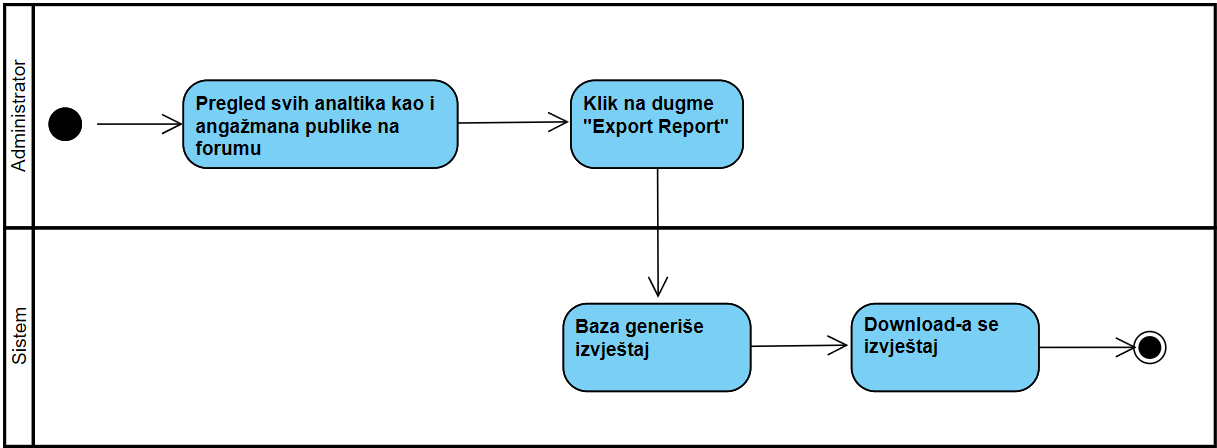
\includegraphics[width=1\linewidth]{Slike/FZ10/fz10_uml.png}
        \caption{UML dijagram aktivnosti "Detaljna analitika i izvještavanje za administratore"}
        \label{fig:fz10_uml}
    \end{figure}
\end{itemize}  

\sloppy  
\subsection{Dizajn korisničkih interfejsa}  
\begin{itemize}  
    \item \textbf{Prototip interfejsa}: Dashboard s graficima prodaje i filterima po vremenu/tipu predstave (slike \ref{fig:fz10_1}, \ref{fig:fz10_2}, \ref{fig:fz10_3} i \ref{fig:fz10_4}).  
    \item \textbf{Opis scenarija}:  
        \begin{itemize}  
            \item Administrator vrši pregled analitike finansijskog odjela. Potom eksportuje PDF izvješraj za finansijski odjel.   
            \item Administrator vrši pregled najpopularnijih predstava. Predstave su poredane prema ocjenama korisnika, od najbolje ocjenjenih do najgore ocjenjenih.  
        \end{itemize} 
    \begin{figure}[H]
        \centering
        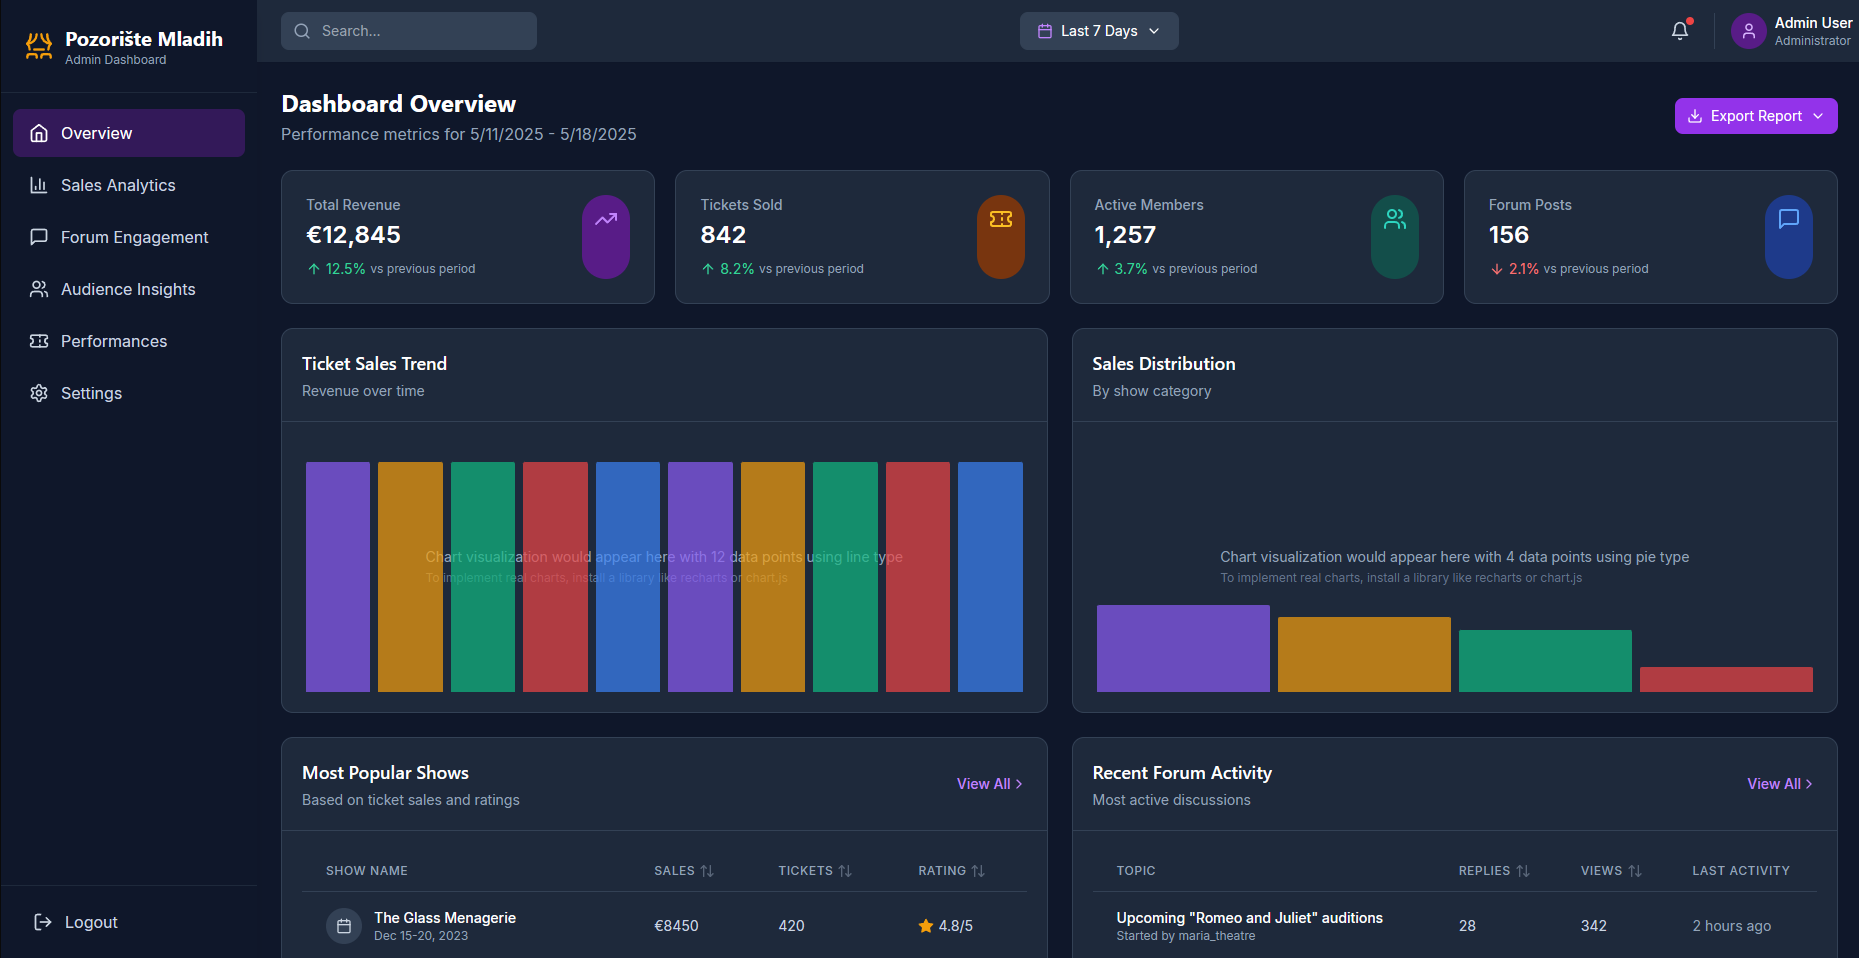
\includegraphics[width=1\linewidth]{Slike/FZ10/fz10_1.png}
        \caption{Overview svih podataka}
        \label{fig:fz10_1}
    \end{figure}
    \begin{figure}[H]
        \centering
        \includegraphics[width=1\linewidth]{Slike/FZ10/fz10_2.png}
        \caption{Analitika prodaje}
        \label{fig:fz10_2}
    \end{figure}
    \begin{figure}[H]
        \centering
        \includegraphics[width=1\linewidth]{Slike/FZ10/fz10_3.png}
        \caption{Analitika foruma}
        \label{fig:fz10_3}
    \end{figure}
    \begin{figure}[H]
        \centering
        \includegraphics[width=1\linewidth]{Slike/FZ10/fz10_4.png}
        \caption{Analitika publike}
        \label{fig:fz10_4}
    \end{figure}
\end{itemize}  

\sloppy  
\subsection{Bolt \textit{promptovi}}

\begin{enumerate}[itemsep=1ex]
    \item \textbf{Prvi \textit{prompt}:}

    \textit{Design a comprehensive Administrator Dashboard for a "Pozorište Mladih" (Youth Theatre) application, focusing on detailed analytics and reporting. The UI should be clean, modern, and intuitive, enabling administrators to easily understand performance metrics.}

    \textit{The dashboard should consist of several key sections:}

    \textit{Main Dashboard Overview:}

    \textit{Prominently display Key Performance Indicators (KPIs) such as:}
    \textit{Total ticket sales (revenue and number of tickets) for a selected period.}
    \textit{Most popular upcoming/current shows.}
    \textit{Recent forum activity highlights (e.g., new posts, most discussed topics).}
    \textit{Allow selection of a global date range (e.g., Last 7 Days, Last 30 Days, Custom Range) that applies to many dashboard widgets.}
    
    \textit{Sales Analytics Section:}

    \textit{Detailed Sales Reports:}
    \textit{Display total revenue, number of tickets sold, and average ticket price.}
    \textit{Breakdown of sales by individual show.}
    \textit{Sales trends over time (e.g., daily, weekly, monthly sales shown in a line chart).}
    \textit{Filtering Options:}
    \textit{Filter sales data by date range.}
    \textit{Filter by specific show or show type (if applicable).}
    \textit{Data Visualization:}
    \textit{Use clear charts (e.g., bar charts for sales per show, line charts for trends, pie charts for revenue contribution by show).}
    \textit{Include data tables for detailed numerical views.}
    \textit{Export Functionality:}
    \textit{A clear [Export Report] button, allowing administrators to download sales reports (e.g., in PDF format for financial departments, CSV for further analysis). The export should respect currently applied filters.}
    
    \textit{Forum Engagement Analytics Section:}

    \textit{Activity Metrics:}
    \textit{Total number of forum posts and comments over a selected period.}
    \textit{Number of active users on the forum.}
    \textit{List of most active/discussed threads or shows.}
    \textit{User Feedback \& Ratings:}
    \textit{Aggregate user ratings for shows (e.g., average rating per show).}
    \textit{Display a list of "Most Popular Shows by User Rating."}
    \textit{Data Visualization:}
    \textit{Graphs showing trends in forum activity (e.g., posts per day).}
    \textit{Tables listing shows with their average ratings and number of reviews.}
    
    \textit{Audience Insights (Optional, but good to consider):}
    
    \textit{Demographics of registered users (if this data is collected and permissible).}
    \textit{Preferences based on past ticket purchases or forum activity.}
    
    \textit{Key Scenarios to Visualize:}

    \textit{Scenario 1 (Generating Monthly Sales Report): An administrator navigates to the Sales Analytics section, selects "Last Month" as the date range, and clicks [Export Report] to get a PDF.}
    \textit{Scenario 2 (Reviewing Forum Engagement): An administrator goes to the Forum Engagement section to see which shows are currently generating the most discussion and what their average user ratings are.}
    \textit{Scenario 3 (Identifying Popular Shows): An administrator looks at the dashboard overview or a dedicated "Popular Shows" section (which might combine sales data and user ratings) to understand which performances are most successful.}
    \textit{Overall Design Considerations:}

    \textit{The design should be professional and data-driven.}
    \textit{Prioritize readability of charts and data tables.}
    \textit{Ensure intuitive navigation between different analytics sections.}
    \textit{Use a consistent visual style, potentially aligning with the theatre's branding.}

\end{enumerate}
\sloppy




\textbf{TEMPLATE AKO NEKO PREPRAVLJA}
\section{FZ1: Naziv funkcionalnog zahtjeva}

Za svaki funkcionalni zahtjev kreirati posebno podpoglavlje (ukupno 10 podpoglavlja).

\sloppy
\subsection{Opis funkcionalnog zahtjeva}

Ukratko opisati funkcionalni zahtjev i kojem poslovnom procesu pripada, kao i koje vrste korisnika u njemu učestvuju. Navesti koliko je ukupno scenarija korištenja (alternativnih tokova). Naposlijetku vizualizirati funkcionalni zahtjev putem UML dijagrama aktivnosti.

\sloppy
\subsection{Dizajn korisničkih interfejsa}

Prikazati i opisati sve prototipe korisničkih interfejsa koji služe za ostvarivanje datog funkcionalnog zahtjeva. Za prikaz i opis koristiti sve moguće scenarije korištenja.